\documentclass[11pt,a4paper]{report}
\usepackage[T1]{fontenc}
\usepackage{mathpazo}
\usepackage[scaled=0.92]{helvet}
\usepackage[varqu,varl,scaled=0.96]{zi4}   % Inconsolata: a narrower, clearer monospace than Courier
\usepackage[protrusion=true,expansion=true]{microtype}
\usepackage[a4paper,margin=2.5cm,headheight=14pt]{geometry}
\usepackage{amsmath,amssymb}
\usepackage{booktabs,longtable,array,tabularx,multirow}
\usepackage{graphicx}
\usepackage[table]{xcolor}
\definecolor{brand}{HTML}{1F4E79}
\definecolor{brandlight}{HTML}{E3ECF6}
\definecolor{rowgray}{gray}{0.965}
\usepackage{tikz}
\usetikzlibrary{arrows.meta,positioning,shapes.geometric,calc,fit,backgrounds,decorations.pathmorphing,patterns}
\usepackage{algorithm}
\usepackage{algpseudocode}
\usepackage{listings}
\usepackage{caption}
\captionsetup{font=small,labelfont={bf,color=brand},skip=6pt}
\captionsetup[table]{position=top}
\usepackage[most]{tcolorbox}
\usepackage{needspace}
\usepackage{float}
\usepackage{etoolbox}
\usepackage{titlesec}
\titleformat{\chapter}[display]{\normalfont\color{brand}}{\sffamily\large\bfseries\MakeUppercase{\chaptertitlename}\ \thechapter}{4pt}{\raggedright\sffamily\huge\bfseries}[\vspace{3pt}{\titlerule[0.8pt]}]
\titlespacing*{\chapter}{0pt}{0pt}{18pt}
\titleformat{\section}{\needspace{8\baselineskip}\raggedright\normalfont\sffamily\Large\bfseries\color{brand}}{\thesection}{0.7em}{}
\titleformat{\subsection}{\needspace{6\baselineskip}\raggedright\normalfont\sffamily\large\bfseries\color{brand!80!black}}{\thesubsection}{0.7em}{}
\titleformat{\subsubsection}{\needspace{6\baselineskip}\normalfont\sffamily\normalsize\bfseries}{\thesubsubsection}{0.7em}{}
\titlespacing*{\section}{0pt}{16pt plus 4pt minus 2pt}{6pt}
\titlespacing*{\subsection}{0pt}{12pt plus 3pt minus 2pt}{4pt}
\usepackage{fancyhdr}
\pagestyle{fancy}
\fancyhf{}
\fancyhead[L]{\small\sffamily\color{gray}\leftmark}
\fancyhead[R]{\small\sffamily\color{gray}Raven--MODFLOW~6 groundwater coupling}
\fancyfoot[C]{\small\sffamily\thepage}
\renewcommand{\headrulewidth}{0.4pt}
\renewcommand{\chaptermark}[1]{\markboth{\thechapter\quad #1}{}}
\fancypagestyle{plain}{\fancyhf{}\fancyfoot[C]{\small\sffamily\thepage}\renewcommand{\headrulewidth}{0pt}}
\usepackage[colorlinks=true,linkcolor=brand,citecolor=brand,urlcolor=brand]{hyperref}
\emergencystretch=6em
\setcounter{secnumdepth}{3}
\setcounter{tocdepth}{1}
\makeatletter\patchcmd{\l@chapter}{\addvspace{1.0em \@plus\p@}}{\addvspace{0.45em \@plus\p@}}{}{}\makeatother
% ---- tables: small type, ragged-right columns, air between rows, shaded header row
\renewcommand{\arraystretch}{1.25}
\setlength{\tabcolsep}{5pt}
\AtBeginEnvironment{tabular}{\small}
\AtBeginEnvironment{tabularx}{\small}
\AtBeginEnvironment{longtable}{\small}
\newcolumntype{P}[1]{>{\raggedright\arraybackslash}p{#1}}
\newcolumntype{Y}{>{\raggedright\arraybackslash}X}
\newcommand{\hdr}{\rowcolor{brandlight}}
% ---- diagrams: the manual's sans-serif font; no hyphenation inside boxes
\tikzset{every picture/.prefix style={execute at begin picture={\sffamily}},
         every node/.append style={execute at begin node={\sffamily\hyphenpenalty=10000\exhyphenpenalty=10000}}}
% ---- code listings
\lstset{basicstyle=\ttfamily\footnotesize,columns=fullflexible,frame=single,framerule=0.3pt,rulecolor=\color{gray!50},breaklines=true,
        xleftmargin=4pt,xrightmargin=4pt,backgroundcolor=\color{gray!5},aboveskip=6pt,belowskip=6pt}
\newcommand{\ubreak}{\textunderscore}  % code names are not broken at underscores; a long one moves to the next line
\DeclareRobustCommand{\cmd}[1]{\begingroup\ttfamily\let\_\ubreak #1\endgroup}
\newcommand{\dt}{\Delta t}
% ---- boxes
\tcbset{boxrule=0.6pt,arc=2pt,left=5pt,right=5pt,top=3pt,bottom=3pt,fonttitle=\bfseries\small\sffamily}
\newtcolorbox{plain}{colback=teal!4,colframe=teal!55!black,title=In plain words}
\newtcolorbox{example}[1][]{colback=orange!4,colframe=orange!70!black,title=Worked example#1}
\newtcolorbox{watch}{colback=red!3,colframe=red!55!black,title=Watch out}
\newtcolorbox{refcard}[1]{colback=brandlight!40,colframe=brand,title={Reference card: #1},breakable,enhanced jigsaw,before skip=10pt,after skip=10pt}
\begin{document}
\pagenumbering{roman}
\begin{titlepage}
\centering
\vspace*{3.5cm}
{\color{brand}\rule{\linewidth}{1.2pt}}\par\vspace{16pt}
{\sffamily\bfseries\fontsize{30}{38}\selectfont\color{brand}Raven--MODFLOW~6\\[4pt]Groundwater Coupling\par}
\vspace{14pt}
{\color{brand}\rule{\linewidth}{1.2pt}}\par\vspace{24pt}
{\large Manual chapter for the Raven Hydrological Modelling Framework\\[2pt](based on Raven 4.15)\par}
\vfill
{\sffamily\Large\bfseries Rezgar Arabzadeh\par}
\vspace{4pt}
{\large Principal Scientist, Hazen and Sawyer\par}
\vspace{2cm}
{\large September 2026\par}
\vspace{1.2cm}
{\footnotesize\color{gray!70!black}\copyright\ 2026 Rezgar Arabzadeh. This manual is licensed under the Creative Commons Attribution 4.0
International License (CC BY 4.0), \url{https://creativecommons.org/licenses/by/4.0/}.\par}
\end{titlepage}
\begingroup\small\tableofcontents\endgroup
\cleardoublepage
\pagenumbering{arabic}
\chapter{Introduction and overview}\label{ch:c1}\label{ch:intro}
This chapter explains what the coupling does, how its parts fit together, and what a Raven user needs to know before
starting.

\section{The problem this solves}
Raven \cite{craig2020raven} simulates the water cycle of a watershed: rain and snow, soil moisture, evaporation,
runoff and flow in rivers and lakes. It divides a watershed into subbasins, and each subbasin into Hydrologic
Response Units (HRUs) --- areas that behave alike (for example, forest on till, or a wetland). Raven describes
groundwater with simple ``buckets'' (linear reservoirs): water enters, and leaves at a rate proportional to what is
stored. Buckets are fast and easy to calibrate, but they cannot say \emph{where} groundwater flows, how deep the water
table is at a well, how a pumping well lowers nearby streamflow, or whether a stream gains water from the aquifer or
loses water to it.

MODFLOW~6 \cite{langevin2017mf6} is the U.S. Geological Survey's groundwater model and the international standard for
those questions. It divides the underground into a three-dimensional grid of cells and calculates the water level
(the \emph{head}) in every cell from the physics of flow through soil and rock. But MODFLOW has no snow, soil or
evaporation processes of its own; it needs to be told how much water reaches the water table.

The coupling joins the two so that each does what it is good at: Raven calculates everything at and near the land
surface; MODFLOW calculates the saturated groundwater below; and the two exchange water every day.

\begin{plain}
Raven decides how much water soaks down to the water table. MODFLOW moves that water sideways and downwards through
the aquifer. Wherever the aquifer overflows --- into rivers, wetlands, lakes or back to the soil --- MODFLOW hands the
water back to Raven. Pumping wells and other stresses act on MODFLOW's side. Both models keep exact accounts, so not
a drop is created or lost at the boundary between them.
\end{plain}

\section{Two ways to use the coupling}\label{sec:twoways}
Most users are in one of two situations (Figure~\ref{fig:twoways}).
\begin{itemize}
\item \textbf{You already have a MODFLOW~6 model} --- perhaps one calibrated over years. Raven connects to it and uses it
      as it is: same grid, same layers, same wells and boundaries (Chapter~\ref{ch:existing}).
\item \textbf{You have a Raven model but no groundwater model.} Raven builds one for you from your HRUs and a short
      description of the soil and rock layers under them (Chapter~\ref{ch:c3}).
\end{itemize}
Everything else --- how water is exchanged, how the accounts are kept, the outputs and the tests --- is the same in both cases.

\begin{figure}[!htbp]\centering% Which chapter to start from (TikZ; text is set by LaTeX, so boxes always fit their text)
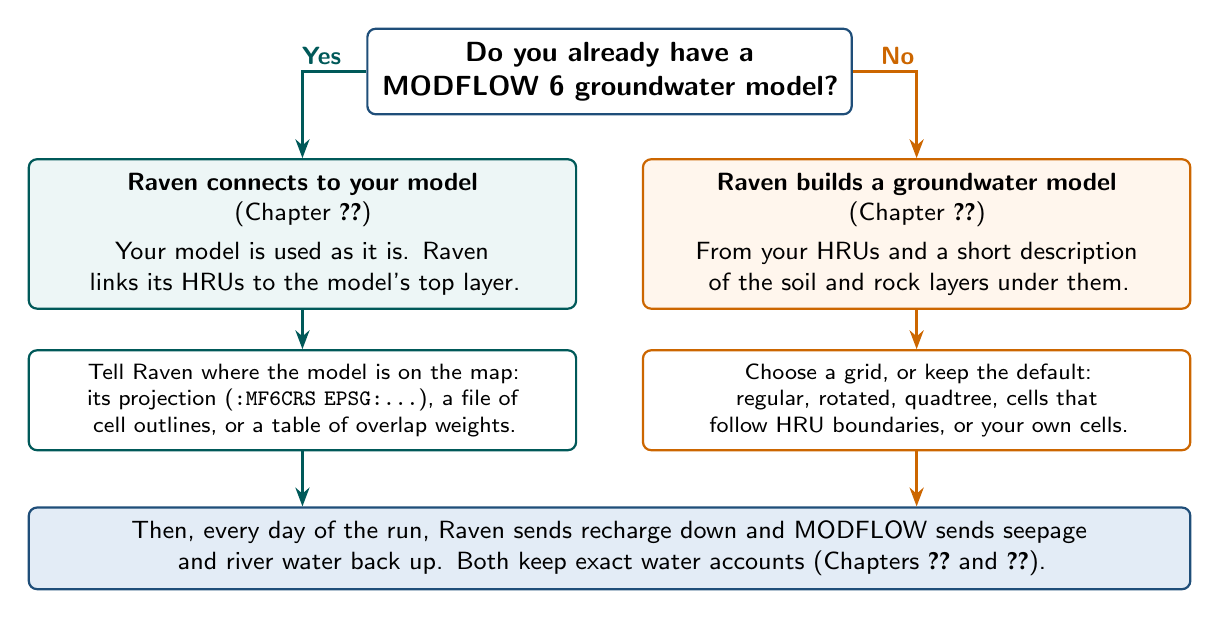
\begin{tikzpicture}[font=\sffamily\small,
  base/.style={rounded corners=3pt,line width=0.8pt,align=center,inner sep=5pt,execute at begin node={\hyphenpenalty=10000\exhyphenpenalty=10000}},
  q/.style={base,draw=brand,fill=white,text width=58mm,font=\sffamily\bfseries},
  yesA/.style={base,draw=teal!70!black,fill=teal!7,text width=66mm},
  noA/.style={base,draw=orange!80!black,fill=orange!7,text width=66mm},
  yesB/.style={base,draw=teal!70!black,fill=white,text width=66mm,font=\sffamily\footnotesize},
  noB/.style={base,draw=orange!80!black,fill=white,text width=66mm,font=\sffamily\footnotesize},
  fin/.style={base,draw=brand,fill=brandlight,text width=144mm},
  arr/.style={-{Stealth[length=2.4mm]},line width=0.9pt},
  lab/.style={font=\sffamily\bfseries\small,inner sep=2pt}]
\node[q] (q) at (0,0) {Do you already have a MODFLOW~6 groundwater model?};
\node[yesA,anchor=north] (y) at (-39mm,-11mm) {\textbf{Raven connects to your model}\\(Chapter~\ref{ch:existing})\\[3pt]Your model is used as it is. Raven links its HRUs to the model's top layer.};
\node[noA,anchor=north] (n) at (39mm,-11mm) {\textbf{Raven builds a groundwater model}\\(Chapter~\ref{ch:c3})\\[3pt]From your HRUs and a short description of the soil and rock layers under them.};
\node[yesB,anchor=north] (y2) at ([yshift=-5mm]y.south) {Tell Raven where the model is on the map: its projection (\texttt{:MF6CRS EPSG:\dots}), a file of cell outlines, or a table of overlap weights.};
\node[noB,anchor=north] (n2) at ([yshift=-5mm]n.south) {Choose a grid, or keep the default: regular, rotated, quadtree, cells that follow HRU boundaries, or your own cells.};
\path let \p1=(y2.south), \p2=(n2.south) in coordinate (m) at (0,{min(\y1,\y2)-7mm});
\node[fin,anchor=north] (e) at (m) {Then, every day of the run, Raven sends recharge down and MODFLOW sends seepage and river water back up. Both keep exact water accounts (Chapters~\ref{ch:c4} and~\ref{ch:c5}).};
\draw[arr,teal!70!black] (q.west) -| node[lab,pos=0.35,above,text=teal!70!black]{Yes} (y.north);
\draw[arr,orange!80!black] (q.east) -| node[lab,pos=0.35,above,text=orange!80!black]{No} (n.north);
\draw[arr,teal!70!black] (y.south) -- (y2.north);
\draw[arr,orange!80!black] (n.south) -- (n2.north);
\draw[arr,teal!70!black] (y2.south) -- (y2.south |- e.north);
\draw[arr,orange!80!black] (n2.south) -- (n2.south |- e.north);
\end{tikzpicture}

\caption{Which chapter to start from: connecting Raven to an existing MODFLOW~6 model, or letting Raven build one.}\label{fig:twoways}
\end{figure}

\section{How to read this manual}
\begin{table}[!htbp]\centering\small
\caption{Where to find what.}\label{tab:readguide}
\begin{tabularx}{\linewidth}{P{0.34\linewidth}Y}\toprule\hdr
If you want to\dots & Read\\\midrule
understand the idea & this chapter and Chapter~\ref{ch:c2} (groundwater in plain terms)\\
connect Raven to your MODFLOW model & Chapter~\ref{ch:existing}; example \cmd{Liard\_existing\_model}\\
let Raven build a groundwater model & Chapter~\ref{ch:c3}; example \cmd{Liard\_groundwater}\\
know what water moves where, and how & Chapters~\ref{ch:c4} and~\ref{ch:c5}\\
look up a command or an output column & Chapter~\ref{ch:c6} and Appendix~\ref{app:tables}\\
set up, calibrate or fix a model & Chapter~\ref{ch:c7}\\
see how the code was tested & Chapter~\ref{ch:c8}\\
change the code & Chapter~\ref{ch:c9}\\\bottomrule
\end{tabularx}
\end{table}
Every chapter starts with a box \emph{In plain words} that says what it covers without technical terms; technical words
are explained in the glossary below.

\section{What the user does --- and what Raven does}
The user works only with Raven's familiar text files:
\begin{enumerate}
\item marks which HRUs have groundwater underneath (\cmd{AQUIFER\_PROFILE} in the \cmd{.rvh} file);
\item describes the aquifer materials and their layering (\cmd{.rvp} file);
\item gives the map of HRUs (a GeoJSON file) and, optionally, land-surface and bedrock maps, rivers, wells,
monitoring wells and boundaries (a new \cmd{.rvg} file);
\item switches the coupling on (\cmd{:GroundwaterModel MODFLOW6} in the \cmd{.rvi} file).
\end{enumerate}
Raven then does everything else automatically: it lays a grid over the HRUs, works out how much of each HRU lies in
each grid cell, builds the layers from the land surface down to bedrock, writes a standard MODFLOW~6 model, starts
MODFLOW, exchanges water every time step, and writes results next to its usual outputs. MODFLOW is used as a
\emph{library} (a program part that another program can call); Raven talks to it through MODFLOW's official
programming interface \cite{hughes2022xmi}. No MODFLOW source code is changed.

\section{Main features}
\begin{itemize}
\item Any number of \emph{aquifer profiles} (layer stacks), each with any number of layers; layer types aquifer,
confined aquifer, aquitard (confining layer) and aquiclude.
\item Land surface and bedrock from raster maps; layers that thin out against bedrock are handled automatically.
\item Coupling to an existing MODFLOW 6 model: Raven links its HRUs to the model's top active layer and leaves the model
      intact, with built-in map projections, unit conversion and safeguards against double counting (Chapter~\ref{ch:existing}).
\item Five grid options: the default regular grid, rotated and refined regular grids, quadtree grids, meshes whose cells
      follow HRU boundaries, and imported cells; layers can be connected by elevation (Section~\ref{sec:gridtypes}).
\item Water exchanges: recharge (with optional delay), groundwater seepage at the land surface, rivers (gaining and
losing), evaporation from a shallow water table, wetlands and lakes held in Raven stores, Raven reservoirs, pumping and
injection wells, head-dependent and fixed-head boundaries.
\item Cells can dry out and rewet; areas of aquifer can disconnect and reconnect by themselves.
\item Monitoring wells: simulated heads are written out and scored against observations like streamflow, so the
groundwater parameters can be calibrated (for example with Ostrich).
\item Hotstart (continuing a run from where another ended), ensembles, NetCDF output of the whole head field.
\item Exact water accounting on both sides, checked automatically by an audit tool supplied with the code.
\end{itemize}

\section{Glossary}
\begin{longtable}{P{0.24\linewidth}P{0.708\linewidth}}
\caption{Glossary.}\\
\toprule\hdr
Term & Meaning\\\midrule\endfirsthead
\caption[]{Glossary (continued).}\\
\toprule\hdr
Term & Meaning\\\midrule\endhead
Active cell & A cell that MODFLOW calculates. Cells outside the aquifer, or switched off in the model, are inactive.\\
API, library & MODFLOW~6 comes as a program library (\cmd{libmf6}) that Raven loads and controls step by step, instead of running it as a separate program.\\
Aquiclude & A layer that, for practical purposes, does not let water through.\\
Aquifer & A soil or rock layer that holds and passes on useful amounts of groundwater (gravel, sand).\\
Aquitard & A layer that lets water through only slowly (clay, till); water leaks through it.\\
Auxiliary variable & An extra column of numbers attached to each entry of a MODFLOW package --- here, for example, the Raven subbasin that a river cell belongs to.\\
Bedrock & The base of the groundwater system in this model; below it no flow is simulated.\\
Cell & One box of the MODFLOW grid. A \emph{column} is the stack of cells at one map location.\\
Conductance & How easily water passes a connection, in m$^2$/d; flow = conductance $\times$ difference in water level.\\
Confined / unconfined & An unconfined aquifer has a free water table; a confined one is completely full and under pressure.\\
Converged & MODFLOW solves each day by repeated improvement; a day has \emph{converged} when the answer stops changing within a small tolerance.\\
Coupled HRU & An HRU that has groundwater underneath it in the model and so exchanges water with MODFLOW.\\
DIS, DISV, DISU & MODFLOW's three ways of describing a grid: rows and columns; layers of any-shaped cells; fully free cells.\\
EPSG code & A standard number for a map projection, e.g.\ EPSG:32610 is UTM zone 10 North. Used with \cmd{:MF6CRS}.\\
Existing-model mode & Using the coupling with a MODFLOW~6 model you already have (Chapter~\ref{ch:existing}).\\
Grid & The set of cells MODFLOW calculates in: squares of one size by default, or other shapes (Section~\ref{sec:gridtypes}).\\
Head ($h$) & The level to which water rises in a well, in metres above sea level. Water flows from high to low head.\\
Hotstart, restart & Starting a run from the saved end state (\cmd{solution.rvc}) of an earlier run, so a long run can be split or continued.\\
HRU & Hydrologic Response Unit: Raven's basic land unit, an area that behaves alike.\\
Hydraulic conductivity ($K$) & How easily water moves through a material, in m/d.\\
Leakance & How easily water passes a thin layer (a riverbed, the ground surface), per square metre, in 1/d.\\
Linkage, overlap & How much of each HRU lies in each grid cell. It decides where each HRU's water goes.\\
Newton method & The way MODFLOW solves its equations here; it copes well with cells drying out and filling up again.\\
Overlap weight & The share of a cell covered by an HRU (0 to 1); a table of them can replace the map of cells (\cmd{:OverlapWeights}).\\
Package & One component of a MODFLOW model, in its own file: wells (WEL), rivers (RIV), recharge (RCH) and so on.\\
Pass-through cell & A very thin cell where a layer is missing; water passes straight through it from the layer above to the layer below.\\
Profile & A stack of aquifer layers assigned to HRUs (used when Raven builds the model).\\
Projection & The rule that turns positions on the round Earth into flat map coordinates in metres; MODFLOW models use one, usually without saying which.\\
Quadtree, mesh & Grids with cells of different sizes: a quadtree cuts squares into four where detail is wanted; a mesh (here) has cells shaped to follow HRU boundaries.\\
Recharge & Water that reaches the water table from above.\\
Seepage & Groundwater flowing out at the land surface where the water table reaches it.\\
Specific storage ($S_s$) & Water released per m$^3$ of aquifer per metre of head fall when the aquifer stays full [1/m].\\
Specific yield ($S_y$) & Water released per m$^2$ of water table per metre of fall when the aquifer drains [--].\\
Stage & Water level in a river, lake or reservoir [m].\\
Steady state & A calculation as if conditions never changed --- the long-term balance. Often used for the first period of a model.\\
Stress period & A stretch of time in a MODFLOW model (often a month) during which inputs such as pumping rates stay the same.\\
Time step & One step of the calculation; in the coupling, one Raven time step (usually a day).\\
Transmissivity ($T$) & $K$ times saturated thickness, in m$^2$/d.\\
Water table & The top of the saturated zone in an unconfined aquifer.\\
Working copy & The copy of an existing MODFLOW model that Raven runs, in \cmd{output/mf6/}; your own files are never changed.\\
XT3D & An optional, more exact way for MODFLOW to calculate flow between cells of odd shapes; slower and off by default.\\\bottomrule
\end{longtable}

\section{The big picture}\label{ch:overview}
\subsection{Who owns which water}
Every drop of water in the coupled system belongs to exactly one of the two models at any time:
\begin{itemize}
\item \textbf{Raven} owns snow, canopy, soil and vadose-zone stores, depressions and wetlands, rivers, lakes and
reservoirs.
\item \textbf{MODFLOW} owns the saturated groundwater below the \emph{model top}. By default the model top is the land
surface (as in GSFLOW \cite{markstrom2008gsflow}); users with physically based soil layers can lower it with
\cmd{SOIL\_ZONE\_DEPTH}.
\end{itemize}
Water moves between the two only through the exchanges described in Chapter~\ref{ch:c4}, and each exchange is recorded on both
sides. In a coupled HRU, Raven's \cmd{GROUNDWATER} store is a \emph{pass-through}: whatever enters it during a day is
handed to MODFLOW as recharge that day.

\subsection{The pieces of the software}
Figure~\ref{fig:arch} shows the parts. The \emph{model builder} runs once at the start: it reads the inputs and writes a
standard MODFLOW~6 model. The \emph{exchange} runs every time step.

\begin{figure}[!htbp]\centering
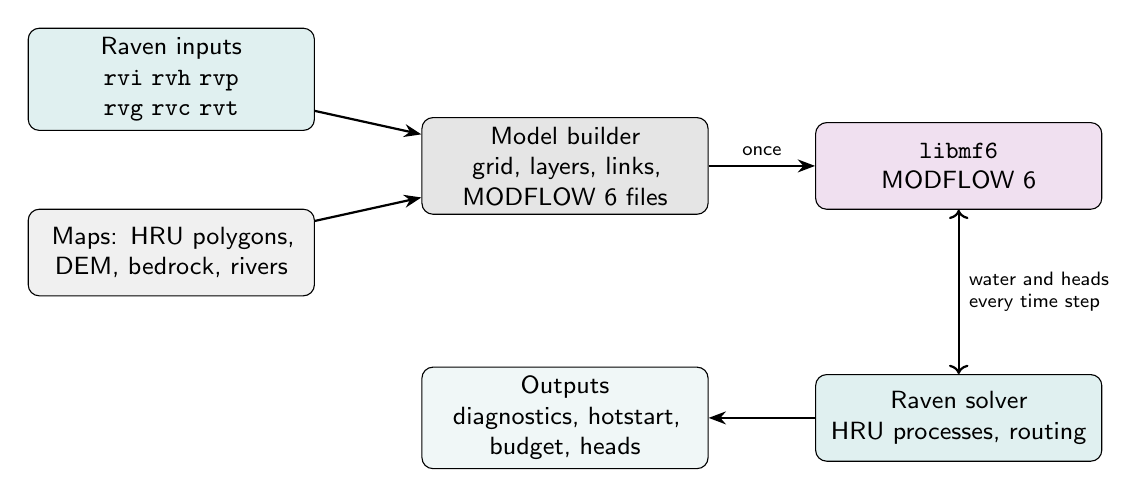
\begin{tikzpicture}[box/.style={draw,rounded corners,align=center,minimum height=11mm,text width=34mm,font=\small},
 ar/.style={-{Stealth[length=2.2mm]},thick}]
\node[box,fill=teal!12] (in) at (0,1.1) {Raven inputs\\ \cmd{rvi rvh rvp rvg rvc rvt}};
\node[box,fill=gray!12] (geo) at (0,-1.1) {Maps: HRU polygons, DEM, bedrock, rivers};
\node[box,fill=gray!20] (bld) at (5,0) {Model builder\\ grid, layers, links,\\ MODFLOW 6 files};
\node[box,fill=violet!12] (mf) at (10,0) {\cmd{libmf6}\\ MODFLOW 6};
\node[box,fill=teal!12] (rv) at (10,-3.2) {Raven solver\\ HRU processes, routing};
\node[box,fill=teal!6] (out) at (5,-3.2) {Outputs\\ diagnostics, hotstart,\\ budget, heads};
\draw[ar] (in) -- (bld); \draw[ar] (geo) -- (bld);
\draw[ar] (bld) -- node[above,font=\scriptsize]{once} (mf);
\draw[ar,<->] (mf) -- node[right,font=\scriptsize,align=left]{water and heads\\ every time step} (rv);
\draw[ar] (rv) -- (out);
\end{tikzpicture}
\caption{The software pieces. The builder runs once per simulation (or per ensemble member); the exchange runs every
time step.}\label{fig:arch}
\end{figure}

\subsection{One day in the life of the coupled model}
The following happens every time step (one day in the examples); Section~\ref{ch:timestep} gives the exact algorithm.
\begin{enumerate}
\item \textbf{Raven's land-surface day.} Raven calculates snowmelt, infiltration, evaporation and flow between its soil
layers. In coupled HRUs, water that percolates past the soil ends up in \cmd{GROUNDWATER}.
\item \textbf{Recharge handed over.} The water in each HRU's \cmd{GROUNDWATER} is spread over the grid cells under that
HRU, in proportion to how much of the HRU lies in each cell.
\item \textbf{Stresses set.} River levels (from Raven's rivers at the start of the day), well pumping rates,
boundary heads, wetland and lake levels, and the evaporation demand not met by Raven are passed to MODFLOW.
\item \textbf{MODFLOW's day.} MODFLOW calculates new heads everywhere, including the flows to and from rivers,
drains, wells and boundaries.
\item \textbf{Water handed back.} Groundwater that seeps out at the land surface is added to a Raven store of the HRUs
above; groundwater that discharges to rivers is added to the river inflow of the subbasin; river losses are taken from
the river; wetland and lake exchanges change those Raven stores.
\item \textbf{Raven's river day.} Raven routes water down the river network, now including the groundwater
contributions. Reservoirs compute their seepage using the aquifer head beneath them.
\item \textbf{Accounts.} Both models update their water balances, and the groundwater outputs are written.
\end{enumerate}

\subsection{Design principles}
\begin{enumerate}
\item \textbf{Raven is the single user interface.} All inputs are Raven files; MODFLOW files are generated.
\item \textbf{Standard MODFLOW only.} Only standard MODFLOW~6 packages are used; the generated model can be opened in
FloPy or ModelMuse.
\item \textbf{Each fact is entered once.} Geometry comes from maps, hydrogeology from profiles, time-varying stresses
from time series.
\item \textbf{Generic.} Nothing is specific to a basin; any Raven model can couple any subset of its HRUs.
\item \textbf{Exact accounting.} Every exchanged volume is computed once and applied identically on both sides.
\item \textbf{No surprise for existing users.} Models without groundwater give bit-for-bit the same results as
Raven~4.15 (the version this coupling is built on); Raven still builds and runs without MODFLOW installed.
\end{enumerate}

\section{Scope and assumptions}
\begin{itemize}
\item \textbf{What is simulated by MODFLOW:} saturated groundwater flow (Darcy flow, storage change) in a layered aquifer
system under the coupled HRUs, including dry and rewetting cells.
\item \textbf{What stays in Raven:} everything above the model top --- snow, canopy, soil and unsaturated zone, surface
runoff, depressions, rivers, lakes and reservoirs --- and all HRUs without an aquifer profile.
\item \textbf{Water density and temperature} are constant; there is no salt-water or heat transport.
\item \textbf{The grid} is regular (square cells); the model area is the part of the rectangle around the coupled HRUs
that those HRUs cover.
\item \textbf{Time}: both models use Raven's time step (daily or shorter). Exchanges are explicit between the models at
the step level, but every head-dependent exchange is implicit inside MODFLOW.
\end{itemize}

\section{When to use the coupling --- and when not to}
Use it when the question involves the \emph{spatial} behaviour of groundwater: water-table depth at a location, effects of
pumping on streams, gaining and losing reaches, groundwater flow between subbasins, wetlands fed by groundwater, drought
recession of large aquifers, or when head measurements should constrain the model. Raven's conceptual baseflow remains the
better choice for fast screening, very large ensembles, or basins without a significant aquifer.

\section{What changes for an existing Raven model}
\begin{itemize}
\item Nothing, unless \cmd{:GroundwaterModel MODFLOW6} is added: results stay bit-for-bit identical.
\item With the coupling on, coupled HRUs lose their conceptual deep-groundwater behaviour (their \cmd{GROUNDWATER} store
becomes a pass-through), and their baseflow now comes from the aquifer via seepage and river exchange.
\item Run times increase: the 20-year Liard run (3\,252 active columns) takes about 15 minutes instead of 35 seconds on one processor core.
\end{itemize}

\section{Files at a glance}
\begin{table}[!htbp]\centering
\caption{Input and output files of the coupling.}
\begin{tabular}{P{0.2\linewidth}P{0.748\linewidth}}\toprule\hdr
File & Role in the coupling\\\midrule
\cmd{.rvi} & switch on (\cmd{:GroundwaterModel MODFLOW6}); route recharge into \cmd{GROUNDWATER}\\
\cmd{.rvh} & \cmd{AQUIFER\_PROFILE} per HRU; reservoirs with \cmd{:SeepageParameters}\\
\cmd{.rvp} & aquifer classes, profiles and profile parameters\\
\cmd{.rvg} & geometry (HRU polygons, maps, rivers), grid, wells, monitoring wells, boundaries, options\\
\cmd{.rvt} & well rates, boundary heads, observed heads\\
\cmd{.rvc} & initial heads; hotstart blocks written by Raven\\
GeoJSON, ASCII grids & HRU polygons, river lines, boundary shapes; DEM and bedrock maps\\
\cmd{<output>/mf6/} & generated MODFLOW 6 model and its own outputs\\\bottomrule
\end{tabular}
\end{table}

\chapter{Groundwater concepts}\label{ch:c2}\label{ch:concepts}
This chapter introduces the physical ideas and vocabulary used in the rest of the document. Readers familiar with
groundwater hydrology can skim it; everyone else will find every later equation built from the few ideas presented here.


\section{Head}
The \emph{head} $h$ at a point is the elevation to which water would rise in a small well drilled to that point, in
metres above a common datum (here, the same datum as the digital elevation model). Groundwater always flows from
higher head to lower head. In an unconfined aquifer the head is the elevation of the water table; the \emph{depth to
water} is land-surface elevation minus head.

\section{Darcy's law}
The flow of water through a porous material is proportional to the drop in head and to the cross-section, and
inversely proportional to the distance travelled:
\begin{equation}
Q = K\,A\,\frac{h_1-h_2}{L},
\end{equation}
where $Q$ is the flow [m$^3$/d], $K$ the hydraulic conductivity [m/d], $A$ the area the water passes through [m$^2$],
$h_1-h_2$ the head difference [m] and $L$ the distance [m].

\begin{example}[: Darcy's law]
Gravel with $K=50$ m/d, a 2\,000 m wide and 10 m thick strip ($A=20\,000$ m$^2$), heads 101 m and 100 m, 2\,000 m apart:
$Q=50\times20\,000\times1/2\,000=500$ m$^3$/d.
\end{example}

\section{Transmissivity and conductance}
Because $K$, $A$ and $L$ always appear together, it is convenient to combine them into a \emph{conductance}
$C = K A/L$ [m$^2$/d], so that $Q=C\,(h_1-h_2)$. Every exchange in this document --- between two grid cells, between an
aquifer and a river, a drain, a wetland --- is written in this form: \textbf{flow = conductance $\times$ head
difference}. For a layer of saturated thickness $b$, the \emph{transmissivity} is $T=Kb$ [m$^2$/d].

Between two neighbouring cells with different conductivities $K_1,K_2$, the conductance is the series combination
(harmonic mean), because water must pass through both halves in turn:
\begin{equation}
C_{12}=\frac{1}{\dfrac{L_1}{K_1A}+\dfrac{L_2}{K_2A}} .
\end{equation}
\begin{example}[: harmonic mean]
Two 2\,000 m cells, 10 m thick and 2\,000 m wide ($A=20\,000$ m$^2$, $L_1=L_2=1\,000$ m to the shared face), gravel
$K_1=50$ m/d next to till $K_2=0.2$ m/d:
$C_{12}=1/(1\,000/(50\cdot20\,000)+1\,000/(0.2\cdot20\,000)) = 1/(0.001+0.25)=3.98$ m$^2$/d. The low-conductivity
material controls the flow.
\end{example}

\section{Storage}
When the head in an aquifer falls, water is released from storage.
\begin{itemize}
\item In an \emph{unconfined} aquifer the water table drops and pores drain. The water released per square metre per
metre of fall is the \emph{specific yield} $S_y$ (typically 0.05--0.30).
\item In a \emph{confined} (full) aquifer, water is released only by the slight expansion of water and compression of
the grains; per cubic metre of aquifer per metre of head fall this is the \emph{specific storage} $S_s$
(typically $10^{-6}$--$10^{-4}$ 1/m).
\end{itemize}
\begin{example}[: storage change]
A 4 km$^2$ cell of gravel ($S_y=0.25$) whose water table falls 0.1 m in a day releases
$4\times10^6\times0.25\times0.1=100\,000$ m$^3$. The same fall in a 20 m thick confined sand ($S_s=10^{-5}$ 1/m)
releases $4\times10^6\times20\times10^{-5}\times0.1=80$ m$^3$ --- over a thousand times less.
\end{example}

\section{The groundwater flow equation}
Combining Darcy's law with conservation of water (what flows in, minus what flows out, equals the change in storage)
gives the equation MODFLOW solves. For one cell $n$ with neighbours $m$:
\begin{equation}
\sum_{m}C_{nm}\left(h_m-h_n\right) + \sum_{b}q_{b,n} = S_n\,\frac{h_n^{\,t+\dt}-h_n^{\,t}}{\dt},
\end{equation}
where all heads are those at the end of the step, $t+\dt$ (MODFLOW's implicit scheme, which is stable for any step
length), the first sum is flow from the neighbours, $q_{b,n}$ are the boundary flows of the cell (recharge, rivers,
drains, wells, \dots; positive into the aquifer), and $S_n$ is the storage capacity of the cell ($S_y$ times area when
unconfined, $S_s$ times volume when confined). Writing this for every cell gives a large set of equations for the
unknown heads, which MODFLOW solves every time step.

\begin{plain}
Each cell is a small water account: inflows from neighbours and boundaries, minus outflows, equals the change of water
stored. MODFLOW finds the heads that make every cell's account balance at the same time.
\end{plain}

\section{Head-dependent boundaries}
Many exchanges depend on the head: a river gives water to the aquifer when the river is higher than the water table,
and receives water when it is lower. MODFLOW writes such a boundary as
\begin{equation}
q_b = C_b\left(h_b-h_n\right),
\end{equation}
where $h_b$ is the boundary's water level. Because $q_b$ depends on the unknown head $h_n$, MODFLOW solves for the
boundary flow together with the heads; this keeps the solution stable even with large conductances. In MODFLOW's
internal notation each boundary contributes two numbers per cell, HCOF and RHS, and its flow is
\begin{equation}
q_b = \mathrm{HCOF}\cdot h_n-\mathrm{RHS}.
\end{equation}
The coupling uses exactly this formula, with MODFLOW's own HCOF and RHS, to compute every exchanged flow. It is the same
formula MODFLOW uses for its own budget, so the numbers exchanged with Raven are exactly the numbers MODFLOW accounts for.

\section{Water table and potentiometric surface}
In an unconfined aquifer the head is the water-table elevation and the pores above it are partly empty. In a confined
aquifer, sealed above by a low-permeability layer, water rises in a well above the top of the aquifer; the imaginary
surface joining these levels is the \emph{potentiometric surface}. The same aquifer can be confined in one place and
unconfined in another, or change over time as heads fall; MODFLOW's \emph{convertible} layers handle this switch
automatically by using $S_s$ while full and $S_y$ once the head falls below the top of the layer.

\begin{figure}[!htbp]\centering
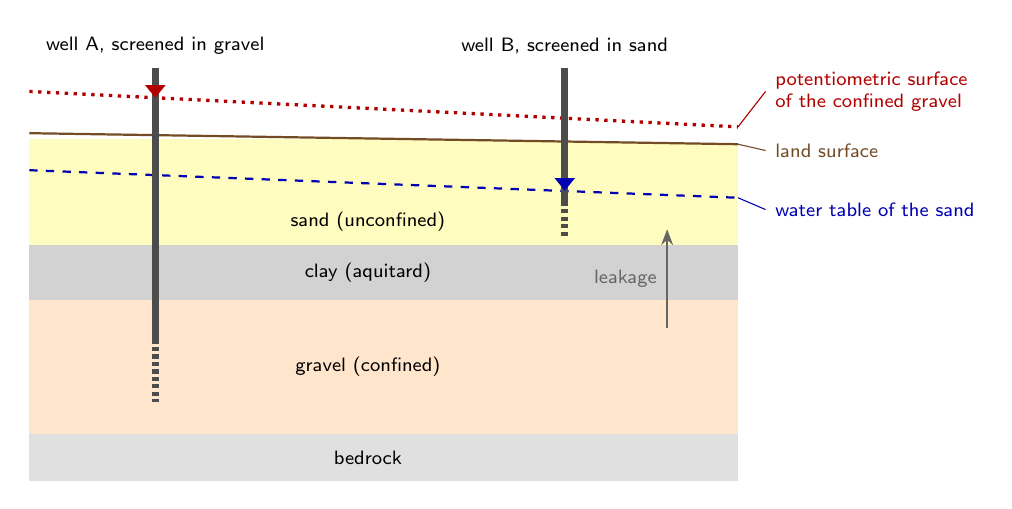
\begin{tikzpicture}[x=1cm,y=1cm,lab/.style={font=\scriptsize,align=center},leg/.style={font=\scriptsize,anchor=west,align=left}]
\fill[yellow!25] (0,3) rectangle (9,4.35); \fill[gray!35] (0,2.3) rectangle (9,3);
\fill[orange!20] (0,0.6) rectangle (9,2.3); \fill[black!12] (0,0) rectangle (9,0.6);
\fill[white] (0,4.42) -- (9,4.28) -- (9,4.4) -- (0,4.5) -- cycle;
\draw[thick,brown!60!black] (0,4.42) -- (9,4.28);
\draw[dotted,red!70!black,very thick] (0,4.95) -- (9,4.5);
\draw[dashed,blue!70!black,thick] (0,3.95) -- (9,3.6);
\node[lab] at (4.3,3.3) {sand (unconfined)}; \node[lab] at (4.3,2.65) {clay (aquitard)};
\node[lab] at (4.3,1.45) {gravel (confined)}; \node[lab] at (4.3,0.3) {bedrock};
\draw[line width=2.5pt,black!70] (1.6,5.25) -- (1.6,1.8); \draw[line width=2.5pt,black!70,dash pattern=on 1.5pt off 1.2pt] (1.6,1.8) -- (1.6,1.0);
\fill[red!70!black] (1.6,4.87) -- ++(-0.13,0.16) -- ++(0.26,0) -- cycle;
\node[lab,anchor=south] at (1.6,5.3) {well A, screened in gravel};
\draw[line width=2.5pt,black!70] (6.8,5.25) -- (6.8,3.55); \draw[line width=2.5pt,black!70,dash pattern=on 1.5pt off 1.2pt] (6.8,3.55) -- (6.8,3.1);
\fill[blue!70!black] (6.8,3.69) -- ++(-0.13,0.16) -- ++(0.26,0) -- cycle;
\node[lab,anchor=south] at (6.8,5.3) {well B, screened in sand};
\draw[-{Stealth[length=2mm]},thick,black!60] (8.1,1.95) -- node[lab,left]{leakage} (8.1,3.2);
\draw[red!70!black] (9,4.5) -- (9.35,4.95) node[leg] {potentiometric surface\\ of the confined gravel};
\draw[brown!60!black] (9,4.28) -- (9.35,4.2) node[leg] {land surface};
\draw[blue!70!black] (9,3.6) -- (9.35,3.45) node[leg] {water table of the sand};
\end{tikzpicture}
\caption{The same place can have two different heads: the water table of the upper sand and the higher potentiometric surface of
the confined gravel below the clay. Water leaks upward through the clay because the gravel head is higher.}\label{fig:potsurf}
\end{figure}
\section{Three kinds of boundary conditions}
\begin{table}[!htbp]\centering
\caption{Three kinds of boundary conditions.}
\begin{tabular}{P{0.22\linewidth}P{0.368\linewidth}P{0.34\linewidth}}\toprule\hdr
Kind & Meaning & In this coupling\\\midrule
Specified flow & the flow is known (it does not depend on the head) & recharge, wells, reservoir seepage\\
Specified head & the head is known; the flow is whatever is needed & fixed-head boundaries (CHD)\\
Head-dependent flow & flow = conductance $\times$ (boundary level $-$ head) & rivers, seepage drains, wetlands, lakes, general-head boundaries, water-table ET\\\bottomrule
\end{tabular}
\end{table}
Head-dependent boundaries are the heart of a coupled model: they let the aquifer and the surface water ``negotiate'' the
exchange according to the water levels on both sides.

\section{The Newton method in simple terms}
The flow equations are non-linear: in an unconfined layer, transmissivity depends on the saturated thickness, which
depends on the unknown head. MODFLOW therefore solves them iteratively: guess heads, compute the imbalance of every cell,
correct the heads, and repeat until the corrections are smaller than a tolerance (here 0.00001 m, i.e.\ 0.01 mm). The Newton--Raphson method
computes each correction from the slope of the imbalance with respect to the heads, which converges quickly even when cells
are nearly dry. Each repetition is an \emph{outer iteration}; \cmd{GWBudget.csv} reports how many were needed each step
(typically 3--10 in the Liard example).

\section{A cell's water account, with numbers}
\begin{example}[: one cell for one day]
A 4 km$^2$ gravel cell receives 8\,000 m$^3$ recharge; it gets 1\,500 m$^3$ from an up-gradient neighbour and passes
2\,500 m$^3$ to a down-gradient one; its drain removes 4\,000 m$^3$. Inflow $-$ outflow $=8\,000+1\,500-2\,500-4\,000=3\,000$
m$^3$ are stored, so with $S_y=0.25$ the water table rises by $3\,000/(4\times10^6\times0.25)=3$ mm. MODFLOW finds heads for
which every cell's account balances like this one at the same time.
\end{example}

\section{Units and conversions}
\begin{table}[!htbp]\centering
\caption{Units and conversions.}
\begin{tabular}{P{0.44\linewidth}P{0.5\linewidth}}\toprule\hdr
Quantity & Conversion\\\midrule
depth of water in an HRU to volume & $V\,[\mathrm{m}^3]=x\,[\mathrm{mm}]\times A\,[\mathrm{km}^2]\times1000$\\
flow & 1 m$^3$/s $=86\,400$ m$^3$/d\\
recharge rate & 1 mm/d over 1 km$^2$ $=1\,000$ m$^3$/d\\
hydraulic conductivity & 1 m/d $\approx1.16\times10^{-5}$ m/s\\
leakance & conductance per area, d$^{-1}$; $C=L\times$area\\\bottomrule
\end{tabular}
\end{table}

\chapter{Building the groundwater model}\label{ch:c3}
Raven's HRUs are irregular areas; MODFLOW needs a regular three-dimensional grid. This chapter follows the model builder step by step. It shows which HRUs are coupled, how their polygons are placed on a map
and covered with a grid, and how much of each HRU falls in each cell. It then shows how the layers are built from the land
surface down to bedrock, which MODFLOW files are written, and how MODFLOW solves each step.

\section{From HRUs to a groundwater grid}\label{ch:grid}
\subsection{Which HRUs are coupled}
An HRU is \emph{coupled} when its \cmd{AQUIFER\_PROFILE} in the \cmd{.rvh} file names a profile defined in the
\cmd{.rvp} file. HRUs with \cmd{[NONE]} (or an empty entry) keep Raven's usual behaviour. Disabled HRUs are never
coupled (Raven prints a warning). We write $\mathcal{K}$ for the set of coupled HRUs and $p(k)$ for the profile of HRU $k$.

Raven checks two rules at start-up:
\begin{itemize}
\item No Raven process may take water \emph{out of} \cmd{GROUNDWATER} in a coupled HRU (MODFLOW owns that water);
Raven stops with an error naming the process.
\item If a process sends water \emph{into} \cmd{GROUNDWATER} in an \emph{uncoupled} HRU, that water leaves the model;
Raven warns so the user can restrict the process with \cmd{:-->Conditional}.
\end{itemize}

\subsection{Map projection}
The HRU polygons are read from a GeoJSON file. GeoJSON coordinates are longitude $\lambda$ and latitude $\phi$ in
degrees, which cannot be used directly for areas and distances. Raven converts them to metres with the
\emph{Lambert azimuthal equal-area} projection \cite{snyder1987map}, centred on the average centroid
$(\lambda_0,\phi_0)$ of the coupled HRUs, on a sphere of radius $R=6\,371\,007.181$ m:
\begin{align}
k' &= \sqrt{\frac{2}{1+\sin\phi_0\sin\phi+\cos\phi_0\cos\phi\cos(\lambda-\lambda_0)}},\\
x &= R\,k'\cos\phi\,\sin(\lambda-\lambda_0),\\
y &= R\,k'\left[\cos\phi_0\sin\phi-\sin\phi_0\cos\phi\cos(\lambda-\lambda_0)\right].
\end{align}
The reverse conversion (used to look up map values at cell locations) is
\begin{align}
\rho&=\sqrt{x^2+y^2},\qquad c=2\arcsin\frac{\rho}{2R},\\
\phi&=\arcsin\!\left(\cos c\sin\phi_0+\frac{y\sin c\cos\phi_0}{\rho}\right),\\
\lambda&=\lambda_0+\operatorname{atan2}\!\left(x\sin c,\;\rho\cos\phi_0\cos c-y\sin\phi_0\sin c\right).
\end{align}
\begin{plain}
This projection keeps areas correct, which is what matters for water volumes: one square kilometre on the map is one
square kilometre on the ground, anywhere in the model area.
\end{plain}

\subsection{The grid}
By default a square grid with cell size $\Delta$ (\cmd{:GridCellSize}, default 1\,000 m) covers the rectangle around all
coupled HRUs. Rows are numbered from north to south and columns from west to east. The plan-view cell (a whole column of
layers) is indexed $i$; its lower-left corner is $(x_0+c\Delta,\;y_0+(n_r-1-r)\Delta)$ for row $r$ and column $c$. Rotated
grids, grids refined around rivers and wells, quadtree grids, meshes that follow HRU boundaries and imported cells are
described in Section~\ref{sec:gridtypes}; everything below applies to all of them, with cell $i$ a polygon of area $A_i$.

\subsection{Polygon areas}
The area of a polygon with corners $(x_1,y_1),\dots,(x_n,y_n)$ is given by the shoelace formula
\begin{equation}
A=\tfrac12\sum_{j=1}^{n}\left(x_jy_{j+1}-x_{j+1}y_j\right),\qquad (x_{n+1},y_{n+1})=(x_1,y_1).
\end{equation}
The result is positive when the corners run counter-clockwise. Raven orients outer boundaries counter-clockwise and
holes clockwise, so the area of a polygon with holes is simply the sum over all its rings.
\begin{example}[: shoelace formula]
A square from $(0,0)$ to $(2,2)$ km: $\tfrac12[(0\cdot0-2\cdot0)+(2\cdot2-2\cdot0)+(2\cdot2-0\cdot2)+(0\cdot0-0\cdot2)]=\tfrac12(0+4+4+0)=4$ km$^2$.
\end{example}

\subsection{How much of each HRU lies in each cell}\label{sec:linkage}
For every HRU polygon $P_k$ and every cell $\Omega_i$ it touches, Raven cuts the polygon to the cell rectangle with
the Sutherland--Hodgman clipping algorithm \cite{sutherland1974clip} and measures the area of what remains:
\begin{equation}
A_{k,i}=\left|P_k\cap\Omega_i\right| .
\end{equation}
For rectangular cells (regular and quadtree grids) the polygon is clipped by the cell rectangle; for convex cells (HRU
meshes) by the cell polygon; a concave imported cell is split into triangles and clipped by each. The clipping works one
cell edge at a time: walking around the polygon, it keeps the corners that are inside the edge
and adds a new corner wherever the polygon crosses the edge. After four edges, what is left is the part of the polygon
inside the cell; the shoelace formula gives its area. (This gives the correct area even for concave polygons.)

\begin{example}[: overlap areas]
An HRU of 10 km$^2$ lies over three 2~km cells, covering 4.0, 3.5 and 2.5 km$^2$ of them. Its overlaps are
$A_{k,1}=4.0$, $A_{k,2}=3.5$, $A_{k,3}=2.5$ km$^2$, and the fractions of the HRU in each cell are 0.40, 0.35 and 0.25.
Every flow from this HRU to the grid is split 40/35/25.
\end{example}

\subsection{Active cells and their profile}
A column is \emph{active} when the coupled HRUs cover at least a fraction $f_{\min}$ (\cmd{:MinCellCoverage}, default
0.25) of it:
\begin{equation}
a_i=\sum_{k\in\mathcal{K}}A_{k,i}\ \ge\ f_{\min}\,\Delta^2 .
\end{equation}
An active column takes the profile of the HRU with the largest overlap (the \emph{dominant} HRU),
$p(i)=p\!\left(\arg\max_k A_{k,i}\right)$. Fluxes still use the exact overlaps, so a column shared by two HRUs receives
water from both.

The table of overlaps $A_{k,i}$ over active columns is called the \emph{linkage}. It is the single source of truth for
moving water between HRUs and cells in both directions (Sections~\ref{ch:recharge}--\ref{ch:stores}).

\begin{watch}
The polygon area of an HRU need not equal its \cmd{AREA} in the \cmd{.rvh} file (Raven prints a warning when they
differ by more than 5\%). This does not break the water balance: volumes are always computed from the \cmd{.rvh} area
and split by overlap \emph{fractions}.
\end{watch}

\subsection{The linkage cache}
Computing the linkage requires reading and clipping every polygon. The result is saved in \cmd{<output>/mf6/linkage.cache}
(or the file named by \cmd{:LinkageCache}). The cache is labelled with a fingerprint (an FNV-1a hash) of the GeoJSON
file together with the ID field, the cell size and the list of coupled HRUs; if any of these change, Raven recomputes
the linkage. Numbers are written with 17 significant digits, so a run that reads the cache gives exactly the same
results as one that computed it.

\begin{figure}[!htbp]\centering
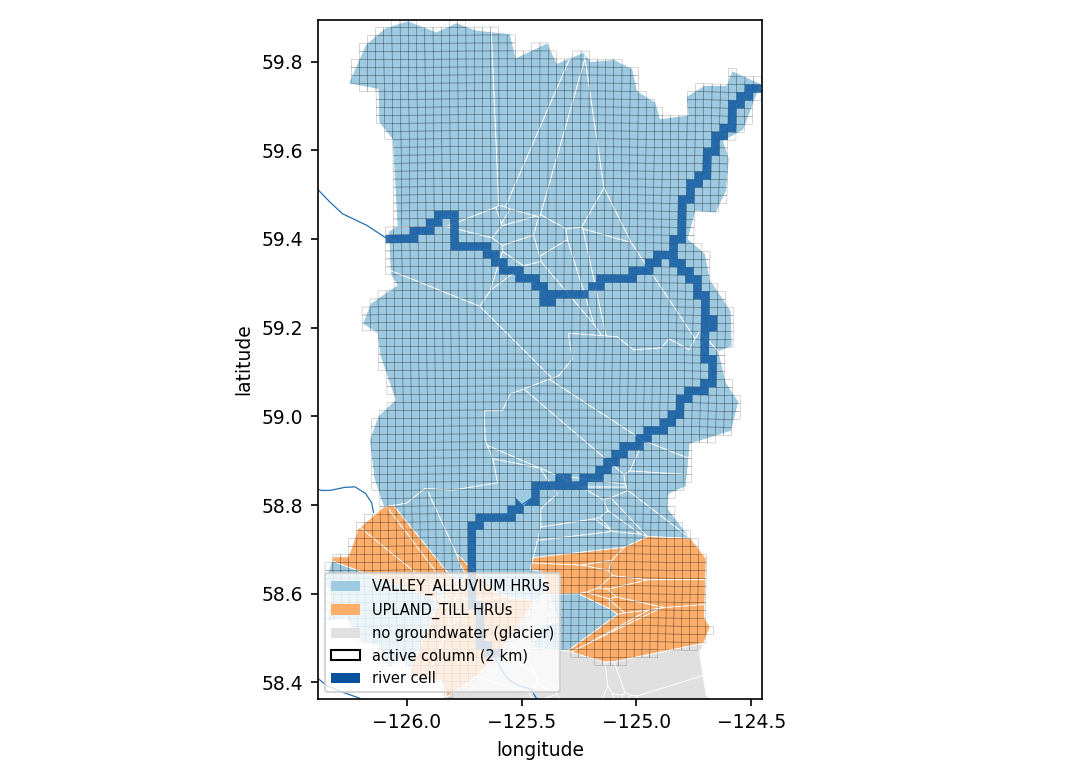
\includegraphics[width=0.9\linewidth]{figures/fig_grid_liard.png}
\caption{Liard example: coupled HRUs (colour = aquifer profile), active 2~km columns and river cells.}\label{fig:grid}
\end{figure}

\section{From one HRU to its cells: a complete example}
\begin{figure}[!htbp]\centering
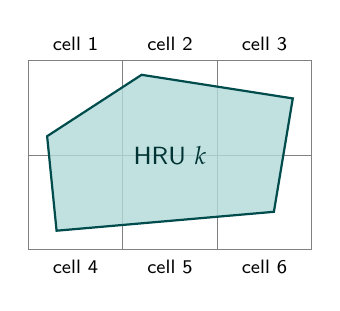
\begin{tikzpicture}[x=1.2cm,y=1.2cm]
\foreach \x in {0,1,2,3} \draw[gray] (\x,0) -- (\x,2);
\foreach \y in {0,1,2} \draw[gray] (0,\y) -- (3,\y);
\fill[teal!30,opacity=0.8] (0.3,0.2) -- (2.6,0.4) -- (2.8,1.6) -- (1.2,1.85) -- (0.2,1.2) -- cycle;
\draw[teal!60!black,thick] (0.3,0.2) -- (2.6,0.4) -- (2.8,1.6) -- (1.2,1.85) -- (0.2,1.2) -- cycle;
\node[font=\scriptsize] at (0.5,2.18) {cell 1}; \node[font=\scriptsize] at (1.5,2.18) {cell 2}; \node[font=\scriptsize] at (2.5,2.18) {cell 3};
\node[font=\scriptsize] at (0.5,-0.18) {cell 4}; \node[font=\scriptsize] at (1.5,-0.18) {cell 5}; \node[font=\scriptsize] at (2.5,-0.18) {cell 6};
\node[font=\small,teal!40!black] at (1.5,1.0) {HRU $k$};
\end{tikzpicture}
\caption{An HRU polygon over six grid cells. Clipping gives its area in each cell.}\label{fig:hrucells}
\end{figure}
\begin{example}[: an HRU through the whole chain]
Suppose the HRU in Figure~\ref{fig:hrucells} has an \cmd{.rvh} area of 3.2 km$^2$, 2 km cells, and clipping gives overlaps (km$^2$)
0.45, 0.55, 0.30 in cells 1--3 and 0.60, 0.85, 0.45 in cells 4--6 (sum 3.20).
\begin{enumerate}
\item \emph{Activation.} If other coupled HRUs fill the rest of these cells, all six have coverage above 25\% and are active.
\item \emph{Recharge.} Raven's percolation puts 1.5 mm into \cmd{GROUNDWATER}: $V=0.0015\times3.2\times10^6=4\,800$ m$^3$.
Cell 5 receives $4\,800\times0.85/3.20=1\,275$ m$^3$, i.e.\ $1\,275/4\times10^6=0.32$ mm over the whole cell (plus whatever other
HRUs deliver).
\item \emph{Seepage back.} If cell 5 seeps 10\,000 m$^3$ in the day and our HRU covers 0.85 of the 4 km$^2$ covered by all
HRUs in that cell, the HRU receives $10\,000\times0.85/4.0=2\,125$ m$^3$, i.e.\ $2\,125/3.2\times10^6\times1000=0.66$ mm in its lowest soil layer.
\item \emph{Water-table depth in the outputs.} \cmd{GWHRUState.csv} reports the overlap-weighted mean head of the six cells.
\end{enumerate}
\end{example}

\section{Preparing the geometry}
\subsection{What the HRU GeoJSON must contain}
A \cmd{FeatureCollection} of \cmd{Polygon} or \cmd{MultiPolygon} features in longitude/latitude (EPSG:4326), each with a
property holding the HRU ID of the \cmd{.rvh} file. Holes are allowed. Several features may share an ID (their areas add up).
\par\noindent\begin{minipage}{\linewidth}
\begin{lstlisting}
{"type":"FeatureCollection","features":[
 {"type":"Feature","properties":{"HRU_ID":2736},
  "geometry":{"type":"Polygon","coordinates":[[[-124.91,59.22],[-124.80,59.22],
              [-124.80,59.30],[-124.91,59.30],[-124.91,59.22]]]}} ]}
\end{lstlisting}
\end{minipage}\par\smallskip
Only HRUs with an \cmd{AQUIFER\_PROFILE} need polygons; others may be present and are ignored.
\subsection{Raster maps}
ESRI ASCII grids in longitude/latitude, for example:
\par\noindent\begin{minipage}{\linewidth}
\begin{lstlisting}
ncols 125
nrows 115
xllcorner -126.6
yllcorner 58.1
cellsize 0.02
NODATA_value -9999
 612.3 615.9 ...
\end{lstlisting}
\end{minipage}\par\smallskip
Values are interpolated bilinearly between raster cell centres, ignoring no-data cells; each model cell takes the mean of
$5\times5$ such samples. Points more than one raster cell outside the map count as no-data.
\subsection{Choosing the cell size}
The number of active columns is roughly the coupled area divided by $\Delta^2$: for the Liard example's 13\,000 km$^2$,
$\Delta=2$ km gives about 3\,300 columns, $\Delta=1$ km about 13\,000, $\Delta=500$ m about 52\,000. Run time grows roughly in
proportion. Choose $\Delta$ so that the narrowest valleys and the spacing of wells and monitoring wells span at least two or
three cells. The water balance is exact for any cell size (verified for 1, 2 and 4 km, Chapter~\ref{ch:verification}).

\section{Grid types}\label{sec:gridtypes}
\begin{plain}
The grid is the set of boxes (cells) in which MODFLOW calculates. By default Raven uses squares of one size. It can instead
turn the grid to follow a valley, use smaller cells near rivers and wells, shape the cells to follow your HRU boundaries, or
take cells made in another program. Smaller cells give more detail where it matters, at the cost of longer runs.
Figure~\ref{fig:grids} shows the same area on four grids.
\end{plain}
The grid need not be a regular array of squares. Five options cover most needs (Table~\ref{tab:gridtypes},
Figure~\ref{fig:grids}). All of them are built from the same inputs and keep the water accounts exact, and each can be
combined with every exchange, boundary, output and restart.

\begin{table}[!htbp]\centering
\caption{Grid options.}\label{tab:gridtypes}
\begin{tabularx}{\linewidth}{P{0.24\linewidth}P{0.13\linewidth}P{0.13\linewidth}Y}\toprule\hdr
Option & MODFLOW & XT3D default & Use it when\\\midrule
Regular (default) & DIS & no & a first model; uniform cells are enough\\
Regular, rotated and/or refined & DIS & no & a valley has a clear direction; finer cells near rivers or wells are wanted and whole rows and columns may be refined\\
\cmd{QUADTREE} & DISV & no & fine cells only where they matter (rivers, wells, areas of interest) with few cells elsewhere\\
\cmd{HRU\_MESH} & DISU & no & cells should follow HRU boundaries, so each cell belongs to one HRU\\
\cmd{FILE} (imported cells) & DISU & no & a grid made elsewhere (FloPy, gridgen, ModelMuse, QGIS) should be used\\
\cmd{:LayerConnection ELEVATION} (any grid) & DISU & no & layers of neighbouring profiles should connect where they are at the same elevation, not by layer number\\\bottomrule
\end{tabularx}
\end{table}

\begin{figure}[!htbp]\centering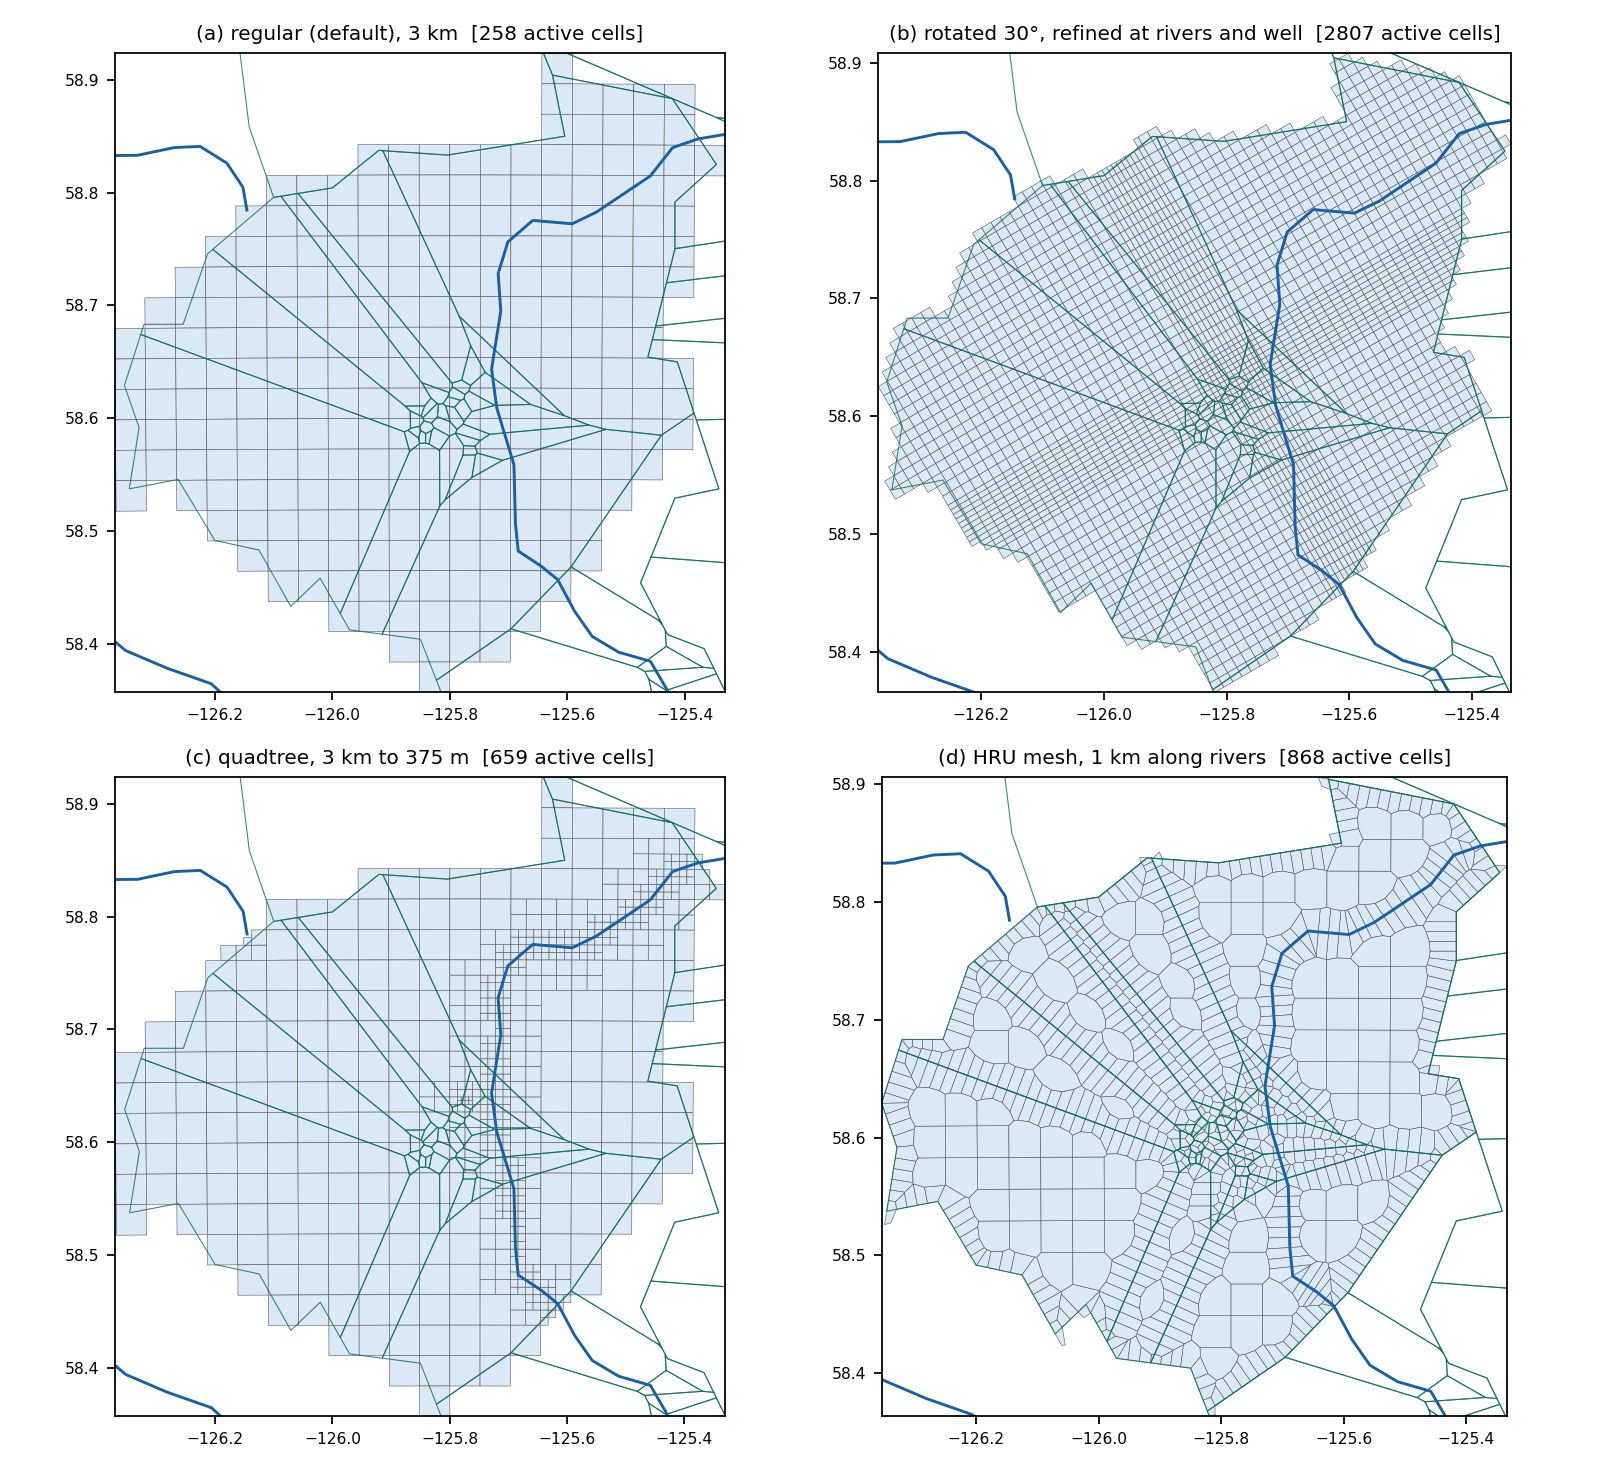
\includegraphics[width=0.78\linewidth]{figures/fig_grids.png}
\caption{The same model (Liard subbasin 52, HRU boundaries green, rivers blue) on four grids: (a) the default regular
grid; (b) rotated 30\textdegree{} and refined along rivers and around a well; (c) a quadtree refined along rivers and around the
well; (d) an HRU mesh whose cells follow HRU boundaries, with cells along the rivers.}\label{fig:grids}
\end{figure}

\subsection{Regular grids: rotation and variable spacing}
\cmd{:GridRotation} $\theta$ turns the grid $\theta$ degrees counterclockwise, for example to align columns with a valley.
The grid is built in its own rotated frame, in which every cell is still a rectangle; HRU polygons, rivers, wells and
boundaries are rotated into that frame, and MODFLOW receives the rotation as \cmd{ANGROT}. With \cmd{:GridRefinement} the grid gets variable spacing. Every base column and row that comes within the target size of a
refinement feature is divided into equal parts no larger than the target. Neighbouring columns and rows are then halved
until the widths change by at most a factor of two from one to the next. Refinement therefore always spans whole columns and rows.

\subsection{Quadtree grids}
A quadtree starts from large squares and cuts a square into four smaller ones wherever finer detail is wanted --- along a
river, say --- repeating until the cells are small enough. With \cmd{:GridType QUADTREE} a square is split into four while it is larger than the target size and a refinement feature
lies within half the target size of it. Splitting stops after \cmd{:QuadtreeMaxLevel} halvings (by default, enough to
reach the smallest target). The tree is then balanced so that neighbouring cells differ by one level at most. Where a large cell meets two
small ones its side carries the extra corner of the small cells (a hanging vertex), so MODFLOW's DISV input finds every
shared face. Because the line joining the centres of a large and a small cell is not perpendicular to their shared face,
MODFLOW's XT3D correction (the full conductance tensor) could be used. It is off by default, for two reasons found in the tests of Chapter~\ref{ch:verification}. The balanced quadtree was as
accurate without it (Thiem test). And XT3D --- even in its right-hand-side form --- slowed the Newton method badly where cells
dry and rewet: on the Liard model it took 32 instead of 7 iterations per day, and some days failed. \cmd{:FlowCorrection XT3D\_RHS} or \cmd{XT3D} switch it on.

\subsection{Meshes that follow HRU boundaries}
Picture a dot for every cell: each cell is the area closer to its own dot than to any other dot (a \emph{Voronoi} cell). If
two dots sit on opposite sides of an HRU boundary, at the same distance from it, the edge between their cells falls exactly
on that boundary. Raven places its dots this way, so the cells follow the HRU boundaries. In detail, with
\cmd{:GridType HRU\_MESH} the seed points are:
\begin{enumerate}
\item along every HRU boundary, pairs of seeds mirrored across the boundary at spacing $s_b=\min(\Delta/2,$ smallest
line refinement size (\cmd{RIVERS}, \cmd{LINES})$)$, or the \cmd{LAKES}/\cmd{POLYGONS} size where the boundary passes within
one such size of a refinement polygon, and $0.3\,s_b$ from it --- the face between the two seeds of a pair lies on the boundary;
\item seeds along refinement lines (rivers run through cell centres), in rings around refinement points (wells), and on a
staggered lattice of the target size inside and within one size around refinement polygons (lakes); seeds outside the
model's box (e.g.\ a monitoring well outside the model) are left out;
\item interior seeds on a lattice of spacing $\Delta$, kept only where no other seed is closer than about half the spacing.
\end{enumerate}
Each cell is the part of the plane closer to its seed than to any other. Raven builds it by cutting away, for each
neighbouring seed, the half of the plane that is closer to that neighbour. Each face remembers the seed on its other side, so
the connections between cells are exact. The line joining two seeds crosses their shared face at right angles, which is the
arrangement MODFLOW's standard method assumes, so no XT3D is needed. Where boundaries meet at sharp corners a cell may cover slivers of two HRUs. The overlaps are computed exactly, as for any
other grid, so the water accounts are unaffected. \cmd{GWModelSummary.txt} reports how much of each active cell's area lies
in its main HRU (typically above 99\%).

\subsection{Imported cells}
With \cmd{:GridType FILE} and \cmd{:GridFile cells.geojson ID\_FIELD} the cells are the polygons of a GeoJSON file in
longitude/latitude, one single-ring polygon per cell, numbered by the ID field (default \cmd{CELL\_ID}). Cells may be
concave, and a cell side may be shared with several smaller cells (T-junctions): neighbours are found wherever edges of two
cells lie on the same line --- within 0.1\% of the edge length, because a straight edge drawn in one map projection bends
slightly in another --- and overlap. A face made of several pieces gets their total length and their average position and
direction. Repeated vertices, which GIS exports often contain, are removed first. MODFLOW receives the grid as DISU with the
connection lengths, face widths and face directions computed from the polygons. Imported cells need not be orthogonal; for strongly non-orthogonal cells consider
\cmd{:FlowCorrection XT3D\_RHS} and check the convergence in \cmd{GWBudget.csv}.

\subsection{Connecting layers by elevation}
In a layered grid a cell connects sideways only to the cell with the same layer number. When neighbouring columns have
different profiles --- a gravel layer thinning out next to a till, say --- the same layer number can mean different
materials at different elevations. \cmd{:LayerConnection ELEVATION} writes the grid as DISU and connects every pair of
cells of neighbouring columns whose vertical intervals overlap, as staggered horizontal connections (MODFLOW's \cmd{IHC}
2), so water flows between the layers that actually touch. Pass-through cells are removed and the cells above and below
them connected directly.

\subsection{Refinement}
\begin{lstlisting}
:GridRefinement RIVERS   250                     # along :RiverGeometry lines
:GridRefinement WELLS    100                     # around pumping and monitoring wells
:GridRefinement LAKES    250                     # in and around every reservoir's lake HRU
:GridRefinement LINES    faults.geojson    200   # along any lines
:GridRefinement POLYGONS wetlands.geojson  250   # inside and around polygons
\end{lstlisting}
Sizes must be smaller than \cmd{:GridCellSize}. Refinement applies to regular (variable spacing), quadtree and HRU-mesh
grids; an imported grid is used as it is.

\cmd{LAKES} needs no extra file: the outline of the lake HRU of every Raven reservoir (\cmd{:Reservoir \dots\ :HRUID}) is taken
from \cmd{:HRUGeometry}. Fine cells around a lake place its seepage (\cmd{:ReservoirExchange}) and the exchange along its shore
more precisely. On a regular grid the rows and columns through the lake are refined; a quadtree splits the squares in and
near the lake; an HRU mesh places cells of the target size inside the lake and in a band one cell wide around it, and
shortens the spacing of its cells along the shore. \cmd{POLYGONS} works the same way for any outline in a file.

\subsection{Rivers and boundaries on any grid}
On the default grid river and boundary lines are cut into cells as before. On every other grid each piece of a line is cut exactly at the edges of the cells it crosses (rectangles along their
sides, other cells along their edges or triangle by triangle). River lengths per cell are therefore exact and do not
depend on the cell size. A stretch lying exactly on a shared cell edge
is counted once. A boundary line may be drawn along the edge of the modelled area, where the edge cells can be inactive because too little
of them is covered. Such a line is attached to the nearest active cell within one cell size, so a boundary drawn on the
watershed outline is never lost.

\subsection{Choosing a grid}
Start with the default grid and a cell size of a few kilometres. Refine where heads and exchanges change quickly: along
rivers that gain or lose much water, around pumping wells, around lakes and reservoirs that leak to the aquifer, and in
wetlands. A quadtree gives the most accuracy per cell;
an HRU mesh gives the cleanest HRU--cell linkage; a rotated regular grid is simplest when a valley has one direction. XT3D
(\cmd{:FlowCorrection XT3D\_RHS} or \cmd{XT3D}) is off by default; use it only for strongly non-orthogonal imported cells, and
check that the model still converges well.

\subsection{Grid outputs}
Every run writes \cmd{mf6/grid\_cells.geojson}: each cell as a longitude/latitude polygon with its number (as in MODFLOW and in
the hotstart file), whether it is active, its profile, its dominant HRU and its area --- ready to be joined with heads in
QGIS. For grids other than regular, \cmd{GWHeads.nc} has a \cmd{cell} dimension instead of rows and columns, and the hotstart
block is written as \cmd{:GWHeads} \emph{nlay} \cmd{1} \emph{ncells}. The grid type, cell sizes, MODFLOW format and HRU
fidelity are reported in \cmd{GWModelSummary.txt}. Setting the environment variable \cmd{RAVEN\_GW\_PROFILE=1} prints the time
taken by each stage of building the model, useful for large grids.

\section{Building the layers}\label{ch:layers}
\subsection{Land surface, model top and bedrock}
For each active column Raven needs three elevations:
\begin{description}
\item[Land surface] $z_{\mathrm{land},i}$: the average of 25 points ($5\times5$) of the DEM over the cell
(\cmd{:LandSurface}); without a DEM, the area-weighted \cmd{ELEVATION} of the HRUs in the cell.
\item[Model top] $z_{\mathrm{top},i}=z_{\mathrm{land},i}-d_{\mathrm{sz},p}$, where $d_{\mathrm{sz}}$ is the profile's
\cmd{SOIL\_ZONE\_DEPTH} (default 0, so the top is the land surface).
\item[Bedrock] $z_{\mathrm{br},i}$: the average of 25 points of the bedrock map (\cmd{:BedrockSurface}); without a map,
$z_{\mathrm{land},i}-D_p$ with $D_p$ the profile's \cmd{DEFAULT\_BEDROCK\_DEPTH}.
\end{description}
A column whose bedrock lies less than 0.5 m below its top has no room for an aquifer and is made inactive.

\subsection{Stacking the layers}
A profile lists its layers from the top down, each with a material (\emph{aquifer class}), a thickness $b_\ell$ (or
\cmd{TO\_BEDROCK}) and a type. The bottom of layer $\ell$ is
\begin{equation}
z^{(\ell)}_{\mathrm{bot},i}=
\begin{cases}
z_{\mathrm{br},i} & \text{for a \cmd{TO\_BEDROCK} layer,}\\
\max\!\left(z^{(\ell-1)}_{\mathrm{bot},i}-b_\ell,\;z_{\mathrm{br},i}\right) & \text{otherwise,}
\end{cases}
\qquad z^{(0)}_{\mathrm{bot},i}\equiv z_{\mathrm{top},i}.
\end{equation}
Layers never extend below bedrock. Two special cases:
\begin{itemize}
\item A layer (other than the first) cut to less than 0.5 m by bedrock becomes a \emph{pass-through} cell: it is given
a nominal thickness of 0.01 m and MODFLOW's \cmd{IDOMAIN}~$=-1$, which removes it from the calculation while
connecting the cells above and below it directly.
\item The model has as many layers as the thickest profile. Where a profile has fewer layers, the missing ones are
pass-through cells.
\end{itemize}

\begin{example}[: one column]
Land surface 600 m, bedrock 555 m, profile \cmd{VALLEY\_ALLUVIUM} = gravel 15 m, clay till 5 m, sand \cmd{TO\_BEDROCK}.
Top = 600 m. Layer 1 (gravel): bottom $\max(600-15,555)=585$ m. Layer 2 (till): bottom $\max(585-5,555)=580$ m.
Layer 3 (sand): bottom 555 m (to bedrock), thickness 25 m. If bedrock were at 582 m instead, layer 2 would end at
$\max(580,582)=582$ m (3 m thick), and layer 3, which runs to bedrock, would span 582 to 582 m --- zero thickness, so it becomes
a pass-through cell.
\end{example}

\begin{figure}[!htbp]\centering
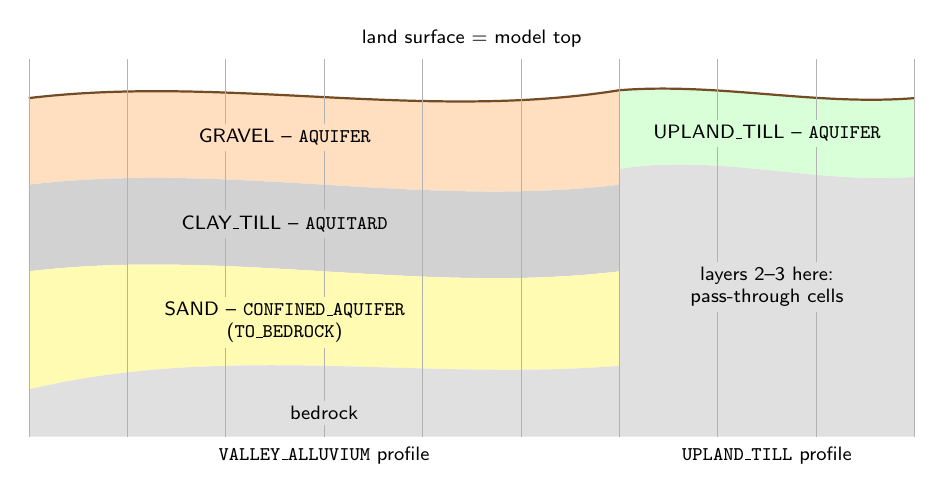
\begin{tikzpicture}[x=1.25cm,y=1.0cm,lab/.style={font=\scriptsize,align=center,inner sep=2pt}]
\fill[orange!25] (0,4.3) .. controls (2,4.6) and (4,4.0) .. (6,4.4) -- (6,3.2) .. controls (4,2.9) and (2,3.5) .. (0,3.2) -- cycle;
\fill[gray!35] (0,3.2) .. controls (2,3.5) and (4,2.9) .. (6,3.2) -- (6,2.1) .. controls (4,1.8) and (2,2.4) .. (0,2.1) -- cycle;
\fill[yellow!30] (0,2.1) .. controls (2,2.4) and (4,1.8) .. (6,2.1) -- (6,0.9) .. controls (4,0.7) and (2,1.2) .. (0,0.6) -- cycle;
\fill[black!12] (0,0.6) .. controls (2,1.2) and (4,0.7) .. (6,0.9) -- (6,0) -- (0,0) -- cycle;
\fill[green!15] (6,4.4) .. controls (7,4.5) and (8,4.2) .. (9,4.3) -- (9,3.3) .. controls (8,3.2) and (7,3.6) .. (6,3.4) -- cycle;
\fill[black!12] (6,0) -- (6,3.4) .. controls (7,3.6) and (8,3.2) .. (9,3.3) -- (9,0) -- cycle;
\draw[thick,brown!60!black] (0,4.3) .. controls (2,4.6) and (4,4.0) .. (6,4.4) .. controls (7,4.5) and (8,4.2) .. (9,4.3);
\foreach \x in {0,1,...,9} \draw[gray!60,very thin] (\x,0) -- (\x,4.8);
\node[lab,fill=white,inner sep=1pt] at (4.5,5.05) {land surface = model top};
\node[lab,fill=orange!25] at (2.6,3.8) {GRAVEL -- \cmd{AQUIFER}};
\node[lab,fill=gray!35] at (2.6,2.7) {CLAY\_TILL -- \cmd{AQUITARD}};
\node[lab,fill=yellow!30] at (2.6,1.45) {SAND -- \cmd{CONFINED\_AQUIFER}\\ (\cmd{TO\_BEDROCK})};
\node[lab,fill=black!12] at (3.0,0.3) {bedrock};
\node[lab,fill=green!15] at (7.5,3.85) {UPLAND\_TILL -- \cmd{AQUIFER}};
\node[lab,fill=black!12] at (7.5,1.9) {layers 2--3 here:\\ pass-through cells};
\node[lab,anchor=north] at (3,-0.05) {\cmd{VALLEY\_ALLUVIUM} profile};
\node[lab,anchor=north] at (7.5,-0.05) {\cmd{UPLAND\_TILL} profile};
\end{tikzpicture}
\caption{Layers are stacked from the model top and clipped at bedrock; the one-layer upland profile is padded with
pass-through cells.}\label{fig:layers}
\end{figure}

\subsection{Layer types}
\begin{table}[!htbp]\centering
\caption{Layer types.}\label{tab:types}\small
\begin{tabular}{P{0.31\linewidth}P{0.27\linewidth}P{0.348\linewidth}}\toprule\hdr
Type in the profile & MODFLOW 6 setting & What it means\\\midrule
\cmd{AQUIFER} (\cmd{UNCONFINED\_AQUIFER}) & \cmd{ICELLTYPE}=1, \cmd{ICONVERT}=1 & water table can be inside the layer: storage by $S_y$, transmissivity from the saturated thickness\\
\cmd{CONFINED\_AQUIFER} & \cmd{ICELLTYPE}=0, \cmd{ICONVERT}=0 & always full: constant transmissivity, storage by $S_s$\\
\cmd{AQUITARD}, \cmd{CONFINING\_LAYER} & as \cmd{AQUIFER}, with the low $K$ of its class & slow leaky layer, simulated explicitly\\
\cmd{AQUICLUDE} & \cmd{IDOMAIN}=0 & no flow at all through this layer (not allowed as the top layer)\\\bottomrule
\end{tabular}
\end{table}

\subsection{Material properties}
Each layer takes its properties from its aquifer class (\cmd{:AquiferClasses}): horizontal conductivity $K_h$
(\cmd{K\_HORIZ}), vertical conductivity $K_v$ (\cmd{K\_VERT}, default $K_h/10$), $S_s$ (\cmd{SPEC\_STORAGE}, default
$10^{-5}$), $S_y$ (\cmd{SPEC\_YIELD}, default 0.1) and porosity (\cmd{POROSITY}, default 0.3; stored for future transport
calculations; MODFLOW's flow calculation does not use it).

\begin{watch}
MODFLOW connects layer $\ell$ of one column sideways only to layer $\ell$ of its neighbours. Where two profiles meet,
list their layers in the same geological order, otherwise, for example, a gravel layer may connect to a clay layer.
\end{watch}

\subsection{Initial heads}
The starting head of every cell in a column is
\begin{equation}
h^0_i=\max\!\left(z_{\mathrm{land},i}-d_0,\;z_{\mathrm{low},i}+0.1\right),
\end{equation}
where $d_0$ is the profile's \cmd{INITIAL\_HEAD\_DEPTH} (or the value given by \cmd{:InitialGWHeads} in the \cmd{.rvc}
file), and $z_{\mathrm{low},i}$ is the bottom of the lowest active cell. With \cmd{:InitialGWHeads ELEVATION z}, $z$ replaces $z_{\mathrm{land},i}-d_0$ (still at least 0.1 m above the lowest active cell bottom).
A hotstart (\cmd{:GWHeads} in the \cmd{.rvc}) overrides all of this cell by cell. Optionally, a steady-state
calculation replaces these first guesses (Section~\ref{sec:init}).

\subsection{The generated MODFLOW files}
Raven writes a standard MODFLOW~6 simulation to \cmd{<output>/mf6/}: \cmd{mfsim.nam} (simulation), \cmd{sim.tdis}
(time steps), \cmd{sim.ims} (solver), \cmd{gwf.nam} (model), \cmd{gwf.dis} (grid), \cmd{gwf.npf} (conductivities and
layer types), \cmd{gwf.sto} (storage), \cmd{gwf.ic} (initial heads), \cmd{gwf.oc} (output control) and one file per
exchange package (\cmd{gwf.rch}, \cmd{gwf.drn}, \cmd{gwf.riv}, \cmd{gwf.evt}, \cmd{gwf.wel}, \cmd{gwf.ghb}, \cmd{gwf.chd},
\cmd{gwf.swx}, \cmd{gwf.res}). Grid arrays are written layer by layer, each grid row starting on a new line, which is
how MODFLOW reads them. These files can be opened in FloPy or ModelMuse; they never need editing.

\section{Parameters used to build the model}\label{sec:buildparams}
The grid and layers are built from the following parameters; the class column says where each is set, the reference column
where its default and allowed range are listed.
\begin{table}[!htbp]\centering
\caption{Parameters used to build the model.}
\begin{tabular}{>{\raggedright\arraybackslash}P{0.09\linewidth}>{\raggedright\arraybackslash}P{0.26\linewidth}>{\raggedright\arraybackslash}P{0.287\linewidth}>{\raggedright\arraybackslash}P{0.1\linewidth}>{\raggedright\arraybackslash}P{0.15\linewidth}}\toprule\hdr
Symbol & Parameter & Class (where it is set) & Units & Reference\\\midrule
$\Delta$ & \cmd{:GridCellSize} & \cmd{.rvg} option & m & Sec.~\ref{app:commands}\\
$f_{\min}$ & \cmd{:MinCellCoverage} & \cmd{.rvg} option & -- & Sec.~\ref{app:commands}\\
-- & \cmd{AQUIFER\_PROFILE} & HRU attribute (\cmd{:HRUs}, \cmd{.rvh}) & -- & Sec.~\ref{app:commands}\\
$P_k$ & HRU polygon & \cmd{:HRUGeometry} (\cmd{.rvg}) & -- & Sec.~\ref{app:commands}\\
$z_{\mathrm{land}}$ & land surface & \cmd{:LandSurface} (\cmd{.rvg}); else HRU \cmd{ELEVATION} & m & Sec.~\ref{app:commands}\\
$z_{\mathrm{br}}$ & bedrock & \cmd{:BedrockSurface} (\cmd{.rvg}); else \cmd{DEFAULT\_BEDROCK\_DEPTH} (aquifer profile) & m & Sec.~\ref{app:profile}\\
$d_{\mathrm{sz}}$ & \cmd{SOIL\_ZONE\_DEPTH} & aquifer profile & m & Sec.~\ref{app:profile}\\
$b_\ell$ & layer thickness, type & aquifer profile (\cmd{:AquiferProfiles}) & m & Sec.~\ref{app:layers}\\
$K_h$, $K_v$ & \cmd{K\_HORIZ}, \cmd{K\_VERT} & aquifer class of the layer & m/d & Sec.~\ref{app:class}\\
$S_s$, $S_y$ & \cmd{SPEC\_STORAGE}, \cmd{SPEC\_YIELD} & aquifer class of the layer & 1/m, -- & Sec.~\ref{app:class}\\
$d_0$ & \cmd{INITIAL\_HEAD\_DEPTH}; \cmd{:InitialGWHeads} & aquifer profile; \cmd{.rvc} & m & Sec.~\ref{app:profile}\\
\bottomrule
\end{tabular}
\end{table}

\section{What the generated files look like}
The model name file lists the packages Raven uses:
\begin{lstlisting}
BEGIN OPTIONS
  NEWTON
END OPTIONS
BEGIN PACKAGES
  DIS6  gwf.dis  DIS
  NPF6  gwf.npf  NPF
  STO6  gwf.sto  STO
  IC6   gwf.ic   IC
  RCH6  gwf.rch  RCH_RAVEN
  DRN6  gwf.drn  DRN_RAVEN
  RIV6  gwf.riv  RIV_RAVEN
  OC6   gwf.oc   OC
END PACKAGES
\end{lstlisting}
The grid file records the projection in its first line, so the grid can be placed on a map:
\par\noindent\begin{minipage}{\linewidth}
\begin{lstlisting}
# Lambert azimuthal equal-area projection, origin lat=58.81662353 lon=-125.4914706 (sphere R=6371007.181 m)
BEGIN DIMENSIONS
  NLAY 3
  NROW 85
  NCOL 54
END DIMENSIONS
\end{lstlisting}
\end{minipage}\par\smallskip
Boundary packages contain one line per cell with placeholder values; Raven replaces the values in memory every step, so
the files show the grid positions of recharge, drains, rivers, wells and boundaries but not their daily values.

\section{Solver settings}
Why such a small head tolerance? MODFLOW stops iterating when no head changes by more than the tolerance, but a flow is a
conductance times a head difference. The seepage drains have very large conductances (one 1 km cell with a leakance of
1~d$^{-1}$ has $10^6$~m$^2$/d), so a head tolerance of 1 cm could still leave about $10^4$~m$^3$/d of imbalance in such a cell on a
difficult day. With 0.01 mm the imbalance is a thousand times smaller than with 1 cm. The price is more Newton iterations --- in the
20-year Liard run about 10 per day on average instead of 7--8 --- and a longer run (about 15 instead of 8 minutes). The value was chosen from the
randomized tests: at 0.1 mm a few extreme set-ups (drain conductance $2\times10^7$~m$^2$/d per cell) still showed a 0.2\%
residual on single steps; at 0.01 mm none did.

\paragraph{Two-tier convergence.} A very tight tolerance can occasionally stall the Newton iterations on a hard step. The target is the tolerance above. If a step has not reached it after 100 iterations (or half the iteration limit, if that is smaller), the coupler raises
MODFLOW's own tolerance to ten times the target (0.1 mm) for the rest of that step only, and restores it for the next step. MODFLOW's own test always decides whether a step has converged. A step accepted at the relaxed tolerance is therefore as
reliable as a step of a model run with that tolerance. Only if even that fails within the iteration limit is the step
reported as not converged. \cmd{GWBudget.csv} records which
case applied (\emph{converged} = 1 target reached, 2 accepted at the relaxed tolerance, 0 not converged).
The water exchanged between Raven and MODFLOW is exact at any tolerance --- both sides use the same computed flows ---
so the tolerance only controls MODFLOW's own small numerical residual.

\begin{table}[!htbp]\centering
\caption{MODFLOW solver settings (\cmd{sim.ims}).}
\begin{tabular}{P{0.36\linewidth}P{0.14\linewidth}P{0.428\linewidth}}\toprule\hdr
IMS setting & Value & Meaning\\\midrule
\cmd{COMPLEXITY} & \cmd{COMPLEX} & robust defaults for non-linear problems\\
\cmd{OUTER\_DVCLOSE} & 0.00001 m & Newton iterations stop when no head changes by more than this (\cmd{:SolverHead\allowbreak Tolerance})\\
\cmd{OUTER\_MAXIMUM} & 500 & iteration limit (\cmd{:SolverMax\allowbreak OuterIterations})\\
\cmd{UNDER\_RELAXATION} & \cmd{DBD} & damps oscillating head changes (theta 0.7, kappa 0.07, gamma 0.1)\\
\cmd{BACKTRACKING\_NUMBER} & 20 & retries with a smaller step when the imbalance grows\\
\cmd{INNER\_MAXIMUM} & 500 & linear-solver iteration limit\\
\cmd{INNER\_DVCLOSE}, \cmd{INNER\_RCLOSE} & $0.1\times$ outer, 1 m$^3$/d & linear-solver tolerances\\
\cmd{LINEAR\_ACCELERATION} & \cmd{BICGSTAB} & linear solver\\
\cmd{PRECONDITIONER\_LEVELS} & 5 & ILU fill level\\\bottomrule
\end{tabular}
\end{table}

\section{How MODFLOW solves each time step}\label{ch:mf6}
\subsection{Time steps}
MODFLOW's time steps are generated from Raven's \cmd{:StartDate}, \cmd{:Duration} and \cmd{:TimeStep}: one transient
stress period of $N=\mathrm{round}(T/\dt)$ steps of length $\dt$, preceded by a one-day steady-state period when
\cmd{:GWInitialization STEADY\_STATE} is used. MODFLOW therefore always takes exactly one step for each Raven step.
If Raven would run more steps than MODFLOW holds, Raven stops with a clear message.

\subsection{Cells that dry and rewet: the Newton method}
An unconfined cell whose water table falls below its bottom is \emph{dry}. Older MODFLOW versions switched such cells
off, which often made the solution fail when they needed to switch back on. MODFLOW~6's Newton--Raphson method, which the coupling always uses, keeps dry cells in the calculation. The conductance
between two cells is scaled smoothly by how full the upstream cell is, and falls to zero as that cell empties. The cell
fills again naturally when water arrives. The solver settings written by Raven are:
\begin{itemize}
\item outer (Newton) iterations up to 500 (\cmd{:SolverMax\allowbreak OuterIterations}), head-change tolerance 0.00001 m (\cmd{:SolverHead\allowbreak Tolerance});
\item delta-bar-delta under-relaxation (damps oscillating head changes) and backtracking (retries a smaller change
when the residual grows);
\item inner linear solver BiCGSTAB with an ILU preconditioner of level 5, residual tolerance 1.0 m$^3$/d.
\end{itemize}
The Newton option is written without its own \cmd{UNDER\_RELAXATION} keyword, which resets a head that falls below the cell
bottom. With MODFLOW~6.6 that reset made the Newton change of a drying cell repeat unchanged at every iteration, so the
step never converged (on the Liard model this happened on most days once the thin aquitard under the gravel began to dry).
Without it, MODFLOW~6.6.3 and 6.8.1 converge in the same few iterations.
Raven runs the Newton iterations itself through MODFLOW's interface (prepare, repeated solve, finalize), so it knows
whether each step converged. If a step does not converge, MODFLOW continues (option \cmd{CONTINUE}), the step is
flagged in \cmd{GWBudget.csv}, and a safeguard limits what that step can return to Raven (Section~\ref{sec:guard}).

\subsection{Connectivity between aquifer areas}
Because dry cells carry no flow, parts of an aquifer can become disconnected when the water table falls and join
again when it rises, without any action by the user. Streams disconnect from a falling water table in the same way
(Section~\ref{ch:rivers}). To show this, \cmd{GWConnectivity.csv} reports each step:
\begin{itemize}
\item the fraction of top-layer cells of each profile that are \emph{wet}, meaning $h_i>z^{(1)}_{\mathrm{bot},i}+10^{-3}$ m;
\item the number of separate wet areas, where two wet cells belong to the same area if they share an edge
(4-neighbour connectivity; counted by a flood-fill of the wet cells).
\end{itemize}
This is a diagnostic only; it does not affect the calculation.

\subsection{Heads of dry cells}
Under the Newton method a dry cell carries no flow, and MODFLOW leaves its head at whatever value the solver reaches; it
can be far below the cell bottom (values of $-10^{8}$~m have been seen in a pumped, isolated cell). MODFLOW's own flows are
unaffected, but such a head is not a water level. Wherever the coupling needs a real water level it therefore uses the \emph{water table} of the column: the head of the
highest cell whose head is above its bottom, or the bottom of the lowest active cell if all are dry. This is used for the
reservoir's local groundwater level, in \cmd{GWHRUState.csv}, and for monitoring wells (a well screened in a dry cell
reports a missing value, \cmd{-1.2345}). The MODFLOW head file and the hotstart heads keep
MODFLOW's raw values, so a restart continues exactly.

\chapter{Coupling an existing MODFLOW 6 model}\label{ch:existing}

\begin{plain}
You give Raven your MODFLOW~6 model and tell it three things: where the model lies on the map, on what calendar date the
model's time starts, and which of the model's packages Raven should replace --- usually recharge and evaporation, which Raven
now supplies. Raven copies the model, makes the few changes shown in Figure~\ref{fig:workcopy}, and runs the copy together
with the Raven model, one day at a time. Your own files are never changed.
\end{plain}

Many users already have a calibrated MODFLOW~6 model and want to connect it to a Raven model. In this mode Raven does not
build a groundwater model. It takes the user's model as it is: the grid, the layers, the conductivities, storage, wells,
boundaries, stress periods and solver settings. Raven links its HRUs to the model's top active layer --- the highest layer
that holds water at each location --- and exchanges water there.

Only three things change, and only in a copy of the model (Figure~\ref{fig:workcopy}):
\begin{enumerate}
\item the stress periods are split into Raven time steps;
\item the packages that Raven takes over (usually recharge and evapotranspiration) are switched off;
\item two packages are added: \cmd{RCH\_RAVEN} (recharge from Raven) and \cmd{DRN\_RAVEN} (seepage back to Raven).
\end{enumerate}

\begin{figure}[!htbp]\centering% The working copy of an existing model (TikZ)
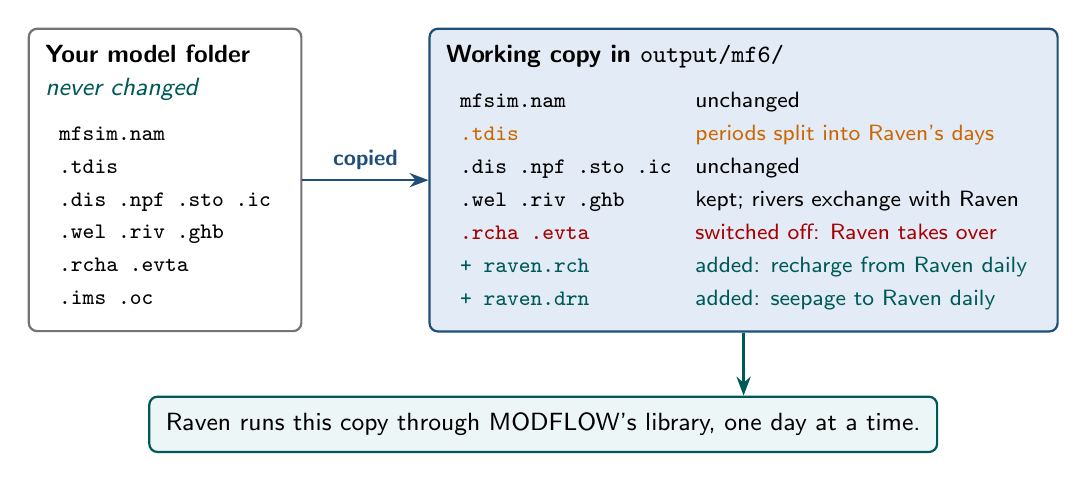
\begin{tikzpicture}[every node/.append style={execute at begin node={\hyphenpenalty=10000\exhyphenpenalty=10000}},font=\sffamily\small,arr/.style={-{Stealth[length=2.4mm]},line width=0.9pt}]
\node[draw=black!55,rounded corners=3pt,line width=0.8pt,fill=white,inner sep=6pt,align=left,anchor=north west] (L) at (0,0) {%
  \textbf{Your model folder}\\[1pt]{\itshape\color{teal!70!black}never changed}\\[5pt]
  {\footnotesize\ttfamily\begin{tabular}{l}mfsim.nam\\.tdis\\.dis .npf .sto .ic\\.wel .riv .ghb\\.rcha .evta\\.ims .oc\end{tabular}}};
\node[draw=brand,rounded corners=3pt,line width=0.8pt,fill=brandlight,inner sep=6pt,align=left,anchor=north west] (R) at ([xshift=16mm]L.north east) {%
  \textbf{Working copy in \texttt{output/mf6/}}\\[5pt]
  {\footnotesize\begin{tabular}{l@{\hspace{3mm}}l}
  \texttt{mfsim.nam} & unchanged\\
  \textcolor{orange!80!black}{\texttt{.tdis}} & \textcolor{orange!80!black}{periods split into Raven's days}\\
  \texttt{.dis .npf .sto .ic} & unchanged\\
  \texttt{.wel .riv .ghb} & kept; rivers exchange with Raven\\
  \textcolor{red!65!black}{\texttt{.rcha .evta}} & \textcolor{red!65!black}{switched off: Raven takes over}\\
  \textcolor{teal!70!black}{\texttt{+ raven.rch}} & \textcolor{teal!70!black}{added: recharge from Raven daily}\\
  \textcolor{teal!70!black}{\texttt{+ raven.drn}} & \textcolor{teal!70!black}{added: seepage to Raven daily}\\
  \end{tabular}}};
\draw[arr,brand] (L.east |- R.center) -- node[above,font=\sffamily\bfseries\footnotesize,text=brand]{copied} (R.west |- R.center);
\node[draw=teal!70!black,rounded corners=3pt,line width=0.8pt,fill=teal!7,inner sep=6pt,anchor=north] (B) at ([yshift=-8mm]current bounding box.south) {Raven runs this copy through MODFLOW's library, one day at a time.};
\draw[arr,teal!70!black] (R.south) -- (R.south |- B.north);
\end{tikzpicture}

\caption{Raven runs a working copy of the model. The copy differs from the original in three ways only; the original folder is never changed.}\label{fig:workcopy}
\end{figure}

The approach follows L.~Scantlebury's MODFLOW-USG coupling, which linked the top layer of an existing model to HRUs
through a table of overlap weights. It works for any grid, because only the top layer is linked and the model's cells are
found through MODFLOW's own memory. Regular (DIS) and polygon (DISV) grids are supported.

\section{A complete example}
\begin{lstlisting}
# Liard.rvg - Raven coupled to an existing MODFLOW 6 model
:HRUGeometry      Liard_HRUs.geojson  HRU_ID       # HRU polygons (lon/lat)
:MF6Library       /opt/mf6/libmf6.so
:MF6Simulation    model/mfsim.nam                  # the existing simulation
:MF6CRS           EPSG:32610                       # projection of the model's coordinates
:MF6StartDate     1985-10-01                       # date of the model's time zero
:RavenTakesOver   RCH_MODEL EVT_MODEL              # packages Raven replaces
:StreamPackage    RIV_STREAMS AUX SUBBASIN         # river cells linked to Raven's reaches
:SeepageToRaven   ON                               # groundwater seeping out returns to Raven
\end{lstlisting}
HRUs with an \cmd{AQUIFER\_PROFILE} in the \cmd{.rvh} file are coupled, as in the generated mode; with an existing model
the profile's layers are not used, only its seepage parameters (\cmd{SEEPAGE\_LEAKANCE}, \cmd{SEEPAGE\_SMOOTHING\_DEPTH}).
Raven's recharge must reach the \cmd{GROUNDWATER} store, exactly as in Section~\ref{sec:buildparams}.

\section{Linking HRUs to the model's cells}
Raven needs to know which grid cells lie under each HRU. MODFLOW model files do not say where on Earth the model is, so the
user supplies that information in one of three ways (give exactly one). Each coupled HRU is then linked to the top active
cell of every column it overlaps.

\paragraph{\cmd{:MF6CRS} (recommended).} The user names the model's map projection, usually as a standard EPSG code. Raven
reads the cell outlines from the model itself (column and row widths, origin and rotation for DIS grids; the cell corners for
DISV grids) and places them on the map with that projection (Figure~\ref{fig:placing}).
\begin{figure}[!htbp]\centering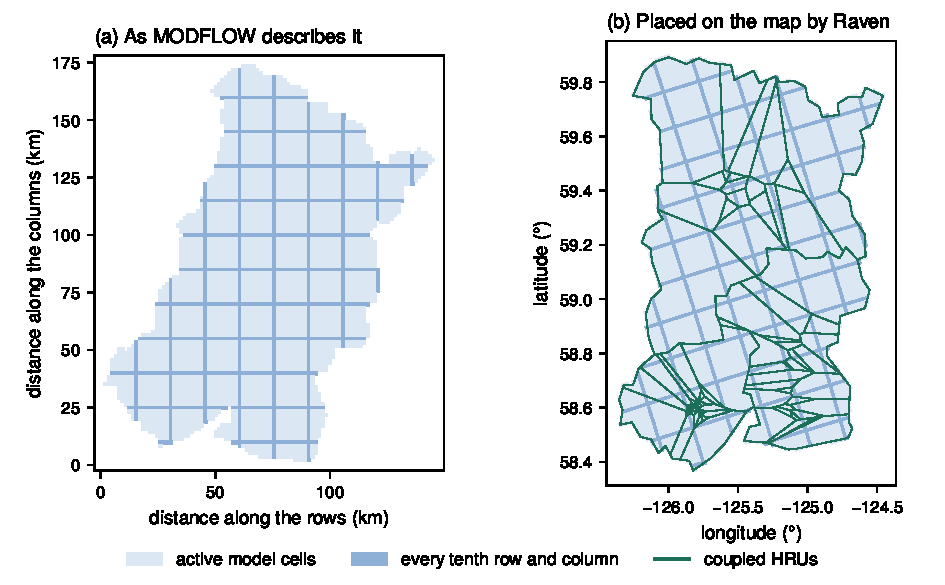
\includegraphics[width=0.95\linewidth]{figures/fig_placing.pdf}
\caption{The synthetic Liard model's cells: (a) as MODFLOW describes them, in the model's own rotated coordinates; (b) placed on the map by Raven from the projection \cmd{EPSG:32610}, under the Raven HRUs.}\label{fig:placing}
\end{figure}
 Built-in projections need no external software: Transverse Mercator (every UTM zone, north and south), Albers
equal-area and Lambert conformal conic, on the WGS84 or GRS80 (NAD83) ellipsoid. Common codes are recognised directly:
\begin{center}\small
\begin{tabularx}{\linewidth}{P{0.46\linewidth}Y}\toprule\hdr
Code & Projection\\\midrule
\cmd{EPSG:32601}--\cmd{32660}, \cmd{EPSG:32701}--\cmd{32760} & WGS84 / UTM zones, north and south\\
\cmd{EPSG:26901}--\cmd{26923} & NAD83 / UTM zones 1--23 north\\
\cmd{EPSG:3005} & NAD83 / BC Albers\\
\cmd{ESRI:102001} (or \cmd{EPSG:102001}) & Canada Albers equal-area conic (an ESRI code)\\
\cmd{EPSG:5070} & NAD83 / CONUS Albers\\
\cmd{EPSG:3978}, \cmd{EPSG:3347} & NAD83 / Canada Atlas Lambert; Statistics Canada Lambert\\\bottomrule
\end{tabularx}\end{center}
Any other projection of these three kinds is given by its parameters:
\begin{lstlisting}
:MF6CRS TMERC  lat0 lon0 k0 FE FN {WGS84|GRS80}
:MF6CRS ALBERS lat1 lat2 lat0 lon0 FE FN {WGS84|GRS80}
:MF6CRS LCC    lat1 lat2 lat0 lon0 FE FN {WGS84|GRS80}
\end{lstlisting}
The built-in formulas (Karney's series for Transverse Mercator, Snyder's for the conics) agree with the PROJ library to a few
micrometres (Section~\ref{sec:vexisting}). The small datum difference between NAD83 and WGS84 (about a metre) is ignored.

\paragraph{\cmd{:MF6GridFile}.} A GeoJSON file of the top-layer cells in longitude/latitude, numbered by an ID field
(default \cmd{CELL\_ID}) from 1 to the number of cells in a layer, as exported by GIS software. Raven checks that there is one
polygon per cell and that the polygons are the model's cells in the model's order. A map projection scales areas and turns
directions slightly, so Raven allows one common scale and one common rotation, and nothing else:
\begin{itemize}
\item every polygon's area, divided by the area MODFLOW gives the cell, must be the same for all cells within 5\%, and this
      common ratio must lie between 0.8 and 1.25 (a wrong length unit gives about 0.09 or 10.8);
\item for every pair of neighbouring cells MODFLOW connects, the two polygons must lie as far apart and in the same direction
      as MODFLOW's cells, within 20\% and 15\textdegree{} after the common scale and rotation. A shuffled numbering changes
      the distances; a mirrored one (for example rows numbered from the south: MODFLOW's row 1 is the northern row) turns
      directions around.
\end{itemize}
A file that fails either check stops the run with a message naming the first cell that does not fit.
\cmd{GWModelSummary.txt} reports the common area ratio.

\paragraph{\cmd{:OverlapWeights}.} The table of the MODFLOW-USG coupling, prepared outside Raven:
\begin{lstlisting}
:OverlapWeights
  # [HRU ID] [cell] [w = overlap area / cell area]
  2736   1204   0.35
  2736   1205   1.0
:EndOverlapWeights
\end{lstlisting}
No HRU polygons are needed. Monitoring wells cannot be located with this option.

\paragraph{No water is lost on the way.} Each HRU's recharge is shared among the cells it covers, in proportion to how much of
the HRU lies in each cell (Figure~\ref{fig:linking}a). The shares always add up to 100\%, so all the water Raven sends
arrives in MODFLOW --- even when the HRU polygons or the weights do not quite match the HRU areas in the \cmd{.rvh} file. A
mismatch changes only \emph{where} inside the HRU the water lands, not \emph{how much} (Figure~\ref{fig:linking}b). In
formula form, cell $i$ receives $V_{k\to i}=R_k\,A_k\,A_{ki}/\sum_j A_{kj}$ from HRU $k$ (Section~\ref{sec:linkage}).

\begin{figure}[!htbp]\centering% HRU over grid cells with its share in each cell (generated by make_tikz_linking.py; shares computed from the shapes)
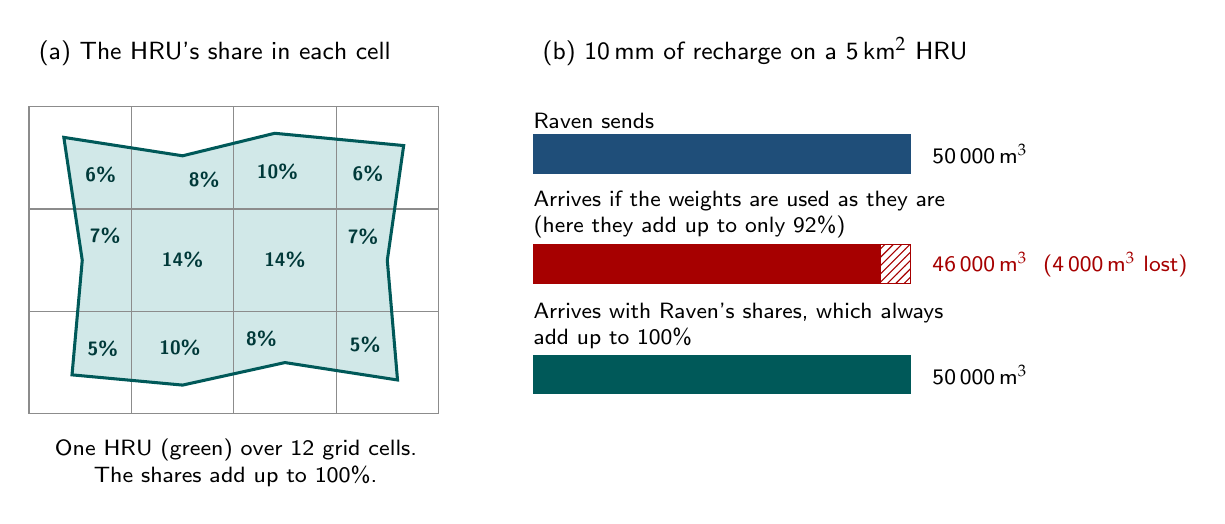
\begin{tikzpicture}[x=1mm,y=1mm,font=\sffamily\footnotesize,every node/.append style={execute at begin node={\hyphenpenalty=10000\exhyphenpenalty=10000}}]
\node[anchor=south west,font=\sffamily\small] at (0,43) {(a) The HRU's share in each cell};
\fill[teal!18] (5.46,4.94) -- (19.50,3.64) -- (32.50,6.50) -- (46.80,4.29) -- (45.50,19.50) -- (47.58,34.06) -- (31.20,35.62) -- (19.50,32.76) -- (4.42,35.10) -- (6.76,19.50) -- cycle;
\draw[black!45,line width=0.4pt] (0,0) rectangle (13,13);
\draw[black!45,line width=0.4pt] (0,13) rectangle (13,26);
\draw[black!45,line width=0.4pt] (0,26) rectangle (13,39);
\draw[black!45,line width=0.4pt] (13,0) rectangle (26,13);
\draw[black!45,line width=0.4pt] (13,13) rectangle (26,26);
\draw[black!45,line width=0.4pt] (13,26) rectangle (26,39);
\draw[black!45,line width=0.4pt] (26,0) rectangle (39,13);
\draw[black!45,line width=0.4pt] (26,13) rectangle (39,26);
\draw[black!45,line width=0.4pt] (26,26) rectangle (39,39);
\draw[black!45,line width=0.4pt] (39,0) rectangle (52,13);
\draw[black!45,line width=0.4pt] (39,13) rectangle (52,26);
\draw[black!45,line width=0.4pt] (39,26) rectangle (52,39);
\draw[teal!70!black,line width=1.1pt] (5.46,4.94) -- (19.50,3.64) -- (32.50,6.50) -- (46.80,4.29) -- (45.50,19.50) -- (47.58,34.06) -- (31.20,35.62) -- (19.50,32.76) -- (4.42,35.10) -- (6.76,19.50) -- cycle;
\node[font=\sffamily\bfseries\scriptsize,text=teal!45!black,inner sep=0.5pt] at (9.37,8.21) {5\%};
\node[font=\sffamily\bfseries\scriptsize,text=teal!45!black,inner sep=0.5pt] at (9.67,22.57) {7\%};
\node[font=\sffamily\bfseries\scriptsize,text=teal!45!black,inner sep=0.5pt] at (9.10,30.37) {6\%};
\node[font=\sffamily\bfseries\scriptsize,text=teal!45!black,inner sep=0.5pt] at (19.17,8.35) {10\%};
\node[font=\sffamily\bfseries\scriptsize,text=teal!45!black,inner sep=0.5pt] at (19.50,19.50) {14\%};
\node[font=\sffamily\bfseries\scriptsize,text=teal!45!black,inner sep=0.5pt] at (22.24,29.67) {8\%};
\node[font=\sffamily\bfseries\scriptsize,text=teal!45!black,inner sep=0.5pt] at (29.53,9.47) {8\%};
\node[font=\sffamily\bfseries\scriptsize,text=teal!45!black,inner sep=0.5pt] at (32.50,19.50) {14\%};
\node[font=\sffamily\bfseries\scriptsize,text=teal!45!black,inner sep=0.5pt] at (31.56,30.78) {10\%};
\node[font=\sffamily\bfseries\scriptsize,text=teal!45!black,inner sep=0.5pt] at (42.70,8.71) {5\%};
\node[font=\sffamily\bfseries\scriptsize,text=teal!45!black,inner sep=0.5pt] at (42.43,22.47) {7\%};
\node[font=\sffamily\bfseries\scriptsize,text=teal!45!black,inner sep=0.5pt] at (43.05,30.47) {6\%};
\node[anchor=north,align=center,text width=50mm] at (26,-2) {One HRU (green) over 12 grid cells.\\The shares add up to 100\%.};
\node[anchor=south west,font=\sffamily\small] at (64,43) {(b) 10\,mm of recharge on a 5\,km$^2$ HRU};
\node[anchor=south west,align=left,inner sep=0pt] at (64,36.2) {Raven sends};
\fill[brand] (64,30.5) rectangle (112,35.5);
\node[anchor=west] at (113.5,33) {50\,000\,m$^3$};
\node[anchor=south west,align=left,inner sep=0pt] at (64,22.2) {Arrives if the weights are used as they are\\(here they add up to only 92\%)};
\fill[red!65!black] (64,16.5) rectangle (108.16,21.5);
\draw[red!65!black,pattern=north east lines,pattern color=red!65!black] (108.16,16.5) rectangle (112,21.5);
\node[anchor=west,text=red!65!black] at (113.5,19) {46\,000\,m$^3$ \ (4\,000\,m$^3$ lost)};
\node[anchor=south west,align=left,inner sep=0pt] at (64,8.2) {Arrives with Raven's shares, which always\\add up to 100\%};
\fill[teal!70!black] (64,2.5) rectangle (112,7.5);
\node[anchor=west] at (113.5,5) {50\,000\,m$^3$};
\end{tikzpicture}

\caption{Sharing an HRU's water among cells. (a) The HRU's share in each cell, computed from the shapes; the shares add up to 100\%. (b) Weights that add up to only 92\% would lose 8\% of the water; Raven's shares always add up to 100\%, so every cubic metre arrives.}\label{fig:linking}
\end{figure}

In the older MODFLOW-USG coupling the weights were used as given, so the recharge volume depended on how carefully the HRUs
were drawn. Rates passed to MODFLOW use MODFLOW's own cell areas. \cmd{GWModelSummary.txt} reports how much of the coupled
HRUs' area lies on active cells; a low value usually means a wrong projection or HRUs outside the model.

\section{Time}\label{sec:existingtime}
MODFLOW models divide time into \emph{stress periods}: stretches of time, often a month, during which inputs such as pumping
rates stay the same. Raven works in days. Raven keeps the model's stress periods and their dates, and splits each period into
Raven days (Figure~\ref{fig:periods}), so the model's own changes --- a well pumping harder in summer, a boundary level
changing --- still happen on their dates.

\cmd{:MF6StartDate} is the calendar date on which the model's time starts. Each stress period must contain a whole number of
Raven time steps, and Raven's run may not go past the end of the model; otherwise the run stops with a message. Steady-state
periods (solved as the long-term balance) stay steady-state.

\paragraph{Steady-state models.} Many calibrated models are steady state: no storage package (or one that marks every period
steady) and a single stress period whose length has no meaning (often one second or one day). Raven stretches that period
over its run, so every Raven step is a steady-state solution with that step's recharge: the aquifer responds at once, without
storage. \cmd{GWModelSummary.txt} says so, and the storage column of \cmd{GWBudget.csv} stays zero (the balance residual is
reported as MODFLOW's error). Because such a model has no time of its own, Raven may start on any date from
\cmd{:MF6StartDate} on.

\begin{figure}[!htbp]\centering% Stress periods, Raven's days and a restart after 40 days (TikZ; 1 mm per day)
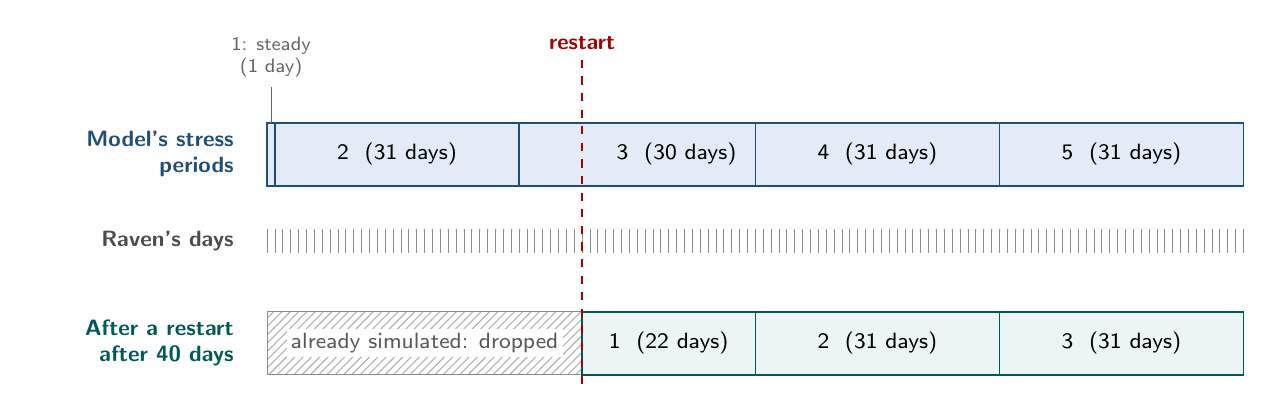
\begin{tikzpicture}[every node/.append style={execute at begin node={\hyphenpenalty=10000\exhyphenpenalty=10000}},x=1mm,y=1mm,font=\sffamily\footnotesize,
  rowlab/.style={anchor=east,align=right,text width=25mm,font=\sffamily\footnotesize\bfseries},
  per/.style={draw=brand,fill=brandlight,line width=0.6pt},
  new/.style={draw=teal!70!black,fill=teal!8,line width=0.6pt}]
% row 1: the model's stress periods (1 steady day, then 31, 30, 31, 31 days)
\node[rowlab,text=brand] at (-3,0) {Model's stress\\periods};
\draw[per] (0,-4) rectangle (1,4);
\foreach \a/\b/\t/\lx in {1/32/{2 \ (31 days)}/16.5, 32/62/{3 \ (30 days)}/52, 62/93/{4 \ (31 days)}/77.5, 93/124/{5 \ (31 days)}/108.5}{
  \draw[per] (\a,-4) rectangle (\b,4); \node at (\lx,0) {\t};}
\draw[black!60] (0.5,4) -- (0.5,8.5) node[above,align=center,font=\sffamily\scriptsize] {1: steady\\(1 day)};
% row 2: Raven's days
\node[rowlab,text=black!70] at (-3,-11) {Raven's days};
\foreach \d in {0,...,124}{\draw[black!45,line width=0.3pt] (\d,-12.5) -- (\d,-9.5);}
% row 3: after a restart after 40 days
\node[rowlab,text=teal!70!black] at (-3,-24) {After a restart\\after 40 days};
\draw[black!45,fill=black!6,pattern=north east lines,pattern color=black!30] (0,-28) rectangle (40,-20);
\node[fill=white,inner sep=1.5pt,text=black!65] at (20,-24) {already simulated: dropped};
\foreach \a/\b/\t in {40/62/{1 \ (22 days)}, 62/93/{2 \ (31 days)}, 93/124/{3 \ (31 days)}}{
  \draw[new] (\a,-28) rectangle (\b,-20); \node at ({(\a+\b)/2},-24) {\t};}
% the restart
\draw[red!65!black,dashed,line width=0.9pt] (40,12) -- (40,-30);
\node[above,text=red!65!black,font=\sffamily\bfseries\footnotesize] at (40,12) {restart};
\end{tikzpicture}

\caption{Top: a model with a one-day steady period followed by periods of 31, 30, 31 and 31 days, and Raven's days. Bottom: after a restart 40 days into the model, the time already simulated is dropped, period~3 keeps its last 22 days, and the periods are renumbered; each keeps its own well rates and boundary levels.}\label{fig:periods}
\end{figure}

\paragraph{Starting later: restarts.} Raven may start later than the model's time zero --- when a run is continued from
\cmd{solution.rvc}, or begins part-way through the model. Raven then removes the stress periods already simulated from the
working copy, shortens the period that holds Raven's start, and renumbers the periods of every package; the new first period
takes the inputs that were in force on Raven's start date (Figure~\ref{fig:periods}, bottom). This is safe for packages whose period
entries replace one another (WEL, RIV, GHB, CHD, DRN, list-based RCH and EVT, STO, OC, the water mover MVR), and for
array-based recharge and ET and the advanced packages (SFR, LAK, MAW, UZF) when at most one period entry comes before Raven's
start. Such a package with several earlier entries, whose settings build on one another, stops such a run, as do time-varying conductivity or storage
(\cmd{TVK6}, \cmd{TVS6}) and a simulation holding more than one model (only the coupled model's periods would be
renumbered); Raven must then start at \cmd{:MF6StartDate}. A package that uses time series stops any later start, even one
inside the first period, because the times of a series count from the model's own start. A time of day in Raven's
\cmd{:StartDate} counts in the offset, and the working copy's \cmd{START\_DATE\_TIME} is set to Raven's start.

\section{Units}
Length units (metres, feet, centimetres) are read from the discretization package and time units (seconds to years) from
the time discretization. Heads, flows, rates, conductances and coordinates are converted at the interface; Raven's outputs
are always in metres and days.

\section{Packages}
\begin{table}[!htbp]\centering
\caption{How the model's packages are treated.}\label{tab:extpkgs}
\begin{tabularx}{\linewidth}{P{0.30\linewidth}Y}\toprule\hdr
Package & Treatment\\\midrule
Recharge, evapotranspiration, UZF & must be named in \cmd{:RavenTakesOver} (removed; Raven supplies recharge) or in \cmd{:KeepPackages} (they stay). An undeclared one stops the run, so recharge is never counted twice\\
Stream package (\cmd{:StreamPackage}) & a RIV, DRN or GHB package whose flows go to Raven's reaches: to the subbasin in an auxiliary variable (\cmd{AUX} name, default \cmd{SUBBASIN}), or to the subbasin of the dominant HRU of the cell (\cmd{DOMINANT\_HRU}). Losing reaches take the water from the channel; a loss that cannot be supplied is carried to the next step\\
\cmd{DRN\_RAVEN} (\cmd{:SeepageToRaven ON}) & added at the top of the top active cell of coupled columns; the discharge returns to Raven (Section~\ref{ch:seepage})\\
\cmd{RCH\_RAVEN} & added at the top active cell of every coupled column. MODFLOW ignores recharge on specified-head cells, so columns whose top cell is specified-head (read from the model each step, as the stress periods may change them) take none: each HRU's recharge is spread over its other cells, and recharge of an HRU lying only on such cells is reported in \cmd{GWBudget.csv} (\emph{recharge onto CHD cells})\\
Water mover (MVR) & kept; movers from or to a package Raven takes over are removed from the working copy (MODFLOW would stop on a package that is no longer there), and \cmd{GWModelSummary.txt} reports how many. A stream package that sends water through the mover is refused, because Raven would take the same water from the aquifer a second time\\
All other packages & kept unchanged: wells, head boundaries, drains, lakes, streamflow routing and so on. Their simulated flows, including the water they pass to the mover, enter the balance check (\cmd{GWBudget.csv}, column \emph{other model packages})\\\bottomrule
\end{tabularx}
\end{table}

\section{Safeguards}
Every one of these stops the run with a message that names the problem and the fix:
\begin{itemize}
\item a recharge, ET or UZF package not declared taken over or kept; \cmd{:RavenTakesOver} naming another kind of package;
      a stream package that is not RIV, DRN or GHB, or one that sends water through the mover; a package name not in the
      model name file; a mover whose period data sit in another file, when it names a package Raven takes over;
\item several groundwater models in the simulation and no \cmd{:MF6Model};
\item a Raven start before the model's time zero (\cmd{:MF6StartDate}); a later start that the model's packages cannot follow (Section~\ref{sec:existingtime}); a stress period that is not a whole number of Raven steps; a Raven run longer than
      the model;
\item a cell file whose polygons are not the model's cells (count, numbering or area);
\item a stream cell whose subbasin does not exist or is disabled;
\item options of the generated mode left in the \cmd{.rvg} file (grid options, \cmd{:GridCellSize}, \cmd{:LandSurface},
      \cmd{:BedrockSurface}, the solver settings, \cmd{:Wells}, head boundaries, \cmd{:RiverGeometry}, \cmd{:GWInitialization}),
      or none or several ways of linking HRUs;
\item a simulation with more than one solution (for example a transport model with its own IMS): Raven drives one
      groundwater-flow solution;
\item adaptive time stepping (\cmd{ATS6} in the TDIS options): Raven needs fixed time steps;
\item a Raven calendar other than Gregorian (the dates of the two models are compared day by day);
\item \cmd{:WriteNetCDFHeads} with \cmd{:OverlapWeights} (a weight table has no coordinates);
\item a simulation that lies inside Raven's own working folder (\cmd{output/mf6/}), which Raven overwrites.
\end{itemize}
A solver tolerance looser than 0.01 m is reported in \cmd{GWModelSummary.txt}.

\section{The model's solver}
The model's own solver settings (\cmd{.ims}) are used. On a step that needs more than 100 outer iterations (or half the
model's iteration limit, if that is smaller) the coupler relaxes
MODFLOW's head tolerance tenfold for the rest of that step (as for generated models, Section~\ref{ch:mf6}), in the model's
units. The first coupled step is often the hardest --- a steady-state period solved from the model's starting heads with
Raven's recharge --- so allow at least 500 outer iterations (\cmd{OUTER\_MAXIMUM}). A step that does not converge is flagged
in \cmd{GWBudget.csv} and the exchange on it is limited, as described in Section~\ref{ch:mf6}. For this, the working copy's
\cmd{mfsim.nam} always has the \cmd{CONTINUE} option: without it, MODFLOW would stop the whole simulation at the first step
that does not converge.

With MODFLOW versions before 6.8, the \cmd{UNDER\_RELAXATION} keyword of the model's \cmd{NEWTON} option can make a step in
which a cell dries repeat the same Newton change at every iteration and never converge (the synthetic Liard model failed on
every day with MODFLOW~6.6.3 and converged on every day with 6.8.1). Raven reads the library's version, writes it
to \cmd{GWModelSummary.txt}, and warns when an older version meets that keyword: use MODFLOW~6.8 or newer, or remove the
keyword from the model's name file (on the synthetic model the results with 6.8.1 are identical either way).

\section{Outputs and restarts}
All outputs of Chapter~\ref{ch:c6} are written. Raven copies the whole folder that holds the simulation file (the simulation
may read files from anywhere in it), so keep the model in a folder of its own; old results (\cmd{.hds}, \cmd{.cbc},
\cmd{.lst}, \cmd{.grb}, \cmd{.bud}, \cmd{.cbb}) are not copied. The simulation file may have any name: the working copy
always holds it as \cmd{mfsim.nam}, the name MODFLOW's library opens. In \cmd{GWHRUState.csv} the water-table depth is
measured from the top of the model's top active cell, which with an existing model stands for the land surface. \cmd{mf6/} holds the working copy of the simulation, with Raven's packages
(\cmd{raven.rch}, \cmd{raven.drn}); \cmd{mf6/grid\_cells.geojson} shows the linked cells (not with \cmd{:OverlapWeights}).
Restarts store the heads in the model's layout (\cmd{:GWHeads} \emph{nlay nrow ncol} for DIS, \emph{nlay} \cmd{1} \emph{ncells}
for DISV); on a restart Raven writes them as the initial heads of the working copy (\cmd{raven.ic}) and renumbers the stress
periods as described above. A restarted run reproduces a continuous one (Section~\ref{sec:vexisting}).

\section{Worked example}
\cmd{examples/Liard\_existing\_model/} holds a MODFLOW 6 model of the Liard coupled area built independently of Raven: a
regular grid of 1.5 km cells rotated 15\textdegree{} in UTM zone 10N, four layers with spatially varying conductivity,
a one-day steady-state period followed by 24 monthly periods, two wells with seasonal pumping, 239 river cells carrying
their subbasin ID in an auxiliary variable, a head boundary at the outlet, and its own recharge and ET packages. The \cmd{.rvg}
file of Section~\ref{ch:existing} couples it to the Liard Raven model; the two-year run takes about four minutes.

\section{Checking the calibration}
Replacing a calibrated recharge package with Raven's recharge changes the model's water budget. Compare the coupled heads and
budget with a run of the original model before using the results: large differences mean Raven's recharge, or the
recharge the model was calibrated with, needs attention.

\section{Current limits}
DISU models, water-table ET from Raven (the model's own ET package can be kept), surface-store and reservoir exchanges, and
the conductance limit of generated river cells are not available in this mode; the stream package's stage comes from the
model. Restarts after the model's time zero need daily or longer Raven time steps.

\chapter{Water exchanges between Raven and MODFLOW}\label{ch:c4}
Raven and MODFLOW exchange water in eight ways (Table~\ref{tab:exchanges}). Each section below explains what the exchange represents and gives its equations. It then says what Raven does with the
result, which safeguards keep the water accounts exact, which inputs control it, where to see it in the outputs, and gives
a worked example.

\begin{plain}
Water crosses between the two models in eight places. The two main ones are \emph{recharge} --- water soaking down from
Raven's soil to the water table --- and \emph{seepage} --- groundwater coming back up where the water table reaches the ground.
Rivers, lakes and reservoirs, wetlands, wells and evaporation from a shallow water table make up the rest. For each one this
chapter gives the formula, a worked example with numbers, and the checks that make sure no water is created or lost on the
way.
\end{plain}
\begin{table}[!htbp]\centering
\caption{The eight exchanges between Raven and MODFLOW.}\label{tab:exchanges}\small
\begin{tabular}{lllll}\toprule\hdr
Exchange & Direction & MODFLOW package & Raven side & Section\\\midrule
Recharge & Raven $\to$ aquifer & RCH & \cmd{GROUNDWATER} & \ref{ch:recharge}\\
Seepage & aquifer $\to$ Raven & DRN & lowest soil layer & \ref{ch:seepage}\\
Rivers & both & RIV & reach inflow & \ref{ch:rivers}\\
Water-table ET & aquifer $\to$ air & EVT & unmet PET & \ref{ch:et}\\
Wetlands, lakes & both & RIV & HRU store & \ref{ch:stores}\\
Reservoirs & both & WEL & reservoir seepage & \ref{ch:reservoirs}\\
Wells & out (or in) & WEL & time series & \ref{ch:wells}\\
Boundaries & both & GHB, CHD & time series & \ref{ch:wells}\\\bottomrule
\end{tabular}\end{table}
\begin{figure}[!htbp]\centering
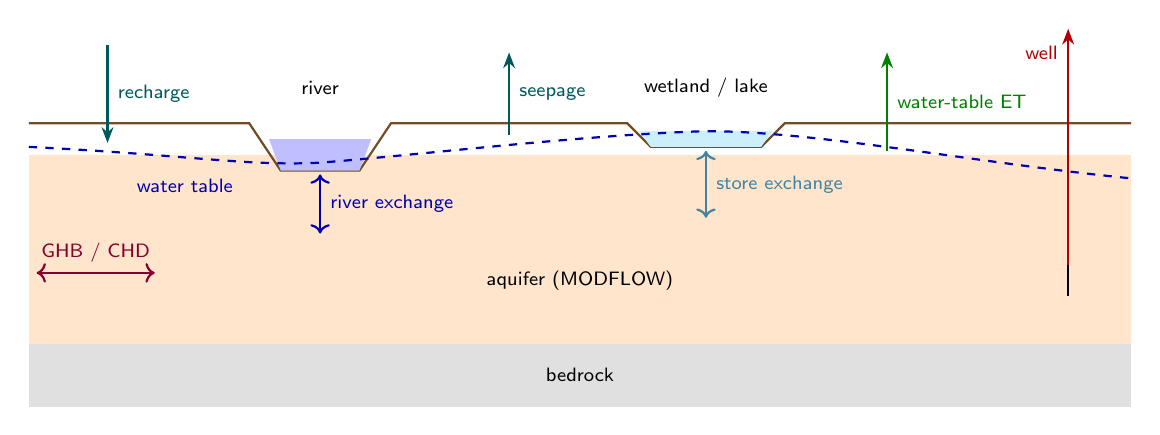
\begin{tikzpicture}[x=1cm,y=1cm,lab/.style={font=\scriptsize,align=center},ar/.style={-{Stealth[length=2mm]},thick}]
\fill[orange!20] (0,0.8) rectangle (14,3.2); \fill[black!12] (0,0) rectangle (14,0.8);
\draw[thick,brown!60!black] (0,3.6) -- (2.8,3.6) -- (3.2,3.0) -- (4.2,3.0) -- (4.6,3.6) -- (7.6,3.6) -- (7.9,3.3) -- (9.3,3.3) -- (9.6,3.6) -- (14,3.6);
\fill[blue!25] (3.05,3.4) -- (4.35,3.4) -- (4.2,3.0) -- (3.2,3.0) -- cycle; \node[lab] at (3.7,4.05) {river};
\fill[cyan!20] (7.75,3.5) -- (9.45,3.5) -- (9.3,3.3) -- (7.9,3.3) -- cycle; \node[lab] at (8.6,4.05) {wetland / lake};
\draw[dashed,blue!70!black,thick] (0,3.3) .. controls (2,3.2) and (2.8,3.05) .. (3.7,3.1) .. controls (5,3.2) and (7,3.45) .. (8.6,3.5) .. controls (10,3.5) and (12,3.1) .. (14,2.9);
\node[lab,blue!70!black,anchor=west] at (1.25,2.8) {water table};
\draw[ar,teal!70!black] (1.0,4.6) -- node[lab,right]{recharge} (1.0,3.35);
\draw[ar,teal!70!black] (6.1,3.45) -- node[lab,right]{seepage} (6.1,4.5);
\draw[ar,blue!70!black,<->] (3.7,2.95) -- node[lab,right]{river exchange} (3.7,2.2);
\draw[ar,cyan!60!black,<->] (8.6,3.25) -- node[lab,right]{store exchange} (8.6,2.4);
\draw[ar,green!50!black] (10.9,3.25) -- node[lab,right]{water-table ET} (10.9,4.5);
\draw[thick] (13.2,4.7) -- (13.2,1.4); \draw[ar,red!70!black] (13.2,1.8) -- node[lab,left,pos=0.9]{well} (13.2,4.8);
\draw[ar,purple!70!black,<->] (0.1,1.7) -- node[lab,above]{GHB / CHD} (1.6,1.7);
\node[lab] at (7,1.6) {aquifer (MODFLOW)}; \node[lab] at (7,0.4) {bedrock};
\end{tikzpicture}
\caption{The exchanges between Raven (above the water table) and MODFLOW (below). Reservoir seepage works like the store
exchange, through Raven's reservoir seepage law.}\label{fig:allexch}
\end{figure}

\section{Recharge: from Raven to the water table}\label{ch:recharge}
\subsection{Where recharge comes from}
Any Raven process that moves water into \cmd{GROUNDWATER} in a coupled HRU produces recharge --- no special process is
needed. For example, in the Liard model the percolation from the fast reservoir is sent to \cmd{GROUNDWATER} for coupled
HRUs:
\par\noindent\begin{minipage}{\linewidth}
\begin{lstlisting}
:Percolation PERC_CONSTANT FAST_RESERVOIR GROUNDWATER
  :-->Conditional HRU_GROUP IS AquiferHRUs
\end{lstlisting}
\end{minipage}\par\smallskip
At the end of a day, the \cmd{GROUNDWATER} store of HRU $k$ holds $r_k$ mm; this is the recharge of that day. Raven
counts it as water leaving Raven (its balance, Section~\ref{ch:balance}), and it is empty again at the start of the
next day.

\subsection{Volume of recharge}
\begin{equation}
V_k=\frac{r_k}{1000}\,A_k \quad[\mathrm{m}^3],
\end{equation}
with $A_k$ the HRU area from the \cmd{.rvh} file in m$^2$.

\subsection{Optional recharge delay}
Where the water table is deep, water takes time to cross the unsaturated zone. With the aquifer profile parameter \cmd{RECHARGE\_DELAY}~$\tau>0$ (Section~\ref{app:profile})
(days) the recharge passes through a linear reservoir $S_k$ before reaching the water table:
\begin{equation}
S_k^{*}=S_k^{n}+V_k,\qquad V_k^{\mathrm{out}}=S_k^{*}\left(1-e^{-\dt/\tau}\right),\qquad S_k^{n+1}=S_k^{*}-V_k^{\mathrm{out}} .
\end{equation}
With $\tau=0$ the delay is off and $V_k^{\mathrm{out}}=V_k$. The delay store is reported in \cmd{GWBudget.csv}, saved in
\cmd{solution.rvc} (\cmd{:GWRechargeStore}) and read back on hotstart.
\begin{example}[: recharge delay]
$\tau=60$ d, $\dt=1$ d: each day $1-e^{-1/60}=1.65\%$ of the store is released. A single 1\,000 m$^3$ pulse reaches the
water table as 16.5 m$^3$ on the first day, then less each day; after 60 days 63\% of it has arrived
(Figure~\ref{fig:curves}a).
\end{example}

\subsection{Spreading recharge over the cells}
The released volume is shared among the HRU's cells in proportion to overlap. Cells whose top cell holds a fixed head
(Section~\ref{ch:wells}) are skipped, because MODFLOW ignores recharge there:
\begin{equation}
Q^{\mathrm{rch}}_i=\sum_{k\in\mathcal{K}}\frac{V_k^{\mathrm{out}}}{\dt}\,\frac{A_{k,i}}{\sum_{j\notin\mathcal{C}}A_{k,j}}
\quad[\mathrm{m}^3/\mathrm{d}],\qquad R_i=\frac{Q^{\mathrm{rch}}_i}{\Delta^2}\quad[\mathrm{m/d}],
\end{equation}
where $\mathcal{C}$ are the fixed-head columns. $R_i$ is the recharge rate given to MODFLOW's RCH package, applied to the top cell of the column
(the top layer of an active column is always active). The fractions for one HRU always add up to one, so exactly $V_k^{\mathrm{out}}$
enters MODFLOW. If an HRU lies entirely on fixed-head cells, its recharge passes to that boundary and is reported in the
column \emph{recharge onto CHD cells}.
\begin{example}[: spreading recharge]
The 10 km$^2$ HRU of the Section~\ref{ch:grid} example receives 2 mm in a day: $V=0.002\times10^7=20\,000$ m$^3$. The three
cells get 8\,000, 7\,000 and 5\,000 m$^3$/d; for 4 km$^2$ cells the recharge rates are 2.0, 1.75 and 1.25 mm/d
(plus any recharge from other HRUs in the same cells).
\end{example}

\begin{figure}[!htbp]\centering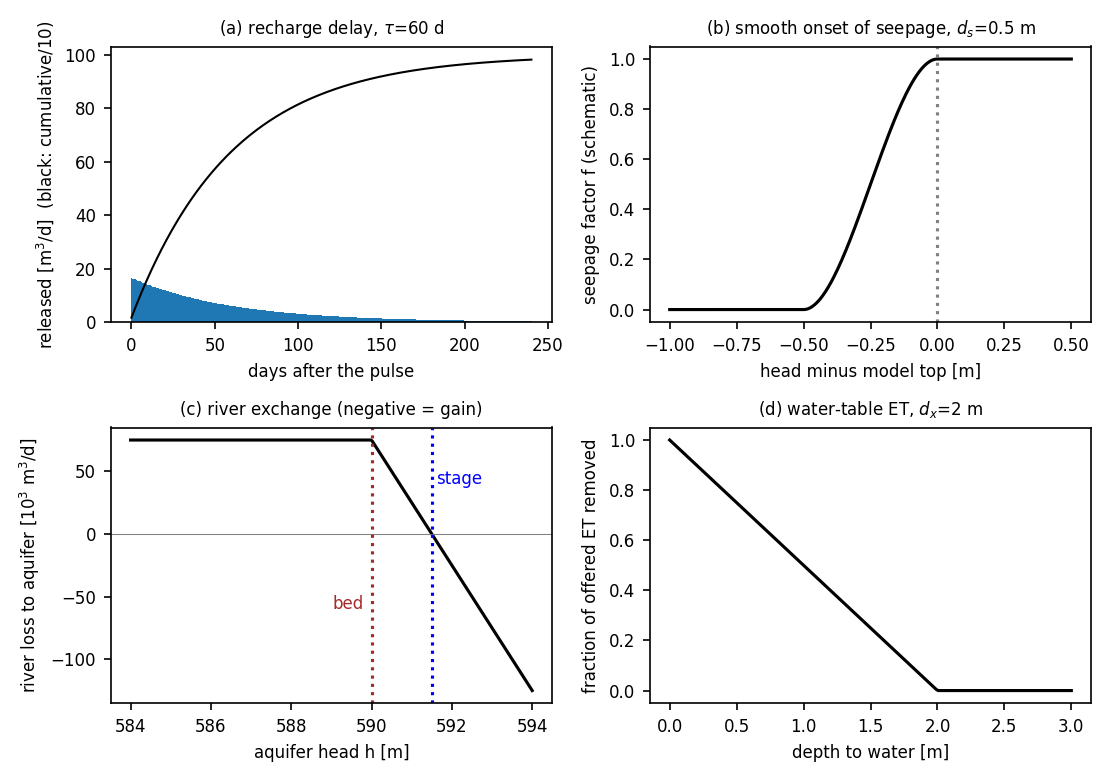
\includegraphics[width=\linewidth]{figures/fig_curves.png}
\caption{Response curves of four exchanges: (a) recharge delay reservoir after a 1\,000 m$^3$ pulse ($\tau=60$ d);
(b) seepage factor near the model top ($d_s=0.5$ m); (c) river flow against aquifer head; (d) water-table ET against
depth ($d_x=2$ m).}\label{fig:curves}\end{figure}

\begin{refcard}{recharge}
\textbf{Sources/sinks.} Moves water from \cmd{GROUNDWATER} of each coupled HRU to the aquifer (MODFLOW RCH package \cmd{RCH\_RAVEN}, top cell of each
active column), optionally through the recharge-delay store (internal to the coupling, saved in \cmd{solution.rvc}).\par\smallskip
\textbf{Constraints/notes.} In a coupled HRU \cmd{GROUNDWATER} is a pass-through: no Raven process may draw water from it (start-up error). Recharge is
never negative. The volume of each HRU is conserved exactly; recharge of HRUs lying wholly on fixed-head cells is reported
separately.\par\smallskip
\par\noindent\begin{minipage}{\linewidth}\textbf{Command syntax}
\begin{lstlisting}
# .rvi -- any process that moves water into GROUNDWATER in coupled HRUs, e.g.
:Percolation  PERC_CONSTANT  FAST_RESERVOIR  GROUNDWATER
  :-->Conditional HRU_GROUP IS AquiferHRUs
# .rvp -- optional recharge delay, per aquifer profile
:AquiferProfileParameters
  :Attributes,     RECHARGE_DELAY
  :Units,          d
  VALLEY_ALLUVIUM, 30.0
:EndAquiferProfileParameters
\end{lstlisting}
\end{minipage}\par\smallskip
\par\noindent\begin{minipage}{\linewidth}\textbf{Parameters}\par\smallskip
\begin{tabular}{>{\raggedright\arraybackslash}P{0.09\linewidth}>{\raggedright\arraybackslash}P{0.26\linewidth}>{\raggedright\arraybackslash}P{0.283\linewidth}>{\raggedright\arraybackslash}P{0.1\linewidth}>{\raggedright\arraybackslash}P{0.15\linewidth}}\toprule\hdr \hdr Symbol & Parameter & Class (where it is set) & Units & Reference\\\midrule
$r_k$ & \cmd{GROUNDWATER} & Raven state variable of HRU $k$ (filled by the chosen process) & mm & Raven state var.\\
$A_k$ & \cmd{AREA} & HRU (\cmd{:HRUs}, \cmd{.rvh}) & km$^2$ & Raven manual\\
$\tau$ & \cmd{RECHARGE\_DELAY} & aquifer profile (\cmd{:AquiferProfile\allowbreak Parameters}) & d & Sec.~\ref{app:profile}\\
$A_{k,i}$ & overlap area & computed from \cmd{:HRUGeometry} (\cmd{.rvg}) & m$^2$ & Sec.~\ref{ch:grid}\\
$\Delta$ & \cmd{:GridCellSize} & \cmd{.rvg} option & m & Sec.~\ref{app:commands}\\
\bottomrule\end{tabular}\end{minipage}\par\smallskip
\textbf{Outputs.} \cmd{GWBudget.csv}: \emph{Raven recharge}, \emph{MF6 recharge}, \emph{recharge delay storage}, \emph{recharge onto CHD cells};
Raven's \cmd{GROUNDWATER} storage shows each day's recharge (mm) of every HRU.
\end{refcard}

\subsection{Common questions}
\textit{Can recharge be negative?} Only if a Raven process removes water from \cmd{GROUNDWATER}, which is forbidden in coupled
HRUs; recharge is therefore never negative. \textit{Does recharge depend on the water table?} Not directly --- Raven decides
it. If the water table reaches the surface, the extra water returns immediately as seepage (Section~\ref{ch:seepage}), which
acts as ``rejected recharge''.

\section{Seepage: groundwater returning to the surface}\label{ch:seepage}
Where the water table reaches the land surface, groundwater flows out: springs, wet meadows, seepage faces. Every active
column has a drain (MODFLOW's DRN package) at the model top that removes water whenever the water table is close to
the top, and hands it back to Raven.

\subsection{Equation}
\begin{equation}
Q^{\mathrm{seep}}_i=C^{\mathrm{drn}}_i\;f\!\left(h_i\right)\left(h_i-z_{\mathrm{top},i}+d_s\right)\ \text{ for } h_i>z_{\mathrm{top},i}-d_s,
\qquad C^{\mathrm{drn}}_i=L_s\,\Delta^2 ,
\end{equation}
where $L_s$ [1/d] is the aquifer profile parameter \cmd{SEEPAGE\_LEAKANCE} and $d_s$ [m] the aquifer profile parameter \cmd{SEEPAGE\_SMOOTHING\_DEPTH} (Section~\ref{app:profile}).
The factor $f$ rises smoothly from 0 at $d_s$ below the top to 1 at the top (Figure~\ref{fig:curves}b). Where the top cell is
thinner than $d_s$, $d_s$ is limited to its thickness (MODFLOW does not accept a smoothing interval below the cell). Without this
smoothing the drain would switch on abruptly, which makes the Newton iterations harder; with it, seepage starts gently
as the water table approaches the surface.

\subsection{Back to Raven}
Each column's seepage is shared among the HRUs above it by overlap:
\begin{equation}
V^{\mathrm{ret}}_k=\sum_i Q^{\mathrm{seep}}_i\,\dt\,\frac{A_{k,i}}{\sum_{m}A_{m,i}},
\end{equation}
and added to the Raven store \cmd{:SeepageReturnTo} of HRU $k$ (default: the lowest soil layer) as
$1000\,V^{\mathrm{ret}}_k/A_k$ mm. HRUs without soil layers (lake, glacier or rock profiles) receive it in
\cmd{SURFACE\_WATER} instead. From there Raven's own processes take it on --- for example, the baseflow process of the
lowest soil layer carries it to the river.
\begin{example}[: seepage]
A 4 km$^2$ cell with $L_s=1$ d$^{-1}$ has $C=4\times10^6$ m$^2$/d. With the water table 0.1 m above the top and the
factor $f=1$, seepage is $4\times10^6\times(0.1+0.5)\approx2.4\times10^6$ m$^3$/d --- a large number, which is why in
practice the water table settles very close to the surface wherever the aquifer is full: the drain is a strong outlet.
\end{example}

\begin{refcard}{seepage}
\textbf{Sources/sinks.} Moves water from the aquifer (MODFLOW DRN package \cmd{DRN\_RAVEN} at the model top of every active column) to the Raven
store named by \cmd{:SeepageReturnTo} in each overlapping HRU --- by default the lowest soil layer \cmd{SOIL[$m$]}, and
\cmd{SURFACE\_WATER} for HRUs without soil layers.\par\smallskip
\textbf{Constraints/notes.} Seepage occurs only when the head is within $d_s$ of the model top; it is returned to Raven by overlap, exactly. In a step that
does not converge, seepage (with river gains and store discharge) is limited to the step's inflow.\par\smallskip
\par\noindent\begin{minipage}{\linewidth}\textbf{Command syntax}
\begin{lstlisting}
# .rvp
:AquiferProfileParameters
  :Attributes,     SEEPAGE_LEAKANCE, SEEPAGE_SMOOTHING_DEPTH, SOIL_ZONE_DEPTH
  :Units,          1/d,              m,                       m
  VALLEY_ALLUVIUM, 1.0,              0.5,                     0.0
:EndAquiferProfileParameters
# .rvg -- optional
:SeepageReturnTo  SOIL[2]
\end{lstlisting}
\end{minipage}\par\smallskip
\par\noindent\begin{minipage}{\linewidth}\textbf{Parameters}\par\smallskip
\begin{tabular}{>{\raggedright\arraybackslash}P{0.09\linewidth}>{\raggedright\arraybackslash}P{0.26\linewidth}>{\raggedright\arraybackslash}P{0.283\linewidth}>{\raggedright\arraybackslash}P{0.1\linewidth}>{\raggedright\arraybackslash}P{0.15\linewidth}}\toprule\hdr \hdr Symbol & Parameter & Class (where it is set) & Units & Reference\\\midrule
$L_s$ & \cmd{SEEPAGE\_LEAKANCE} & aquifer profile & 1/d & Sec.~\ref{app:profile}\\
$d_s$ & \cmd{SEEPAGE\_SMOOTHING\_DEPTH} & aquifer profile & m & Sec.~\ref{app:profile}\\
$z_{\mathrm{top}}$ & land surface $-$ \cmd{SOIL\_ZONE\_DEPTH} & \cmd{:LandSurface} (\cmd{.rvg}); aquifer profile & m & Sec.~\ref{app:profile}\\
-- & \cmd{:SeepageReturnTo} & \cmd{.rvg} option (a Raven storage state variable) & -- & Sec.~\ref{app:commands}\\
\bottomrule\end{tabular}\end{minipage}\par\smallskip
\textbf{Outputs.} \cmd{GWBudget.csv}: \emph{seepage to Raven} and \emph{returned to Raven} (equal); the receiving store in Raven's outputs.
\end{refcard}

\subsection{Choosing the leakance}
A large leakance makes the drain a strong outlet: the water table then stays within a few centimetres of the surface wherever
the aquifer is full, and seepage follows recharge closely. A small leakance lets the water table rise above the surface
(ponding in the model's sense) and delays seepage. Values of 0.1--10 d$^{-1}$ cover most cases; 1 d$^{-1}$ is the default.

\section{Rivers}\label{ch:rivers}
Rivers exchange water with the aquifer in both directions: a \emph{gaining} river receives groundwater (baseflow); a
\emph{losing} river leaks into the aquifer. The coupling uses MODFLOW's RIV package in every cell crossed by a river line
(\cmd{:RiverGeometry}), with river levels taken from Raven's own river routing.

\subsection{River cells}
River lines (GeoJSON, lon/lat) are cut into short pieces (1/20 of a cell) and each piece is assigned to the cell under its
midpoint. For each subbasin $p$ and cell $i$ Raven records the river length $L_{p,i}$ and the lowest DEM value along the
line in that cell. The subbasin of a piece comes from an ID field in the GeoJSON, or, if none is given, from the subbasin
of the dominant HRU of the cell.

\subsection{Riverbed elevation and river level}
The DEM usually records the water surface or floodplain along a river, so the bed lies one bankfull depth below it:
\begin{equation}
z_{\mathrm{bed}}=\min_{\text{line in cell}}z_{\mathrm{DEM}}-d_{\mathrm{bf},p},
\end{equation}
where $d_{\mathrm{bf},p}$ is the depth of Raven's channel at its reference flow (or the value of \cmd{:RiverBedDepth});
$z_{\mathrm{bed}}$ is also never placed above the model top.
The bed is never placed above the model top nor below the column: if it would lie below every active cell, it is set
0.1 m above the lowest active cell bottom. The river cell is placed in the highest active layer whose bottom is below the
bed. Each day the river level (\emph{stage}) is
\begin{equation}
s=\min\!\left(z_{\mathrm{bed}}+d_p(t),\ z_{\mathrm{land},i}\right),
\end{equation}
with $d_p(t)$ Raven's channel depth at the start of the day. Above bankfull the extra water is on the floodplain, which
is not part of this exchange, so the stage is capped at the land surface.

\subsection{Exchange equation}
\begin{equation}
q^{\mathrm{riv}}=\begin{cases}C^{\mathrm{riv}}\left(s-h\right) & h>z_{\mathrm{bed}},\\
C^{\mathrm{riv}}\left(s-z_{\mathrm{bed}}\right) & h\le z_{\mathrm{bed}},\end{cases}
\qquad C^{\mathrm{riv}}=\frac{K_b\,W_p(t)\,L_{p,i}}{M_b},
\end{equation}
with $K_b$ [m/d] the riverbed conductivity (aquifer profile parameter \cmd{RIVERBED\_K}), $M_b$ [m] its thickness (aquifer profile parameter \cmd{RIVERBED\_THICKNESS}; Section~\ref{app:profile}) and $W_p(t)$
Raven's channel top width. Positive $q$ is a losing river. When the water table drops below the bed, the river is
\emph{disconnected}: it leaks at a constant maximum rate, whatever the depth of the water table
(Figure~\ref{fig:curves}c).

\begin{figure}[!htbp]\centering
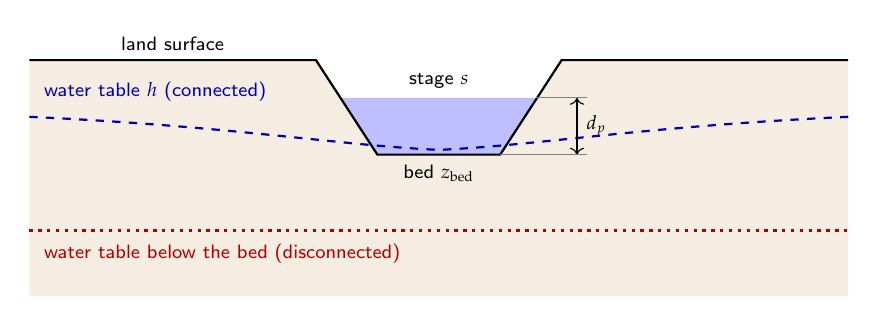
\begin{tikzpicture}[x=1.3cm,y=1.2cm,lab/.style={font=\scriptsize}]
\fill[brown!15] (-4,0) -- (4,0) -- (4,2.5) -- (1.2,2.5) -- (0.6,1.5) -- (-0.6,1.5) -- (-1.2,2.5) -- (-4,2.5) -- cycle;
\fill[blue!25] (-0.95,2.1) -- (0.95,2.1) -- (0.6,1.5) -- (-0.6,1.5) -- cycle;
\draw[thick] (-4,2.5) -- (-1.2,2.5) -- (-0.6,1.5) -- (0.6,1.5) -- (1.2,2.5) -- (4,2.5);
\draw[dashed,blue!70!black,thick] (-4,1.9) .. controls (-2,1.8) and (-1,1.6) .. (0,1.55) .. controls (1,1.6) and (2,1.8) .. (4,1.9);
\node[lab,blue!70!black,anchor=west] at (-3.95,2.17) {water table $h$ (connected)};
\draw[dotted,red!70!black,very thick] (-4,0.7) -- (4,0.7); \node[lab,red!70!black,anchor=west] at (-3.95,0.45) {water table below the bed (disconnected)};
\draw[<->] (1.35,1.5) -- (1.35,2.1); \node[lab,right] at (1.35,1.8) {$d_p$};
\draw[gray,thin] (0.6,1.5) -- (1.45,1.5); \draw[gray,thin] (0.95,2.1) -- (1.45,2.1);
\node[lab] at (0,2.28) {stage $s$}; \node[lab] at (0,1.3) {bed $z_{\mathrm{bed}}$};
\node[lab,anchor=south] at (-2.6,2.5) {land surface};
\end{tikzpicture}
\caption{River cell: stage $s$ = bed + Raven channel depth. With the water table above the bed, flow is $C(s-h)$ (either
direction); below the bed the river is disconnected and leaks at $C(s-z_{\mathrm{bed}})$.}\label{fig:river}
\end{figure}

\subsection{Never taking water the river does not have}
A losing river cannot give more than it carries. The conductance is therefore limited each day so that the largest
possible loss --- the disconnected rate $C(s-z_{\mathrm{bed}})$ --- is no more than the cell's share (by river length) of
the flow in the channel reach at the start of the day (the channel flow, upstream of any reservoir at the subbasin outlet):
\begin{equation}
C^{\mathrm{riv}}\le\frac{Q^{\mathrm{out}}_p\,(L_{p,i}/L_p)}{s-z_{\mathrm{bed}}},
\end{equation}
with $Q^{\mathrm{out}}_p$ in m$^3$/d and $L_p$ the subbasin's total river length on active cells. (Using the reservoir
release instead would cut off every river cell above a lake whenever the lake is not spilling.) Rivers of disabled
subbasins get no river cells.

\subsection{Back to Raven's rivers}
For each subbasin the net aquifer discharge is $G_p=-\sum_i q^{\mathrm{riv}}_{p,i}$ [m$^3$/d]. A gain is added to the
subbasin's in-catchment inflow for the day (so it passes Raven's catchment routing like other runoff). A loss is taken
first from that in-catchment inflow and then, inside Raven's routing loop, from the flow entering the reach from
upstream. A loss that still cannot be supplied in the day --- rare, because of the limit above --- is \emph{carried} to the
next day and taken from the river first thing then, so no water is created:
\begin{equation}
V^{\mathrm{applied}}_{p,n}=G_{p,n}\,\dt-K_{p,n-1}+K_{p,n},
\end{equation}
where $K_{p,n}$ [m$^3$] is the loss carried out of day $n$. Summed over a run, the water applied to Raven equals MODFLOW's net
river exchange minus whatever is still carried at the end (written to \cmd{solution.rvc} as \cmd{:GWRiverLossCarry} and
taken on the first day of a restart).
\begin{example}[: river exchange]
$K_b=0.5$ m/d, $M_b=1$ m, width 40 m, 2\,500 m of river in the cell: $C=0.5\times40\times2\,500/1=50\,000$ m$^2$/d. Bed
590 m, depth 1.5 m, stage 591.5 m. Water table at 590.8 m: $q=50\,000\times0.7=35\,000$ m$^3$/d lost to the aquifer.
Water table at 592.0 m: $q=-25\,000$ m$^3$/d, a gain for the river. Water table at 585 m (below the bed): the river
leaks $50\,000\times1.5=75\,000$ m$^3$/d.
\end{example}

\begin{refcard}{rivers}
\textbf{Sources/sinks.} Exchanges water in both directions between the aquifer (MODFLOW RIV package \cmd{RIV\_RAVEN} in every river cell) and Raven's
reaches: gains are added to the subbasin's in-catchment inflow; losses are taken from it and then from the reach inflow.\par\smallskip
\textbf{Constraints/notes.} The conductance is limited by the channel flow at the start of the step; a loss that cannot be supplied is carried to the next
step. The stage never exceeds the land surface; the bed is never above the model top. Disabled subbasins get no river cells.\par\smallskip
\par\noindent\begin{minipage}{\linewidth}\textbf{Command syntax}
\begin{lstlisting}
# .rvg
:RiverGeometry  my_rivers.geojson  SubId     # river lines; subbasin ID field optional
:RiverBedDepth  REFERENCE_FLOW               # or a depth [m] below the DEM
# .rvp
:AquiferProfileParameters
  :Attributes,     RIVERBED_K, RIVERBED_THICKNESS
  :Units,          m/d,        m
  VALLEY_ALLUVIUM, 0.5,        1.0
:EndAquiferProfileParameters
\end{lstlisting}
\end{minipage}\par\smallskip
\par\noindent\begin{minipage}{\linewidth}\textbf{Parameters}\par\smallskip
\begin{tabular}{>{\raggedright\arraybackslash}P{0.09\linewidth}>{\raggedright\arraybackslash}P{0.26\linewidth}>{\raggedright\arraybackslash}P{0.283\linewidth}>{\raggedright\arraybackslash}P{0.1\linewidth}>{\raggedright\arraybackslash}P{0.15\linewidth}}\toprule\hdr \hdr Symbol & Parameter & Class (where it is set) & Units & Reference\\\midrule
$K_b$ & \cmd{RIVERBED\_K} & aquifer profile (of the column) & m/d & Sec.~\ref{app:profile}\\
$M_b$ & \cmd{RIVERBED\_THICKNESS} & aquifer profile & m & Sec.~\ref{app:profile}\\
$W_p$, $d_p$ & channel top width, depth & subbasin channel (\cmd{:ChannelProfile}, \cmd{.rvp}); Raven routing state & m & Raven manual\\
$d_{\mathrm{bf},p}$ & \cmd{:RiverBedDepth} or depth at \cmd{Q\_REFERENCE} & \cmd{.rvg} option; subbasin parameter (\cmd{.rvh}) & m & Sec.~\ref{app:commands}\\
$L_{p,i}$ & river length in a cell & computed from \cmd{:RiverGeometry} & m & Sec.~\ref{ch:rivers}\\
$Q^{\mathrm{out}}_p$ & channel flow & Raven routing state (subbasin) & m$^3$/s & Raven state var.\\
\bottomrule\end{tabular}\end{minipage}\par\smallskip
\textbf{Outputs.} \cmd{GWBudget.csv}: \emph{river leakage to aquifer}, \emph{aquifer discharge to rivers}, \emph{river exchange applied to Raven},
\emph{river loss carried to next step}; streamflow in \cmd{Hydrographs.csv} includes the exchange.
\end{refcard}

\subsection{Common questions}
\textit{Why is the stage from the start of the step?} Raven routes rivers after MODFLOW has solved; using the start-of-step
depth avoids iterating between the two models, and at daily steps the difference is small. \textit{What if a subbasin has no
channel?} Its depth and width are zero, so its conductance and stage give no exchange, and any groundwater reaching the surface
there leaves through the seepage drains. \textit{Headwater reaches with little flow} cannot lose much water, because the supply
limit scales the conductance with the reach outflow.

\section{Evaporation from a shallow water table}\label{ch:et}
Plants and bare soil can draw water directly from a water table close to the surface. With the aquifer profile parameter \cmd{EXTINCTION\_DEPTH} (Section~\ref{app:profile})
$d_x>0$, each active column gets MODFLOW's EVT package. Raven first satisfies evaporation from its own stores; only the
potential evaporation it could \emph{not} meet is offered to the water table:
\begin{equation}
E_i=\frac{1}{\Delta^2}\sum_kA_{k,i}\;\frac{\max\left(\mathrm{PET}_k\,\dt-\mathrm{AET}_k,\;0\right)}{1000\,\dt}\quad[\mathrm{m/d}],
\end{equation}
where $\mathrm{PET}_k$ [mm/d] is the HRU's potential evaporation and $\mathrm{AET}_k$ [mm] what Raven already evaporated
that day. Only HRUs whose own profile has an extinction depth contribute. The unmet demand of those HRUs in the cell (a volume) is spread over the whole cell area $\Delta^2$, because MODFLOW
multiplies the rate by the full cell area. The most MODFLOW can remove is then exactly that unmet volume, even where coupled
HRUs cover only part of the cell. MODFLOW removes
\begin{equation}
Q^{\mathrm{evt}}_i=E_i\,\Delta^2\;\min\!\left(1,\max\!\left(0,\;1-\frac{z_{\mathrm{land},i}-h_i}{d_x}\right)\right),
\end{equation}
the full rate when the water table is at the surface, falling linearly to zero at depth $d_x$ (Figure~\ref{fig:curves}d).
This water leaves the system as evaporation.
\begin{example}[: water-table ET]
Unmet PET 2 mm/d over a 4 km$^2$ cell fully covered by coupled HRUs, $d_x=2$ m, water table 0.5 m deep:
$Q=0.002\times4\times10^6\times(1-0.5/2)=6\,000$ m$^3$/d. If coupled HRUs covered only 1 km$^2$ of the cell, the unmet volume
would be 2\,000 m$^3$, $E=2\,000/4\times10^6=0.5$ mm/d over the cell, and $Q=1\,500$ m$^3$/d.
\end{example}

\begin{refcard}{water-table evaporation}
\textbf{Sources/sinks.} Moves water from the aquifer (MODFLOW EVT package \cmd{EVT\_RAVEN}, top cell) to the atmosphere. It leaves the system and is
not included in Raven's \cmd{AET}.\par\smallskip
\textbf{Constraints/notes.} Only HRUs whose aquifer profile has an extinction depth contribute; MODFLOW can never remove more than their unmet
evaporative demand; the rate falls linearly to zero at the extinction depth.\par\smallskip
\par\noindent\begin{minipage}{\linewidth}\textbf{Command syntax}
\begin{lstlisting}
# .rvp
:AquiferProfileParameters
  :Attributes,     EXTINCTION_DEPTH
  :Units,          m
  VALLEY_ALLUVIUM, 2.0
:EndAquiferProfileParameters
\end{lstlisting}
\end{minipage}\par\smallskip
\par\noindent\begin{minipage}{\linewidth}\textbf{Parameters}\par\smallskip
\begin{tabular}{>{\raggedright\arraybackslash}P{0.09\linewidth}>{\raggedright\arraybackslash}P{0.26\linewidth}>{\raggedright\arraybackslash}P{0.283\linewidth}>{\raggedright\arraybackslash}P{0.1\linewidth}>{\raggedright\arraybackslash}P{0.15\linewidth}}\toprule\hdr \hdr Symbol & Parameter & Class (where it is set) & Units & Reference\\\midrule
$d_x$ & \cmd{EXTINCTION\_DEPTH} & aquifer profile (0 = off) & m & Sec.~\ref{app:profile}\\
$\mathrm{PET}_k$ & potential evapotranspiration & Raven forcing function of HRU $k$ (\cmd{:Evaporation} method, \cmd{.rvi}) & mm/d & Raven manual\\
$\mathrm{AET}_k$ & \cmd{AET} & Raven state variable of HRU $k$ & mm & Raven state var.\\
\bottomrule\end{tabular}\end{minipage}\par\smallskip
\textbf{Outputs.} \cmd{GWBudget.csv}: \emph{water-table ET}. Total evaporation is Raven's AET plus this column.
\end{refcard}

\section{Wetlands and lakes held in Raven stores}\label{ch:stores}
Wetlands and small lakes are often represented in Raven by a store in their HRUs: \cmd{DEPRESSION} for wetlands, or
\cmd{LAKE\_STORAGE} for lakes. \cmd{:SurfaceWater\allowbreak Exchange SV group LEAKANCE L} connects such a store, in the HRUs of an HRU
group, to the aquifer below.

\subsection{The boundary}
In each column holding HRUs of the group, the exchange is a river-type boundary (MODFLOW RIV package) whose bed is the
model top and whose water level is the top plus the average depth of water in the store:
\begin{equation}
\bar s_i=\frac{\sum_kA_{k,i}\,s_k}{\sum_kA_{k,i}},\qquad h_b=z_{\mathrm{top},i}+\bar s_i,
\qquad q=\begin{cases}C\left(h_b-h\right) & h>z_{\mathrm{top},i},\\ C\,\bar s_i & h\le z_{\mathrm{top},i},\end{cases}
\end{equation}
with $s_k$ the store depth of HRU $k$ in metres ($1/1000$ of the store in mm). Positive $q$ is leakage from the store to
the aquifer; negative $q$ is groundwater feeding the store. Because leakage stops growing once the water table is below
the store's bed, it can never exceed $C\,\bar s_i$.

\subsection{Never draining more than the store holds}
The water available in a cell is the store's real volume, split among the HRU's cells by overlap and fixed at the start
of the day:
\begin{equation}
V_{k,i}=s_k\,A_k\,\frac{A_{k,i}}{\sum_jA_{k,j}},\qquad V_i=\sum_kV_{k,i} .
\end{equation}
The conductance is limited so that the largest possible leakage in the day is no more than this water:
\begin{equation}
C=\min\!\left(L\sum_kA_{k,i},\ \frac{V_i}{\dt\,\bar s_i}\right),\qquad C=0\ \text{when the stores are empty}.
\end{equation}
After MODFLOW solves, leakage is removed from each HRU's store in proportion to $V_{k,i}$, and groundwater discharge is
added in proportion to area. Because the shares come from the same fixed volumes used for the limit, no store can be
over-drawn and the volumes on both sides match exactly. A store of an HRU may be connected by only one
\cmd{:SurfaceWater\allowbreak Exchange}; Raven stops if two exchanges would draw on the same store. Groundwater that reaches the surface under an \emph{empty} store is
still returned to Raven by the seepage drain (Section~\ref{ch:seepage}).
\begin{example}[: wetland leakage]
Group HRUs cover 3 km$^2$ of a cell, $L=0.05$ d$^{-1}$: $C\le0.05\times3\times10^6=150\,000$ m$^2$/d. The wetland holds
20 mm ($\bar s=0.02$ m, $V=60\,000$ m$^3$ in this cell). The supply limit is $60\,000/(1\times0.02)=3\times10^6$ m$^2$/d, so
$C=150\,000$. With the water table 1 m below the top (disconnected), leakage is $150\,000\times0.02=3\,000$ m$^3$/d, i.e.\
1 mm/d over the 3 km$^2$.
\end{example}

\begin{refcard}{wetlands and lakes}
\textbf{Sources/sinks.} Exchanges water in both directions between a Raven storage state variable (e.g.\ \cmd{DEPRESSION}, \cmd{LAKE\_STORAGE},
\cmd{SOIL[0]}) of the HRUs in an HRU group and the aquifer (MODFLOW RIV package \cmd{SWX\_RAVEN}, top cell).\par\smallskip
\textbf{Constraints/notes.} The conductance is limited by the water stored, so a store can never be over-drawn; an empty store does not leak. A store of
an HRU may be connected by one exchange only.\par\smallskip
\par\noindent\begin{minipage}{\linewidth}\textbf{Command syntax}
\begin{lstlisting}
# .rvg
:SurfaceWaterExchange  DEPRESSION  WetlandHRUs  LEAKANCE 0.01
# .rvh
:HRUGroup WetlandHRUs
  101, 102, 157
:EndHRUGroup
\end{lstlisting}
\end{minipage}\par\smallskip
where \cmd{DEPRESSION} is the Raven store, \cmd{WetlandHRUs} an HRU group and 0.01 the leakance [1/d].
\par\smallskip\noindent\begin{minipage}{\linewidth}\textbf{Parameters}\par\smallskip
\begin{tabular}{>{\raggedright\arraybackslash}P{0.09\linewidth}>{\raggedright\arraybackslash}P{0.26\linewidth}>{\raggedright\arraybackslash}P{0.283\linewidth}>{\raggedright\arraybackslash}P{0.1\linewidth}>{\raggedright\arraybackslash}P{0.15\linewidth}}\toprule\hdr \hdr Symbol & Parameter & Class (where it is set) & Units & Reference\\\midrule
$L$ & \cmd{LEAKANCE} & \cmd{:SurfaceWater\allowbreak Exchange} argument (\cmd{.rvg}) & 1/d & Sec.~\ref{app:commands}\\
$s_k$ & store depth & Raven state variable (the named store) of HRU $k$ & mm & Raven state var.\\
-- & HRU group & \cmd{:HRUGroup} (\cmd{.rvh}) & -- & Raven manual\\
\bottomrule\end{tabular}\end{minipage}\par\smallskip
\textbf{Outputs.} \cmd{GWBudget.csv}: \emph{surface-store leakage to aquifer}, \emph{aquifer discharge to surface stores}, \emph{surface-store
exchange applied to Raven}; the store itself in Raven's outputs.
\end{refcard}

\section{Reservoirs}\label{ch:reservoirs}
Raven reservoirs can already lose water to groundwater with their \cmd{:SeepageParameters} $k$ [m$^3$/s/m] and a fixed
local groundwater level $h_{\mathrm{loc}}$:
\begin{equation}
V^{\mathrm{res}}=k\left(\tfrac12\left(h^{t}_{\mathrm{res}}+h^{t+\dt}_{\mathrm{res}}\right)-h_{\mathrm{loc}}\right)\cdot86\,400\,\dt
\quad[\mathrm{m}^3],
\end{equation}
using the average of the stages at the start and end of the step. \cmd{:ReservoirExchange} connects this to the aquifer
for every reservoir that has \cmd{:SeepageParameters} and whose lake HRU (\cmd{:HRUID}) has an \cmd{AQUIFER\_PROFILE}.

\subsection{How the exchange works}
\begin{enumerate}
\item After MODFLOW solves a day, the local groundwater level of the reservoir is set to the average head under its
lake HRU, weighted by overlap:
\begin{equation}
h_{\mathrm{loc}}=\sum_iw_i\,\max\!\left(z^{\mathrm{wt}}_i,\;\min\!\left(z_{\mathrm{top},i},\,h_{\mathrm{res}}\right)\right),\qquad w_i=\frac{A_{k,i}}{\sum_{j\notin\mathcal{C}}A_{k,j}} ,
\end{equation}
where the sums run over the lake HRU's cells that do not hold a fixed head ($\mathcal{C}$), as for recharge, and
$z^{\mathrm{wt}}_i$ is the water table of column $i$ (the head of its highest wet cell; Section~\ref{ch:mf6}). A water table
below the lake bed (the model top) means the lake is disconnected: its seepage then depends on the bed, not on how deep
the water table is --- exactly as for a river. If the lake stands below the model top (for example a DEM that recorded a
higher water surface), the true bed is below the lake level, so the bed is taken at the lake level $h_{\mathrm{res}}$: a
deep water table then gives no exchange, where the model top would have given a false inflow to the lake. (Using raw heads
here was an error: a dry cell's head can be far below the cell and produced impossible seepage.)
\item Raven routes the day; the reservoir calculates its seepage $V^{\mathrm{res}}$ with this level and counts it as a
reservoir loss (water leaving Raven).
\item The next day, this volume is injected into the aquifer cells under the lake (MODFLOW WEL package
\cmd{RES\_RAVEN}): $Q_i=V^{\mathrm{res}}\,w_i/\dt$. A negative volume (groundwater feeding the reservoir) is extracted.
If a cell is nearly dry, MODFLOW extracts less than asked (\cmd{AUTO\_FLOW\_REDUCE}); the lake has already received that
water, so the shortfall is taken back from the water reaching the reservoir's subbasin in the same step, like a river loss
(\cmd{GWBudget.csv}: \emph{reservoir gain not supplied by MODFLOW}). No water is created.
\end{enumerate}
The reservoir's stages must be elevations on the aquifer's datum (\cmd{:AbsoluteCrest\allowbreak Height}): a stage below the
bottom of the whole aquifer under the lake --- relative stages, with the crest at 0 m, or another datum --- stops the run.
For a large lake, fine cells in and around the lake HRU place this seepage more precisely: \cmd{:GridRefinement LAKES}
(Section~\ref{sec:gridtypes}). The one-day delay is exact bookkeeping, not a loss. The volume in transit is reported every day (\emph{reservoir seepage
awaiting delivery}), saved in \cmd{solution.rvc} (\cmd{:GWReservoirSeepage}), and delivered on the first day of a
restarted run.

Without an initial condition in the \cmd{.rvc}, a reservoir with absolute stages starts at its crest height --- the same state
that stage 0 means for a reservoir with relative stages. (Raven previously started it at 0~m, far below the lake bed,
which created a large one-time error in its water balance; this was corrected.) Stages count as absolute when
\cmd{:AbsoluteCrest\allowbreak Height} is given or when a stage--storage table starts above 0~m; a table measured from the
reservoir bottom that happens to start above 0~m therefore also starts at the crest, so give such reservoirs an
\cmd{:InitialReservoirStage}.
\begin{watch}
The reservoir stage and the aquifer heads must use the same vertical datum. Give reservoirs absolute elevations (for
simple lakes, \cmd{:AbsoluteCrest\allowbreak Height}).
\end{watch}
\begin{example}[: reservoir seepage]
$k=0.2$ m$^3$/s/m, average stage 1\,136 m, aquifer head below the lake 1\,132 m: seepage
$0.2\times4\times86\,400=69\,120$ m$^3$ that day, injected into the aquifer the next day.
\end{example}

\begin{refcard}{reservoirs}
\textbf{Sources/sinks.} Exchanges water between a Raven reservoir (subbasin outlet) and the aquifer under its lake HRU (MODFLOW WEL package
\cmd{RES\_RAVEN}); Raven books the seepage as a reservoir loss.\par\smallskip
\textbf{Constraints/notes.} One-step lag, exactly accounted (volume in transit reported and saved). The local head is never taken below the lake bed.
Stages must be absolute. A reservoir that dries out books only the water that can actually leave.\par\smallskip
\par\noindent\begin{minipage}{\linewidth}\textbf{Command syntax}
\begin{lstlisting}
# .rvh
:Reservoir Lake1
  :SubBasinID          43
  :HRUID               2736      # lake HRU, with an AQUIFER_PROFILE
  :Type                RESROUTE_STANDARD
  :WeirCoefficient     0.6
  :CrestWidth          100.0
  :MaxDepth            10.0
  :LakeArea            5.0E7
  :AbsoluteCrestHeight 1133.0    # absolute stages (required)
  :SeepageParameters   0.2 1128  # k [m3/s/m]; the head is replaced by the aquifer head
:EndReservoir
# .rvg
:ReservoirExchange
\end{lstlisting}
\end{minipage}\par\smallskip
\par\noindent\begin{minipage}{\linewidth}\textbf{Parameters}\par\smallskip
\begin{tabular}{>{\raggedright\arraybackslash}P{0.09\linewidth}>{\raggedright\arraybackslash}P{0.26\linewidth}>{\raggedright\arraybackslash}P{0.283\linewidth}>{\raggedright\arraybackslash}P{0.1\linewidth}>{\raggedright\arraybackslash}P{0.15\linewidth}}\toprule\hdr \hdr Symbol & Parameter & Class (where it is set) & Units & Reference\\\midrule
$k$ & \cmd{:SeepageParameters} (first value) & reservoir (\cmd{:Reservoir}, \cmd{.rvh}) & m$^3$/s/m & Raven manual\\
$h_{\mathrm{res}}$ & stage & Raven reservoir state; \cmd{:AbsoluteCrest\allowbreak Height} & m & Raven state var.\\
$h_{\mathrm{loc}}$ & local groundwater head & computed each step from MODFLOW (replaces the second value) & m & Sec.~\ref{ch:reservoirs}\\
-- & \cmd{:ReservoirExchange} & \cmd{.rvg} option & -- & Sec.~\ref{app:commands}\\
\bottomrule\end{tabular}\end{minipage}\par\smallskip
\textbf{Outputs.} \cmd{GWBudget.csv}: \emph{reservoir seepage sent}, \emph{delivered}, \emph{awaiting delivery}, \emph{reservoir gain not supplied by MODFLOW}; Raven's reservoir outputs show
the seepage as a loss.
\end{refcard}

\section{Wells and boundaries}\label{ch:wells}
\subsection{Pumping and injection wells}
Wells are listed in \cmd{:Wells} with their location and screen (top and bottom elevation); pumping rates come from a
time series \cmd{:WellRate} in the \cmd{.rvt} file (m$^3$/d, negative for pumping). A screen that crosses several layers
is split among them by transmissivity, so more water comes from the more permeable layers:
\begin{equation}
Q_{w,\ell}=Q_w\,\frac{T_\ell}{\sum_mT_m},\qquad
T_\ell=K_\ell\left[\min\!\left(z_{\mathrm{st}},z^{(\ell-1)}_{\mathrm{bot}}\right)-\max\!\left(z_{\mathrm{sb}},z^{(\ell)}_{\mathrm{bot}}\right)\right]_+,
\end{equation}
where $[x]_+=\max(x,0)$ and $z_{\mathrm{st}},z_{\mathrm{sb}}$ are the screen top and bottom. If the screen misses the
aquifer, the nearest active layer is used (with a warning). MODFLOW's \cmd{AUTO\_FLOW\_REDUCE} lowers the pumping rate as a cell runs dry, so a well cannot pump water that is not
there. A well placed in a fixed-head cell has no effect, and Raven warns about it. \cmd{GWBudget.csv} reports both the
specified and the actual rates. Pumped water leaves the system.

\subsection{Head-dependent boundaries (GHB)}
A general-head boundary exchanges water with a water body outside the model --- for example a large lake or the
continuation of the aquifer beyond the model:
\begin{equation}
q=C_g\left(h_g-h\right),
\end{equation}
with $C_g$ the conductance per cell (\cmd{CONDUCTANCE}) and $h_g$ the boundary head (\cmd{HEAD}, or a \cmd{:BoundaryHead}
time series).

\subsection{Fixed-head boundaries (CHD)}
A specified-head boundary holds the head of its cells at $h_c$; MODFLOW calculates whatever flow is needed to do so.

\subsection{Where boundaries go}
Boundaries are drawn in a GeoJSON file: polygons select the cells whose centre lies inside (tested with the even--odd
ray-crossing rule, so holes work), lines select the cells they cross. With \cmd{LAYERS TOP} only the top active cell
is used; with \cmd{LAYERS ALL}, every active layer. A boundary is placed only in cells whose bottom is below its head
(MODFLOW requires this), and time-varying heads are kept at least 0.01 m above the cell bottom.

\subsection{Monitoring (observation) wells}
Monitoring wells are listed in \cmd{:ObservationWells} with a location and a screen elevation. Each is attached to the
active cell of its column whose layer contains the screen elevation (or the nearest active layer). Their simulated heads
are written to \cmd{GWHeads.csv} and can be compared with measurements through \cmd{:ObservationData} or
\cmd{:IrregularObservations GW\_HEAD} (matched to the observation times like any Raven observation, within \cmd{:EvaluationTime}) in the
\cmd{.rvt} file; Raven then computes the usual goodness-of-fit statistics (NSE, RMSE, KGE, \dots) in \cmd{Diagnostics.csv}.

\begin{refcard}{wells, boundaries and monitoring wells}
\textbf{Sources/sinks.} Wells: between the aquifer (MODFLOW WEL package \cmd{WEL\_RAVEN}) and the outside. General-head boundaries (GHB
\cmd{GHB\_RAVEN}): between the aquifer and an external water body. Fixed heads (CHD \cmd{CHD\_RAVEN}): whatever flow holds the
head. Monitoring wells move no water.\par\smallskip
\textbf{Constraints/notes.} Pumping is reduced automatically as a cell runs dry (\cmd{AUTO\_FLOW\_REDUCE}); a well in a fixed-head cell has no effect
(warning). Boundary heads are kept above cell bottoms. Duplicate IDs and names are rejected.\par\smallskip
\par\noindent\begin{minipage}{\linewidth}\textbf{Command syntax}
\begin{lstlisting}
# .rvg
:Wells
  :Attributes, NAME, LATITUDE, LONGITUDE, SCREEN_TOP, SCREEN_BOT
  1, PW_1, 59.27309, -124.73461, 1199.7, 1188.7
:EndWells
:ObservationWells
  :Attributes, NAME, LATITUDE, LONGITUDE, SCREEN_ELEV
  101, OW_1, 59.27310, -124.73060, 1192.7
:EndObservationWells
:GeneralHeadBoundary   G1  edge.geojson  HEAD 1146.9 CONDUCTANCE 5000 LAYERS TOP
:SpecifiedHeadBoundary L1  lake.geojson  HEAD 1226.5 LAYERS TOP
# .rvt
:WellRate 1 m3/d                 # negative = pumping
  1985-10-01 00:00:00 1.0 3
  -1000.0
  -1000.0
  -1200.0
:EndWellRate
:ObservationData GW_HEAD 101 m   # observed heads
  ...
:EndObservationData
\end{lstlisting}
\end{minipage}\par\smallskip
\par\noindent\begin{minipage}{\linewidth}\textbf{Parameters}\par\smallskip
\begin{tabular}{>{\raggedright\arraybackslash}P{0.09\linewidth}>{\raggedright\arraybackslash}P{0.26\linewidth}>{\raggedright\arraybackslash}P{0.283\linewidth}>{\raggedright\arraybackslash}P{0.1\linewidth}>{\raggedright\arraybackslash}P{0.15\linewidth}}\toprule\hdr \hdr Symbol & Parameter & Class (where it is set) & Units & Reference\\\midrule
$Q_w$ & \cmd{:WellRate} & time series (\cmd{.rvt}) & m$^3$/d & Sec.~\ref{app:commands}\\
$z_{\mathrm{st}}$, $z_{\mathrm{sb}}$ & \cmd{SCREEN\_TOP}, \cmd{SCREEN\_BOT} & \cmd{:Wells} table (\cmd{.rvg}) & m & Sec.~\ref{app:commands}\\
$K_\ell$ & \cmd{K\_HORIZ} & aquifer class of layer $\ell$ & m/d & Sec.~\ref{app:class}\\
$C_g$ & \cmd{CONDUCTANCE} & \cmd{:GeneralHeadBoundary} (\cmd{.rvg}) & m$^2$/d & Sec.~\ref{app:commands}\\
$h_g$, $h_c$ & \cmd{HEAD} or \cmd{:BoundaryHead} & \cmd{.rvg} command; time series (\cmd{.rvt}) & m & Sec.~\ref{app:commands}\\
-- & \cmd{SCREEN\_ELEV} & \cmd{:ObservationWells} (\cmd{.rvg}) & m & Sec.~\ref{app:commands}\\
\bottomrule\end{tabular}\end{minipage}\par\smallskip
\textbf{Outputs.} \cmd{GWBudget.csv}: \emph{wells specified}, \emph{wells actual}, \emph{GHB}, \emph{CHD}; \cmd{GWHeads.csv}; \cmd{GW\_HEAD}
statistics in \cmd{Diagnostics.csv}.
\end{refcard}

\subsection{Where does pumped water come from?}
At first mostly from aquifer storage (a cone of depression forms); as the cone reaches rivers and seepage areas, more and more
comes from reduced discharge to streams (``capture''). In the Liard pumping test 91\% of the pumping was captured from reduced discharge to rivers in the first year and 98\% in the
fifth, and the outflow downstream fell by 98\% of the pumping rate.

\chapter{Water accounting and time stepping}\label{ch:c5}
This chapter explains how the two models keep their water accounts consistent, what exactly happens in each time step,
and how runs are started, restarted and repeated.

\begin{plain}
Every day the two models take turns: Raven works out how much water goes down; MODFLOW moves it through the aquifer and
reports what comes back up; Raven then books the returned water. Both keep a running account, and the two accounts are
compared every day. This chapter also explains how to stop a run and carry on later (a restart), and how to run many
versions of a model at once (an ensemble).
\end{plain}

\section{Keeping the books: water balance}\label{ch:balance}
\subsection{MODFLOW's balance}
For every step Raven computes all boundary flows from MODFLOW's own matrix terms ($q=\mathrm{HCOF}\cdot h-\mathrm{RHS}$)
and the storage change from MODFLOW's storage package, and reports the imbalance
\begin{multline}
\varepsilon=Q^{\mathrm{rch}}+Q^{\mathrm{sto}}-Q^{\mathrm{seep}}+Q^{\mathrm{riv}}_{\mathrm{in}}-Q^{\mathrm{riv}}_{\mathrm{out}}-Q^{\mathrm{evt}}
+Q^{\mathrm{wel}}+Q^{\mathrm{ghb}}+Q^{\mathrm{chd}}\\+Q^{\mathrm{swx}}_{\mathrm{in}}-Q^{\mathrm{swx}}_{\mathrm{out}}+Q^{\mathrm{res}},
\end{multline}
where $Q^{\mathrm{sto}}$ is water released from storage. It is written in m$^3$/d and as a percentage of the gross flow
(the sum of the absolute values of all terms). In the tests of Chapter~\ref{ch:verification} the worst single-day error is about $5\times10^{-6}$\% and the
cumulative error about $10^{-10}$.

\subsection{Raven's balance}
Raven tracks cumulative input $I$ and output $O$ and reports $\mathrm{MB}=\left(S-S_0\right)+\left(O-I\right)$ in mm over
the watershed. The coupling adds:
\begin{itemize}
\item \textbf{to output}: recharge (the end-of-day \cmd{GROUNDWATER} value of coupled HRUs, as Raven already does), and
reservoir seepage (already counted by Raven as a reservoir loss);
\item \textbf{to input}: every volume the coupling adds to Raven in the step --- seepage returned to HRU stores, the net
river exchange applied to reaches, and the net surface-store exchange. A net loss (for example a losing river) is a
negative input.
\end{itemize}
With these, Raven's own balance closes exactly as without groundwater (0.43--0.52 mm maximum over 20 years in the Liard
example, the same as uncoupled).

\subsection{The whole system}
The water that leaves Raven as recharge enters MODFLOW (directly or via the delay store); the water MODFLOW sends back
enters Raven. Reservoir seepage enters MODFLOW one day after leaving Raven. Therefore
\begin{equation}
\sum V^{\mathrm{Raven}}_{\mathrm{rch}}=\sum V^{\mathrm{MF6}}_{\mathrm{rch}}+\Delta S^{\mathrm{delay}}+\sum V^{\mathrm{CHD}}_{\mathrm{rch}},
\end{equation}
and the audit tool checks this identity, the river, seepage and store bookkeeping, and MODFLOW's balance for every run.

\section{A real day of water accounts}
\begin{example}[: 15 June 1996 in the Liard run]
From \cmd{GWBudget.csv} (all in m$^3$/d):
\begin{center}\begin{tabular}{lr}\toprule\hdr
Inflows to the aquifer & \\\midrule
recharge from Raven & 21\,365\,037\\
river leakage & 2\,978\,677\\\midrule\hdr
Outflows from the aquifer & \\\midrule
seepage to Raven & 19\,087\,047\\
discharge to rivers & 1\,331\,456\\\midrule
storage release (negative = stored) & $-$3\,925\,212\\\bottomrule
\end{tabular}\end{center}
Inflows $-$ outflows $+$ release $=24\,343\,714-20\,418\,502-3\,925\,212=0.00003$ m$^3$/d, i.e.\ a relative error of
about $10^{-10}$. Raven recorded the same numbers on its side: 21.4 million m$^3$ of recharge leaving its stores, 19.1 million m$^3$
of seepage entering them, and a net river exchange of $-1.65$ million m$^3$ applied to its reaches (the rivers lost more than
they gained that day). The aquifer stored the difference: a water-table rise of about 1 mm on average.
\end{example}

\section{How to read the balance outputs}
\begin{enumerate}
\item \emph{MF6 balance error [\%]} should stay well below 0.1\% every step; larger values point to a non-converged step or a
too-loose head tolerance (\cmd{:SolverHead\allowbreak Tolerance}, default 0.00001 m).
\item \emph{Raven recharge} and \emph{MF6 recharge} are equal unless a recharge delay or fixed-head cells are used.
\item \emph{returned to Raven} equals \emph{seepage to Raven}.
\item \emph{river loss carried to next step} is normally zero; when not, it is taken from the river the next day.
\item Raven's \cmd{Watershed\allowbreak Storage.csv} MB error should be as small as without groundwater.
\end{enumerate}
The tool \cmd{tools\_audit.py} checks all of these automatically.

\section{The coupled time step, start-up and restarts}\label{ch:timestep}
\subsection{The algorithm}
\begin{figure}[!htbp]\centering
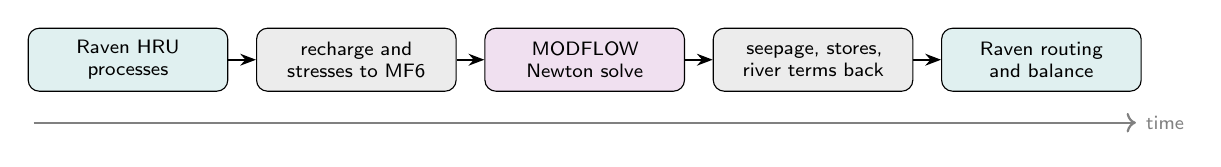
\begin{tikzpicture}[x=1cm,y=1cm,b/.style={draw,rounded corners,font=\scriptsize,align=center,minimum height=8mm,text width=23mm}]
\node[b,fill=teal!12] (a) at (0,0) {Raven HRU\\processes};
\node[b,fill=gray!15] (b) at (2.9,0) {recharge and\\stresses to MF6};
\node[b,fill=violet!12] (c) at (5.8,0) {MODFLOW\\Newton solve};
\node[b,fill=gray!15] (d) at (8.7,0) {seepage, stores,\\river terms back};
\node[b,fill=teal!12] (e) at (11.6,0) {Raven routing\\and balance};
\foreach \u/\v in {a/b,b/c,c/d,d/e} \draw[-{Stealth[length=2mm]},thick] (\u) -- (\v);
\draw[->,thick,gray] (-1.2,-0.8) -- (12.8,-0.8) node[right,font=\scriptsize]{time};
\end{tikzpicture}
\caption{Order of work within one time step.}\label{fig:timeline}
\end{figure}

Algorithm~\ref{alg:step} lists exactly what happens in one Raven time step of a coupled model.

\begin{algorithm}[h]\caption{One coupled time step}\label{alg:step}
\begin{algorithmic}[1]
\State Raven: vertical and lateral processes of all HRUs; coupled HRUs' \cmd{GROUNDWATER} now holds the day's recharge
\State Complete yesterday's line of \cmd{GWBudget.csv} (river and reservoir terms are final only after routing)
\State Recharge: delay reservoirs (Ch.~\ref{ch:recharge}); spread over cells; skip fixed-head cells
\State MODFLOW \cmd{prepare\_time\_step}; set RCH rates
\State Set river stages and conductances, well rates, GHB/CHD heads (Ch.~\ref{ch:rivers},\ref{ch:wells})
\State Set water-table ET rates from PET left unmet by Raven (Ch.~\ref{ch:et})
\State Deliver yesterday's reservoir seepage (Ch.~\ref{ch:reservoirs}); set surface-store levels and limited conductances (Ch.~\ref{ch:stores})
\State MODFLOW \cmd{prepare\_solve}; \textbf{repeat} \cmd{solve} \textbf{until} converged or the iteration limit; \cmd{finalize\_solve}; \cmd{finalize\_time\_step}
\State Compute every package flow as $\mathrm{HCOF}\cdot h-\mathrm{RHS}$; reservoir local heads for today's routing
\State Surface-store exchange applied to Raven stores; seepage and river flows computed
\If{the step did not converge} limit seepage and river gains returned to Raven to the step's total inflow; warn \EndIf
\State Seepage added to Raven stores; balance, heads, connectivity and NetCDF output written
\State Raven: before routing, river gains added to / losses taken from each subbasin's in-catchment inflow
\State Raven routing; losses not covered are taken from the flow entering each reach; reservoirs compute seepage
\State Raven: water balance (recharge out, all returned water in); diagnostics including \cmd{GW\_HEAD}
\end{algorithmic}
\end{algorithm}

\subsection{Starting conditions}\label{sec:init}
Initial heads are chosen in this order: (1) a hotstart block \cmd{:GWHeads} in the \cmd{.rvc} file; (2)
\cmd{:InitialGWHeads} in the \cmd{.rvc} file (\cmd{DEPTH\_BELOW\_SURFACE d} or \cmd{ELEVATION z}); (3) each profile's
\cmd{INITIAL\_HEAD\_DEPTH}. Guessed initial heads can be far from reality; \cmd{:GWInitialization STEADY\_STATE r}
first solves a steady state before Raven's first day, with recharge $r$ [mm/d] over the area covered by coupled HRUs
(cell $i$ receives $r\,a_i/1000$ m$^3$/d) and the initial river stages, well rates and boundary heads. This is skipped on a hotstart. A steady state may not
exist --- for example when wells pump more than the aquifer can supply --- and then the solve does not converge; Raven
warns and starts from the initial heads instead, as if \cmd{:GWInitialization} had not been given. The groundwater model is built after \emph{all} input files,
including the \cmd{.rvc}, have been read.

\subsection{Restarting a run (hotstart)}
At the end of a run Raven writes \cmd{solution.rvc}. Besides Raven's own states it contains \cmd{:GWHeads} (the head in
every cell), \cmd{:GWRechargeStore} (recharge delay stores, if used), \cmd{:GWRiverLossCarry} (river loss carried, if any) and \cmd{:GWReservoirSeepage} (reservoir seepage in
transit, if used). Using this file as the \cmd{.rvc} of a new run --- with \cmd{:StartDate} set to the end of the first
run --- continues exactly: in the tests the restarted run matched a continuous run to within $6\times10^{-6}$ in all flows.

\subsection{Ensembles}
Raven's ensemble modes (Monte Carlo, DDS, EnKF) run the model several times in one program run. For every member the
groundwater model is rebuilt from scratch, MODFLOW is restarted, and its files go to that member's output folder.
Raven itself was corrected so that each member starts with a fresh water balance and, unless its own \cmd{.rvc} says
otherwise, from the routing memory and reservoir states of the first run (stage, outflow, loss terms). These defaults are
restored before the member's \cmd{.rvc} is read, so member-specific initial conditions (as used by EnKF forecasting) still
apply; groundwater hotstart values are likewise cleared, so each member uses only its own \cmd{.rvc}, and the steady-state
start is decided for each member separately
(Section~\ref{sec:coreflix}).

\subsection{Safeguards}\label{sec:guard}
\begin{itemize}
\item \textbf{Non-converged steps.} All water returned to Raven in such a step (seepage plus river gains) is limited to
the water that entered the aquifer in that step (recharge, river and store leakage, reservoir injection and boundary
inflows); discharge into wetland and lake stores is limited the same way. The step is flagged and a warning written.
\item \textbf{Rivers and stores} can never lose more water than they hold (Sections~\ref{ch:rivers},\ref{ch:stores}).
\item \textbf{Wells} cannot pump from a dry cell (\cmd{AUTO\_FLOW\_REDUCE}).
\item \textbf{Step count}: Raven stops if it would run past MODFLOW's last step.
\item \textbf{MODFLOW folder}: if Raven cannot enter the MODFLOW folder, the call fails with a clear message instead of
running MODFLOW in the wrong place.
\end{itemize}

\chapter{Inputs and outputs}\label{ch:c6}
This chapter is the reference for every command and every output, followed by a complete example set-up.

\begin{plain}
This is the look-up chapter: every command you can write in the input files, what it does and its default, and every output
file with its columns. There is no need to read it from start to finish; come here when you need the exact spelling of a
command or the meaning of an output column.
\end{plain}

\section{Input reference}\label{ch:inputs}
This chapter lists every command. Commands are case sensitive; separators may be commas or spaces, as in all Raven files.

\subsection{\texttt{.rvi} (main input file)}
\begin{table}[!htbp]\centering
\caption{Commands in the \cmd{.rvi} file.}
\begin{tabular}{P{0.34\linewidth}P{0.608\linewidth}}\toprule\hdr
Command & Meaning\\\midrule
\cmd{:GroundwaterModel MODFLOW6} & switches the coupling on (\cmd{NONE}: off, the default)\\
\cmd{:rvg\_Filename file} & name of the groundwater file, relative to the \cmd{.rvi} (default \cmd{<model>.rvg})\\
processes into \cmd{GROUNDWATER} & any process moving water into \cmd{GROUNDWATER} in a coupled HRU produces recharge; use
\cmd{:-->Conditional HRU\_GROUP} so uncoupled HRUs keep their own baseflow\\\bottomrule
\end{tabular}
\end{table}

\subsection{\texttt{.rvh} (HRUs and subbasins)}
The existing \cmd{AQUIFER\_PROFILE} column of \cmd{:HRUs} holds a profile name, or \cmd{[NONE]}. Reservoirs to be coupled
need \cmd{:SeepageParameters} and a lake HRU (\cmd{:HRUID}) with an \cmd{AQUIFER\_PROFILE}.

\subsection{\texttt{.rvp} (parameters)}
\begin{lstlisting}
:AquiferClasses
  :Attributes, K_HORIZ, K_VERT, SPEC_STORAGE, SPEC_YIELD, POROSITY
  :Units,      m/d,     m/d,    1/m,          none,       none
  GRAVEL,      50.0,    5.0,    1.0E-5,       0.25,       0.30
  CLAY_TILL,   0.001,   0.0001, 1.0E-4,       0.03,       0.40
:EndAquiferClasses
:AquiferProfiles
  # name, number of layers, then {class, thickness [m] or TO_BEDROCK, layer type} for each layer
  VALLEY_ALLUVIUM, 3, GRAVEL, 15.0, AQUIFER, CLAY_TILL, 5.0, AQUITARD, SAND, TO_BEDROCK, CONFINED_AQUIFER
  UPLAND_TILL,     1, UPLAND_TILL, TO_BEDROCK, AQUIFER
:EndAquiferProfiles
:AquiferProfileParameters
  :Attributes,     INITIAL_HEAD_DEPTH, SEEPAGE_LEAKANCE, RECHARGE_DELAY
  :Units,          m,                  1/d,              d
  VALLEY_ALLUVIUM, 3.0,                1.0,              0.0
:EndAquiferProfileParameters
\end{lstlisting}
\begin{table}[!htbp]\centering
\caption{Aquifer class attributes (\cmd{.rvp}).}
\begin{tabular}{P{0.27\linewidth}P{0.13\linewidth}P{0.528\linewidth}}\toprule\hdr
Aquifer class attribute & Default & Meaning\\\midrule
\cmd{K\_HORIZ} & required & horizontal hydraulic conductivity [m/d]\\
\cmd{K\_VERT} & $K_h/10$ & vertical hydraulic conductivity [m/d]\\
\cmd{SPEC\_STORAGE} & $10^{-5}$ & specific storage [1/m]\\
\cmd{SPEC\_YIELD} & 0.1 & specific yield [--]\\
\cmd{POROSITY} & 0.3 & total porosity [--] (reserved for transport)\\\bottomrule
\end{tabular}
\end{table}
Layer types: \cmd{AQUIFER} (or \cmd{UNCONFINED\_AQUIFER}), \cmd{CONFINED\_AQUIFER}, \cmd{AQUITARD} (or \cmd{CONFINING\_LAYER}),
\cmd{AQUICLUDE} (not as top layer). Classes must be defined before the profiles that use them.
\begin{table}[!htbp]\centering
\caption{Aquifer profile parameters (\cmd{.rvp}).}
\begin{tabular}{P{0.3\linewidth}P{0.13\linewidth}P{0.498\linewidth}}\toprule\hdr
Profile parameter & Default & Meaning\\\midrule
\cmd{INITIAL\_HEAD\_DEPTH} & 5 m & initial depth to water below land surface\\
\cmd{DEFAULT\_BEDROCK\_DEPTH} & 50 m & bedrock depth where no bedrock map is given\\
\cmd{SOIL\_ZONE\_DEPTH} & 0 m & model top below land surface\\
\cmd{SEEPAGE\_LEAKANCE} & 1 d$^{-1}$ & seepage conductance per m$^2$ of cell\\
\cmd{SEEPAGE\_SMOOTHING\_DEPTH} & 0.5 m & depth below the top where seepage starts\\
\cmd{RIVERBED\_K} & 0.5 m/d & riverbed hydraulic conductivity\\
\cmd{RIVERBED\_THICKNESS} & 1 m & riverbed thickness\\
\cmd{EXTINCTION\_DEPTH} & 0 m & water-table ET extinction depth (0 = off)\\
\cmd{RECHARGE\_DELAY} & 0 d & recharge delay time constant (0 = off)\\\bottomrule
\end{tabular}
\end{table}

\subsection{\texttt{.rvg} (groundwater file)}
\begin{longtable}{P{0.45\linewidth}P{0.498\linewidth}}
\caption{Commands in the \cmd{.rvg} file.}\\
\toprule\hdr
Command & Meaning (default)\\\midrule\endfirsthead
\caption[]{Commands in the \cmd{.rvg} file (continued).}\\
\toprule\hdr
Command & Meaning (default)\\\midrule\endhead
\cmd{:HRUGeometry file \{ID field\}} & HRU polygons, GeoJSON in lon/lat; ID field (\cmd{HRU\_ID}). \textbf{Required.}\\
\cmd{:RiverGeometry file \{subbasin field\}} & river lines; without a field, subbasins are assigned automatically\\
\cmd{:LandSurface file} & DEM, ESRI ASCII grid in lon/lat (HRU \cmd{ELEVATION})\\
\cmd{:BedrockSurface file} & bedrock elevation, same format (\cmd{DEFAULT\_BEDROCK\_DEPTH})\\
\cmd{:GridCellSize m} & cell size (1000 m)\\
\cmd{:MinCellCoverage f} & fraction of a cell that coupled HRUs must cover (0.25)\\
\cmd{:GridType REGULAR|QUADTREE|HRU\_MESH|FILE} & kind of grid (\cmd{REGULAR}); Section~\ref{sec:gridtypes}\\
\cmd{:MF6Simulation file} & couple an existing MODFLOW 6 simulation (Chapter~\ref{ch:existing})\\
\cmd{:MF6Model}, \cmd{:MF6StartDate} & model to couple (if several); date of the model's time zero\\
\cmd{:MF6CRS}, \cmd{:MF6GridFile}, \cmd{:OverlapWeights} & how HRUs are linked to the model's cells (one of them)\\
\cmd{:RavenTakesOver}, \cmd{:KeepPackages} & recharge/ET/UZF packages replaced by Raven or kept\\
\cmd{:StreamPackage p \{AUX a|DOMINANT\_HRU\}}, \cmd{:SeepageToRaven ON|OFF} & stream package to Raven's reaches; seepage package\\
\cmd{:GridRotation} $\theta$ & rotation of regular and quadtree grids, degrees counterclockwise (0)\\
\cmd{:GridRefinement RIVERS|WELLS|LAKES s}, \cmd{LINES|POLYGONS file s} & finer cells (size $s$ [m]) along rivers, around wells, in and around reservoir lakes, or along/around features in a file\\
\cmd{:GridFile file \{ID\}} & imported cell polygons, with \cmd{:GridType FILE} (ID field \cmd{CELL\_ID})\\
\cmd{:QuadtreeMaxLevel n} & maximum halvings of the base cell (from the refinement sizes)\\
\cmd{:FlowCorrection AUTO|XT3D|XT3D\_RHS|NONE} & XT3D conductance tensor (\cmd{AUTO}: off; \cmd{XT3D\_RHS} or \cmd{XT3D} to switch it on)\\
\cmd{:LayerConnection INDEX|ELEVATION} & connect layers by number or by overlapping elevation (\cmd{INDEX})\\
\cmd{:MF6Library path} & MODFLOW 6 library (else the environment variable \cmd{RAVEN\_MF6\_LIB}, next to the Raven executable, then \cmd{lib/mf6/}, then the system path; Section~\ref{sec:getmf6})\\
\cmd{:SeepageReturnTo SV} & Raven store receiving seepage (lowest soil layer; soil-less HRUs: \cmd{SURFACE\_WATER})\\
\cmd{:RiverBedDepth m | REFERENCE\_FLOW} & riverbed depth below the DEM (\cmd{REFERENCE\_FLOW})\\
\cmd{:GWInitialization STEADY\_STATE r} & steady-state start with recharge $r$ mm/d (off)\\
\cmd{:SurfaceWater\allowbreak Exchange SV group LEAKANCE L} & Raven store of an HRU group $\leftrightarrow$ aquifer\\
\cmd{:ReservoirExchange} & Raven reservoirs $\leftrightarrow$ aquifer\\
\cmd{:Wells} \dots\ \cmd{:EndWells} & table: ID, \cmd{NAME, LATITUDE, LONGITUDE, SCREEN\_TOP, SCREEN\_BOT}\\
\cmd{:ObservationWells} \dots & table: ID, \cmd{NAME, LATITUDE, LONGITUDE, SCREEN\_ELEV}\\
\cmd{:GeneralHeadBoundary name file HEAD h CONDUCTANCE c \{LAYERS ALL|TOP\}} & head-dependent boundary; $c$ per cell [m$^2$/d]\\
\cmd{:SpecifiedHeadBoundary name file HEAD h \{LAYERS ALL|TOP\}} & fixed-head boundary\\
\cmd{:SolverMax\allowbreak OuterIterations n} & Newton iterations per step (500)\\
\cmd{:SolverHead\allowbreak Tolerance m} & Newton head-change tolerance (0.00001 m)\\
\cmd{:HeadSaveFrequency n} & steps between saves of the full head field (30)\\
\cmd{:WriteNetCDFHeads} & write \cmd{GWHeads.nc} (Raven compiled with NetCDF)\\
\cmd{:LinkageCache file} & linkage cache location (\cmd{<output>/mf6/linkage.cache})\\\bottomrule
\end{longtable}
The block commands take one row per item, for example:
\begin{lstlisting}
:Wells
  :Attributes, NAME, LATITUDE, LONGITUDE, SCREEN_TOP, SCREEN_BOT
  1, PW_1, 59.27310, -124.73460, 1199.7, 1188.7
:EndWells
:ObservationWells
  :Attributes, NAME, LATITUDE, LONGITUDE, SCREEN_ELEV
  101, OW_NEAR, 59.27310, -124.73060, 1192.7
:EndObservationWells
:GeneralHeadBoundary   GHB1  boundary_line.geojson HEAD 1146.85 CONDUCTANCE 5000.0 LAYERS TOP
:SpecifiedHeadBoundary LAKE1 lake.geojson          HEAD 1226.5  LAYERS TOP
:SurfaceWaterExchange  DEPRESSION WetlandHRUs LEAKANCE 0.01
:ReservoirExchange
\end{lstlisting}

\subsection{\texttt{.rvt} (time series)}
\begin{lstlisting}
:WellRate 1 m3/d                  # well ID; negative = pumping
  1985-10-01 00:00:00 1.0 1826
  0.0
  ...
:EndWellRate
:BoundaryHead GHB1 m              # replaces HEAD of boundary GHB1
  1985-10-01 00:00:00 1.0 1826
  ...
:EndBoundaryHead
:ObservationData GW_HEAD 101 m    # observation-well ID; head AT each date
  1985-10-01 00:00:00 1.0 1826
  ...
:EndObservationData
\end{lstlisting}

\subsection{\texttt{.rvc} (initial conditions)}
\par\noindent\begin{minipage}{\linewidth}
\begin{lstlisting}
:InitialGWHeads DEPTH_BELOW_SURFACE 5.0     # or FROM_PROFILE (default) or ELEVATION z
\end{lstlisting}
\end{minipage}\par\smallskip
\cmd{:GWHeads nlay nrow ncol}, \cmd{:GWRechargeStore}, \cmd{:GWRiverLossCarry} and \cmd{:GWReservoirSeepage} are written by Raven into
\cmd{solution.rvc} for hotstart; they are read back automatically.

\section{Output reference}\label{ch:outputs}
All rows are stamped with the date at the \emph{end} of the step (the moment the values refer to).
\subsection{\texttt{GWBudget.csv} --- one row per step}
\begin{table}[!htbp]\centering
\caption{Columns of \cmd{GWBudget.csv}.}
\begin{tabular}{P{0.43\linewidth}P{0.518\linewidth}}\toprule\hdr
Column & Meaning\\\midrule
time, date & model time [d] and date at the end of the step\\
Raven recharge [m$^3$/d] & recharge leaving Raven (before any delay)\\
MF6 recharge [m$^3$/d] & recharge entering MODFLOW\\
seepage to Raven [m$^3$/d] & drain discharge at the model top\\
storage release [m$^3$/d] & water released from aquifer storage (negative: stored)\\
MF6 balance error [m$^3$/d], [\%] & $\varepsilon$ of Section~\ref{ch:balance}, and relative to gross flow\\
returned to Raven [m$^3$] & seepage volume added to Raven stores\\
outer iterations, converged & Newton iterations used; 1 target tolerance reached, 2 accepted at the relaxed tolerance, 0 not converged\\
recharge delay storage [m$^3$] & water in delay reservoirs\\
recharge onto CHD cells [m$^3$/d] & recharge of HRUs lying entirely on fixed-head cells\\
river leakage to aquifer, aquifer discharge to rivers [m$^3$/d] & river exchange, each direction\\
river exchange applied to Raven [m$^3$] & net volume actually added to (or taken from) Raven reaches\\
river loss carried to next step [m$^3$] & river loss not supplied in the step, taken from the river the next step (normally 0)\\
water-table ET [m$^3$/d] & evaporation from the water table\\
wells specified, wells actual [m$^3$/d] & requested and delivered well rates\\
GHB, CHD [m$^3$/d] & boundary flows (positive into the aquifer)\\
surface-store leakage / discharge [m$^3$/d], applied [m$^3$] & wetland and lake exchange\\
reservoir seepage sent, delivered [m$^3$/d], awaiting delivery [m$^3$] & reservoir exchange\\
reservoir gain not supplied by MODFLOW [m$^3$] & a gain the lake received that a drying cell could not supply; taken back from the water reaching the subbasin in the same step (normally 0)\\\bottomrule
\end{tabular}
\end{table}

\noindent One row of \cmd{GWBudget.csv} from the 20-year Liard run (selected columns):
\begin{center}\small
\begin{tabular}{ll}\toprule\hdr
Column & Value\\\midrule
\cmd{time [d]}, \cmd{date} & 3910, 1996-06-15\\
\cmd{Raven recharge [m3/d]} & 21\,365\,037.27\\
\cmd{MF6 recharge [m3/d]} & 21\,365\,037.27\\
\cmd{seepage to Raven [m3/d]} & 19\,087\,056.98\\
\cmd{storage release [m3/d]} & $-3\,925\,200.44$\\\bottomrule
\end{tabular}
\end{center}
Recharge leaving Raven equals recharge entering MODFLOW; on this wet June day the aquifer stores about 3.9 million m$^3$.

\subsection{Other files}
\begin{table}[!htbp]\centering
\caption{Other output files.}
\begin{tabular}{P{0.25\linewidth}P{0.698\linewidth}}\toprule\hdr
File & Content\\\midrule
\cmd{GWHRUState.csv} & per coupled HRU: overlap-weighted mean water table of its columns and mean depth to water\\
\cmd{GWHeads.csv} & head at each monitoring well, from $t=0$ (missing value $-1.2345$ when the screened cell is dry)\\
\cmd{GWConnectivity.csv} & number of separate wet areas; wet fraction of each profile\\
\cmd{mf6/grid\_cells.geojson} & every cell as a lon/lat polygon: number, active, profile, dominant HRU, area\\
\cmd{GWBudget.csv}, last column & with an existing model: net flow of the model's own packages (wells, boundaries, \dots) [m$^3$/d]\\
\cmd{GWModelSummary.txt} & MODFLOW 6 library and its version, grid type and size, MODFLOW format, HRU fidelity of the cells, active and pass-through cells, profiles, river/well/boundary/store/reservoir cells, linkage per HRU (areas, fraction linked, cells), whether the linkage came from the cache\\
\cmd{GWHeads.nc} & (optional) head(time, layer, y, x) with 2-D latitude and longitude, CF conventions\\
\cmd{mf6/} & the generated MODFLOW model, its list file (\cmd{gwf.lst}, \cmd{mfsim.lst}) and binary heads (\cmd{gwf.hds})\\
\cmd{Diagnostics.csv} & Raven's usual file, now also with \cmd{GW\_HEAD} statistics\\
\cmd{Watershed\allowbreak Storage.csv} & Raven's balance; includes all exchanged water\\
\cmd{solution.rvc} & includes \cmd{:GWHeads}, \cmd{:GWRechargeStore}, \cmd{:GWReservoirSeepage}\\\bottomrule
\end{tabular}
\end{table}

\section{A complete example set-up}
The following \cmd{.rvg} uses every option; lines not needed can be deleted.
\begin{lstlisting}
# ---- geometry ----
:HRUGeometry        my_hrus.geojson   HRU_ID
:RiverGeometry      my_rivers.geojson SubId
:LandSurface        dem_lonlat.asc
:BedrockSurface     bedrock_lonlat.asc
# ---- grid and solver ----
:GridCellSize       1000.0
:MinCellCoverage    0.25
:SolverHeadTolerance 0.00001
:SolverMaxOuterIterations 500
:HeadSaveFrequency  30
:WriteNetCDFHeads
:LinkageCache       cache/linkage.cache
# ---- coupling options ----
:MF6Library         /opt/mf6/libmf6.so
:SeepageReturnTo    SOIL[2]
:RiverBedDepth      REFERENCE_FLOW
:GWInitialization   STEADY_STATE 0.5
:SurfaceWaterExchange DEPRESSION WetlandHRUs LEAKANCE 0.01
:ReservoirExchange
# ---- stresses and observations ----
:Wells
  :Attributes, NAME, LATITUDE, LONGITUDE, SCREEN_TOP, SCREEN_BOT
  1, TownWell, 49.123, -80.456, 245.0, 230.0
:EndWells
:ObservationWells
  :Attributes, NAME, LATITUDE, LONGITUDE, SCREEN_ELEV
  101, OW_1, 49.120, -80.450, 240.0
:EndObservationWells
:GeneralHeadBoundary   East  east_edge.geojson HEAD 210.0 CONDUCTANCE 2000.0 LAYERS ALL
:SpecifiedHeadBoundary Lake  lake.geojson      HEAD 255.0 LAYERS TOP
\end{lstlisting}
with, in the \cmd{.rvt},
\begin{lstlisting}
:WellRate 1 m3/d
  2000-01-01 00:00:00 1.0 3
  -1500.0
  -1500.0
  -1800.0
:EndWellRate
:ObservationData GW_HEAD 101 m
  2000-01-01 00:00:00 1.0 3
  241.20
  241.18
  -1.2345
:EndObservationData
\end{lstlisting}
(\cmd{-1.2345} marks a missing observation, as elsewhere in Raven). Only three days are shown: like every Raven
forcing series, a \cmd{:WellRate} series must cover the whole simulation, and its time interval must divide evenly
into one day (Raven stops with a message otherwise). Observation series may be shorter.

\chapter{Applying the coupling}\label{ch:c7}
This chapter takes the user from data to a calibrated coupled model: a complete worked example with the Liard River model,
how to prepare data for another basin, a checklist and typical parameter values, calibration, and troubleshooting.

\begin{plain}
This chapter walks through a real example --- the Liard River in northern Canada --- from input files to results. It then
shows how to set up your own watershed, which values to start from, how to calibrate, and what to do when something goes
wrong.
\end{plain}

\section{Tutorial: the Liard River model}\label{ch:tutorial}
This chapter walks through the example supplied in \cmd{examples/Liard\_groundwater}: the Liard River model (65 subbasins,
1\,107 HRUs, northern British Columbia and Yukon) with an aquifer added under three nested subbasins (52, 48 and 43;
about 13\,800 km$^2$, 85 coupled HRUs). The other 62 subbasins run exactly as before.

\subsection{Step 0: prepare}
\begin{enumerate}
\item Build Raven from this source (CMake: \cmd{mkdir build; cd build; cmake ..; make}; or \cmd{make} in \cmd{src/}; on Windows open \cmd{src/Raven.sln}).
\item Get the MODFLOW~6 library (6.5 or newer; tested with 6.8.1 and 6.6.3; 6.8 or newer recommended): run
\cmd{python tools/get\_mf6.py} in the source folder, or build with CMake, which fetches it (Section~\ref{sec:getmf6}).
Raven then finds it without any setting.
\item The original Liard package was made for Raven 2.9.1; for Raven 4.x its Windows paths use \texttt{/} and the parameter
\cmd{DEP\_THRESHHOLD} is spelled \cmd{DEP\_THRESHOLD}. The example files already include these changes.
\end{enumerate}

\subsection{Step 1: mark the HRUs with groundwater (.rvh)}
In the \cmd{:HRUs} table, the \cmd{AQUIFER\_PROFILE} column was filled for the HRUs of subbasins 52, 48 and 43:
\cmd{VALLEY\_ALLUVIUM} for forest, shrub and wetland HRUs; \cmd{UPLAND\_TILL} for barren HRUs; glaciers keep \cmd{[NONE]}.
A group listing the same HRUs was added at the end of the file:
\par\noindent\begin{minipage}{\linewidth}
\begin{lstlisting}
:HRUGroup AquiferHRUs
  2736, 2745, 2747, ...
:EndHRUGroup
\end{lstlisting}
\end{minipage}\par\smallskip

\subsection{Step 2: describe the aquifer (.rvp)}
Added at the end of \cmd{Liard.rvp}:
\begin{lstlisting}
:AquiferClasses
  :Attributes, K_HORIZ, K_VERT, SPEC_STORAGE, SPEC_YIELD, POROSITY
  :Units,      m/d,     m/d,    1/m,          none,       none
  GRAVEL,      50.0,    5.0,    1.0E-5,       0.25,       0.30
  CLAY_TILL,   0.001,   0.0001, 1.0E-4,       0.03,       0.40
  SAND,        10.0,    1.0,    1.0E-5,       0.20,       0.35
  UPLAND_TILL, 0.2,     0.02,   1.0E-4,       0.08,       0.30
:EndAquiferClasses

:AquiferProfiles
  VALLEY_ALLUVIUM, 3, GRAVEL, 15.0, AQUIFER, CLAY_TILL, 5.0, AQUITARD, SAND, TO_BEDROCK, CONFINED_AQUIFER
  UPLAND_TILL,     1, UPLAND_TILL, TO_BEDROCK, AQUIFER
:EndAquiferProfiles

:AquiferProfileParameters
  :Attributes,     INITIAL_HEAD_DEPTH, DEFAULT_BEDROCK_DEPTH, SEEPAGE_LEAKANCE, SOIL_ZONE_DEPTH
  :Units,          m,                  m,                     1/d,              m
  VALLEY_ALLUVIUM, 3.0,                60.0,                  1.0,              0.0
  UPLAND_TILL,     8.0,                15.0,                  1.0,              0.0
:EndAquiferProfileParameters
\end{lstlisting}
The valley aquifer is a gravel layer (15 m) over a clay-till aquitard (5 m) over sand down to bedrock; the uplands have one
till layer to shallow bedrock.

\subsection{Step 3: switch the coupling on and send recharge to it (.rvi)}
\par\noindent\begin{minipage}{\linewidth}
\begin{lstlisting}
:GroundwaterModel MODFLOW6
:DefineHRUGroups AquiferHRUs
...
:Percolation PERC_CONSTANT FAST_RESERVOIR SLOW_RESERVOIR
  :-->Conditional HRU_GROUP IS_NOT AquiferHRUs     # existing process, now only for uncoupled HRUs
:Percolation PERC_CONSTANT FAST_RESERVOIR GROUNDWATER
  :-->Conditional HRU_GROUP IS AquiferHRUs         # new: this water becomes recharge
\end{lstlisting}
\end{minipage}\par\smallskip
Seepage returns to the lowest soil layer (\cmd{SLOW\_RESERVOIR}), whose existing baseflow process carries it to the rivers;
aquifer--river exchange goes directly to the reaches.

\subsection{Step 4: the groundwater file (.rvg)}
\begin{lstlisting}
#########################################################################
# Liard.rvg - Raven-MODFLOW 6 groundwater file (Liard River test case)
#   Groundwater under Central Liard subbasins 52 -> 48 -> 43 (85 HRUs).
#   Hydrogeology (aquifer classes, profiles) is in Liard.rvp;
#   which HRUs have groundwater is set by AQUIFER_PROFILE in Liard.rvh.
#########################################################################

# --- geometry (stand-in data built by tools_build_standin_inputs.py; replace with real data) ---
:HRUGeometry        Liard_HRUs_standin.geojson  HRU_ID    # HRU polygons, lon/lat
:RiverGeometry      Liard_rivers.geojson                  # river lines (subbasin assigned automatically)
:LandSurface        Liard_dem_standin.asc                 # DEM, ESRI ASCII, lon/lat
:BedrockSurface     Liard_bedrock_standin.asc             # bedrock elevation, same format

# --- grid and coupling settings ---
:GridCellSize       2000.0     # m
:MinCellCoverage    0.25       # fraction of a cell covered by coupled HRUs to activate it
:HeadSaveFrequency  365        # steps between saves of the full head field (mf6/gwf.hds)
# :MF6Library       /path/to/libmf6.so    # only for a library outside lib/mf6/ (or RAVEN_MF6_LIB)

# --- optional features (uncomment to use; see the user guide) ---
# :GWInitialization  STEADY_STATE 0.45            # steady-state start, uniform recharge [mm/d]
# :SurfaceWaterExchange DEPRESSION WetlandHRUs LEAKANCE 0.01   # wetlands <-> aquifer
# :WriteNetCDFHeads                               # GWHeads.nc (Raven built with -Dnetcdf)
# :ReservoirExchange                              # Raven reservoirs (with :SeepageParameters) <-> aquifer
# :Wells
#   :Attributes, NAME, LATITUDE, LONGITUDE, SCREEN_TOP, SCREEN_BOT
#   1, PW_1, 59.27310, -124.73460, 1199.7, 1188.7
# :EndWells                                        # rates: :WellRate 1 m3/d ... in Liard.rvt
# :ObservationWells
#   :Attributes, NAME, LATITUDE, LONGITUDE, SCREEN_ELEV
#   101, OW_NEAR, 59.27310, -124.73060, 1192.7
# :EndObservationWells                             # data: :ObservationData GW_HEAD 101 m ... in Liard.rvt
# :GeneralHeadBoundary   GHB1 boundary_line.geojson HEAD 1146.85 CONDUCTANCE 5000.0 LAYERS TOP
# :SpecifiedHeadBoundary LAKE1 lake.geojson HEAD 1226.5 LAYERS TOP
\end{lstlisting}
The HRU polygons, DEM and bedrock of this example are \emph{stand-ins}: the Liard package has no HRU polygons, DEM or
bedrock map, so \cmd{tools\_build\_standin\_inputs.py} made Voronoi polygons around the HRU centroids clipped to each
subbasin, a DEM interpolated from HRU elevations, and bedrock 60 m (valley), 15 m (upland) and 5 m (glacier) below it.
For a real study, replace them with real data.

\subsection{Step 5: run}
\par\noindent\begin{minipage}{\linewidth}
\begin{lstlisting}
cd examples/Liard_groundwater
../../Raven.exe Liard -o output/
python3 tools_audit.py output        # optional automated check
\end{lstlisting}
\end{minipage}\par\smallskip
The 20-year daily run takes about 15 minutes on one processor core (35 seconds without groundwater). Raven builds a grid of
3 layers $\times$ 85 $\times$ 54 cells of 2 km, 3\,252 active columns, 178 river cells (Figure~\ref{fig:grid}).

\subsection{Step 6: look at the results}
\begin{itemize}
\item \cmd{GWModelSummary.txt}: check the grid, the number of active cells and that every coupled HRU is linked.
\item \cmd{GWBudget.csv}: the daily groundwater balance (Figure~\ref{fig:budget}); the error column should stay tiny.
\item \cmd{GWHRUState.csv}: depth to water under each HRU (Figure~\ref{fig:wtdepth} shows the map from \cmd{mf6/gwf.hds}).
\item \cmd{Hydrographs.csv}: streamflow now includes groundwater discharge (Figure~\ref{fig:hydro}).
\end{itemize}
\begin{figure}[h]\centering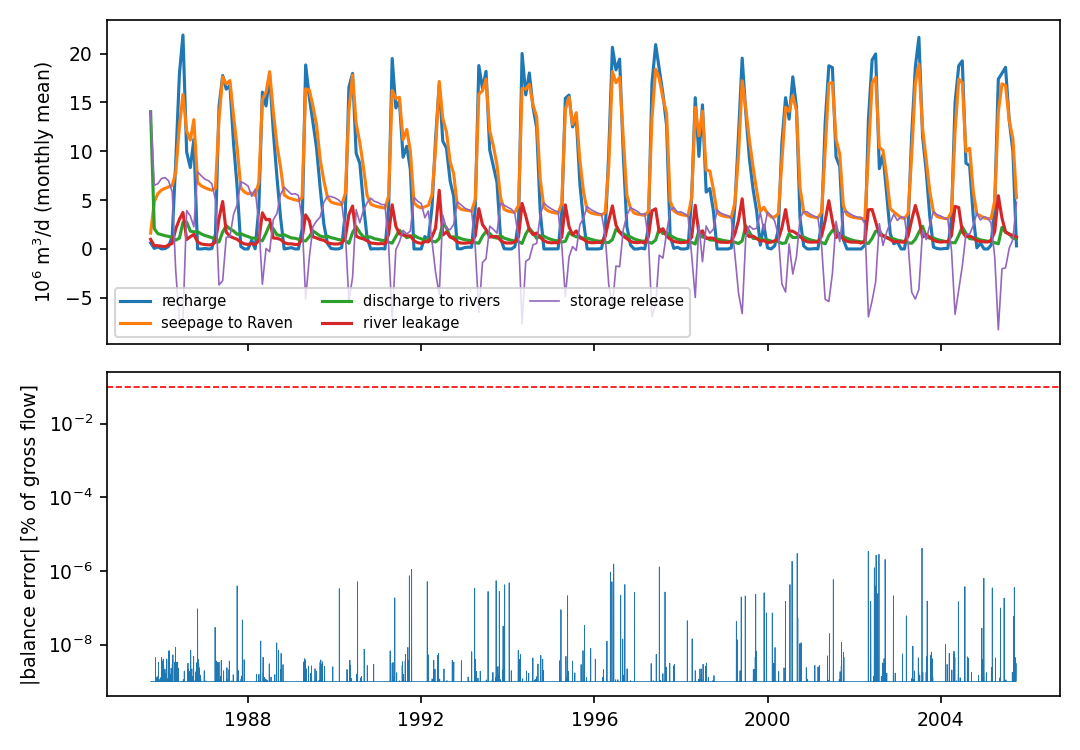
\includegraphics[width=\linewidth]{figures/fig_budget.png}
\caption{Groundwater budget of the 20-year Liard run (monthly means) and daily balance error; the dashed line is 0.1\%.}\label{fig:budget}\end{figure}
\begin{figure}[h]\centering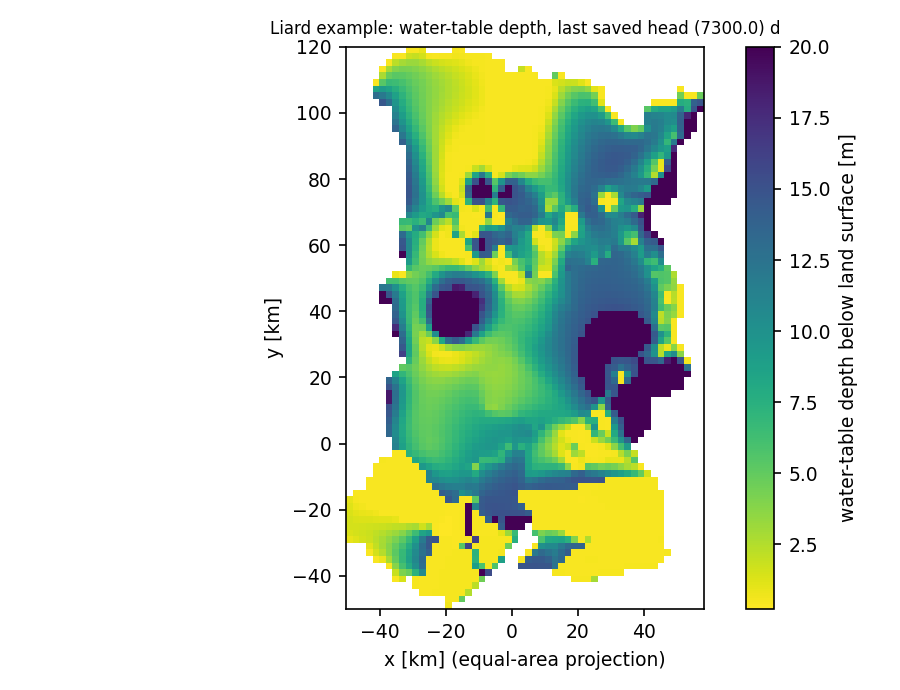
\includegraphics[width=0.72\linewidth]{figures/fig_wtdepth.png}
\caption{Depth to water at the last saved head.}\label{fig:wtdepth}\end{figure}
\begin{figure}[h]\centering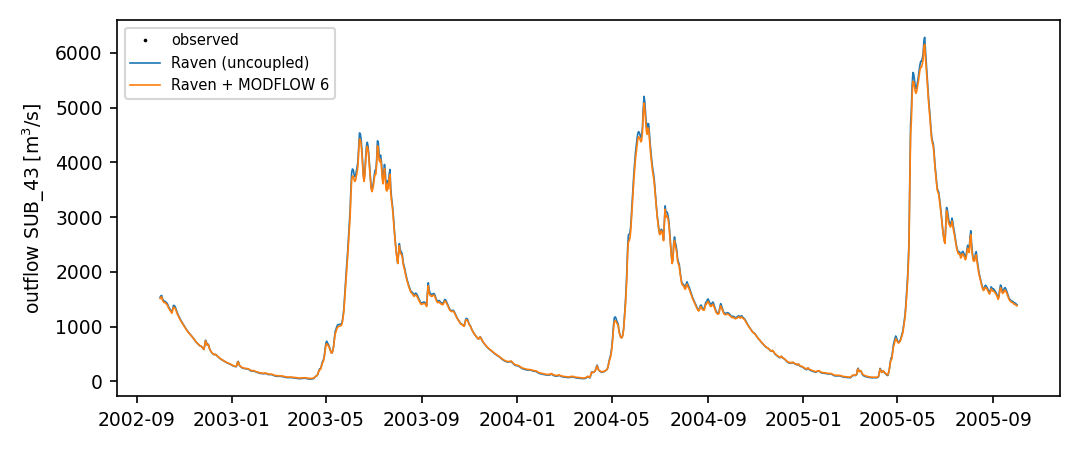
\includegraphics[width=\linewidth]{figures/fig_hydrograph.png}
\caption{Outflow of subbasin 43, 2003--2005, without and with groundwater (not recalibrated).}\label{fig:hydro}\end{figure}
Without recalibration and with stand-in geometry, the Nash--Sutcliffe efficiency at gauges 10BE004, 10BE005 and 10BE010
changes from 0.867, 0.835, 0.681 to 0.850, 0.821, 0.634. Recalibrating with flow and head data is the natural next step.

\section{Preparing the input data}
\subsection{HRU polygons}
Raven's HRUs usually come from a GIS overlay (for example BasinMaker): subbasins intersected with land-use, soil and terrain
classes. Export that polygon layer, keeping the HRU ID used in the \cmd{.rvh}:
\par\noindent\begin{minipage}{\linewidth}
\begin{lstlisting}
ogr2ogr -f GeoJSON -t_srs EPSG:4326 my_hrus.geojson my_hrus.shp
\end{lstlisting}
\end{minipage}\par\smallskip
(or, in QGIS, \emph{Export $\rightarrow$ Save Features As}, format GeoJSON, CRS EPSG:4326). Check that every HRU with an
\cmd{AQUIFER\_PROFILE} appears in the file; \cmd{GWModelSummary.txt} lists, per HRU, its polygon area, its area in the \cmd{.rvh}
and the fraction linked to active cells.
\subsection{Maps}
Convert the DEM and the bedrock (or aquifer base) surface to ESRI ASCII grids in longitude/latitude:
\par\noindent\begin{minipage}{\linewidth}
\begin{lstlisting}
gdalwarp -t_srs EPSG:4326 -tr 0.005 0.005 -r bilinear dem.tif dem_lonlat.tif
gdal_translate -of AAIGrid dem_lonlat.tif dem_lonlat.asc
\end{lstlisting}
\end{minipage}\par\smallskip
Use a raster resolution finer than the model cells (each model cell averages 25 samples). Both maps must use the same
vertical datum, as must well screens, monitoring wells, boundary heads and reservoir stages.
\subsection{River lines}
Any line layer of the river network in longitude/latitude. A field with the Raven subbasin ID is optional; without it, each
river piece is assigned to the subbasin of the HRU that dominates its grid cell.
\subsection{Aquifer information}
Layer thicknesses and materials come from borehole logs, geological maps or regional hydrogeological studies. Start with one or
two profiles and typical values (Section~\ref{ch:ownmodel}); refine only where data or calibration demand it.

\section{Choosing a grid for the Liard model}\label{sec:liardgrids}
The Liard model was run for two years on each grid option (Table~\ref{tab:liardgrids}); every run keeps the water accounts
exact (MODFLOW residual about $10^{-11}$, no failed step, Raven's balance unchanged).
\begin{table}[!htbp]\centering
\caption{The Liard model (2 years) on each grid: active cells, run time on one core, Nash--Sutcliffe efficiency at 10BE004 /
10BE005 / 10BE010, mean seepage to Raven and mean net aquifer discharge to rivers [million m$^3$/d].}\label{tab:liardgrids}
\begin{tabular}{lrrcrr}\toprule\hdr
Grid & Cells & Time [s] & NSE & Seepage & Rivers\\\midrule
Regular 2 km (default) & 8\,840 & 40 & 0.728 / 0.861 / 0.635 & 9.48 & 0.82\\
Regular, rotated 20\textdegree, 1 km along rivers & 35\,058 & 220 & 0.726 / 0.861 / 0.638 & 9.92 & 0.66\\
Quadtree 2 km, 500 m along rivers & 16\,276 & 108 & 0.719 / 0.858 / 0.611 & 9.49 & 0.01\\
HRU mesh 2 km, 1 km along rivers & 14\,610 & 100 & 0.717 / 0.859 / 0.627 & 9.94 & 0.35\\
Regular 2 km, layers by elevation & 8\,840 & 41 & 0.666 / 0.859 / 0.606 & 4.11 & 0.49\\
\bottomrule\end{tabular}
\par\smallskip\footnotesize Final code with MODFLOW 6.8.1 (\cmd{tests/liard\_grids.py}); run times on one core of the test machine.
\end{table}
Streamflow hardly changes: total seepage is nearly the same on every grid and the river exchange is a small part of the
flow at the gauges. The net river exchange, however, depends on the size of the river cells --- 0.82 million m$^3$/d with
2 km cells, 0.01 with 500 m cells --- for two reasons: the channel bed is placed at the lowest DEM value along the river in
each cell, which is lower in larger cells, and the head of a large cell averages the aquifer over a wider area around the
river. Calibrate the riverbed parameters (\cmd{RIVERBED\_K}, \cmd{:RiverBedDepth}) on the grid that will be used, and
compare models only at the same river-cell size. Connecting layers by elevation halves the seepage here, because water in
the upland till can now flow directly into the valley gravel where the two lie at the same elevation --- a different
conceptual model rather than a refinement. A regular grid refined to 1 km along rivers has more than twice the cells of a
quadtree with 500 m river cells, because its refinement spans whole rows and columns.

\section{Setting up your own model}\label{ch:ownmodel}
\subsection{Checklist}
\begin{enumerate}
\item \textbf{HRU polygons.} Export the HRU polygons from your GIS or BasinMaker as GeoJSON in longitude/latitude
(EPSG:4326), with a field holding the HRU ID used in the \cmd{.rvh} file.
\item \textbf{Maps.} A DEM and a bedrock (or aquifer-base) elevation map as ESRI ASCII grids in longitude/latitude, in the same
vertical datum. River lines as GeoJSON.
\item \textbf{Profiles.} Group your HRUs by the aquifer beneath them and write one profile per group; set
\cmd{AQUIFER\_PROFILE} in the \cmd{.rvh}.
\item \textbf{Recharge.} Decide which Raven flux is recharge (usually percolation from the deepest soil store) and send it
to \cmd{GROUNDWATER} for coupled HRUs only. Remove or restrict any process that drains \cmd{GROUNDWATER} there, and any
conceptual baseflow that would double-count groundwater.
\item \textbf{Grid size.} Choose $\Delta$ so that the smallest features you care about span a few cells, but the number of
active cells stays manageable (a few thousand to a few hundred thousand per layer).
\item \textbf{Start.} Use \cmd{:GWInitialization STEADY\_STATE} with the long-term average recharge, or a warm-up period.
\item \textbf{Check.} Read \cmd{GWModelSummary.txt} and run \cmd{tools\_audit.py}.
\item \textbf{Calibrate.} Use streamflow and monitoring-well heads (Section~\ref{ch:calib}).
\end{enumerate}

\section{Typical parameter values}
Typical values for aquifer materials are listed in Section~\ref{app:materials}, and typical ranges for every aquifer class
and profile parameter in Sections~\ref{app:class} and~\ref{app:profile}.

\subsection{How much of the water balance should groundwater take?}
In a coupled HRU, Raven's conceptual baseflow from deep stores is replaced by MODFLOW. Check after a first run that the
long-term baseflow (seepage plus aquifer discharge to rivers) is plausible, and that the aquifer is not steadily filling or
emptying (storage release near zero on average once spin-up is over).

\section{Calibration}\label{ch:calib}
Aquifer class and profile parameters are ordinary entries in the \cmd{.rvp} file, so they can be calibrated with Ostrich
exactly like soil parameters: make a template of the \cmd{.rvp} with parameter names in place of values.
\par\noindent\begin{minipage}{\linewidth}
\begin{lstlisting}
  GRAVEL,      par_K_gravel, 5.0,  1.0E-5, par_Sy_gravel, 0.30
  UPLAND_TILL, par_K_till,   0.02, 1.0E-4, 0.08,          0.30
\end{lstlisting}
\end{minipage}\par\smallskip
Monitoring-well heads (\cmd{:ObservationData GW\_HEAD}) are scored in \cmd{Diagnostics.csv} next to streamflow, so an
objective can combine both. Calibrate conductivities on a logarithmic scale. \cmd{docs/ostrich\_example/} contains an
\cmd{ostIn.txt} using DDS \cite{tolson2007dds}, the template and run scripts. Because the linkage is cached, repeated runs
skip the geometry work.

\subsection{A synthetic test}
Groundwater under subbasin 52 only (545 active columns), 2 years, 7 s per run. Heads from a run with known parameters, plus
2 cm of random noise, at four monitoring wells were the observations. The search started from values 2.5 to 10 times off.
\begin{table}[!htbp]\centering
\caption{Synthetic calibration: the parameters used to make the ``observations'', the starting values, and the values DDS recovered.}\label{tab:synthcal}
\begin{tabular}{lrrrr}\toprule\hdr
Parameter & True & Start & After 150 runs & Error\\\midrule
Gravel $K$ [m/d] & 50 & 5 & 47.7 & $-4.6$\%\\
Gravel $S_y$ & 0.25 & 0.10 & 0.239 & $-4.5$\%\\
Upland-till $K$ [m/d] & 0.2 & 2.0 & 0.149 & $-25$\%\\\bottomrule
\end{tabular}\end{table}
Table~\ref{tab:synthcal} shows the result. The objective (sum of RMSE over the four wells) fell from 14.4 m to 0.17 m (it is 0.08 m at the true values, so more runs
would refine it further; Figure~\ref{fig:calib}). The upland-till conductivity is the hardest to identify because the
upland heads respond weakly to it.
\begin{figure}[h]\centering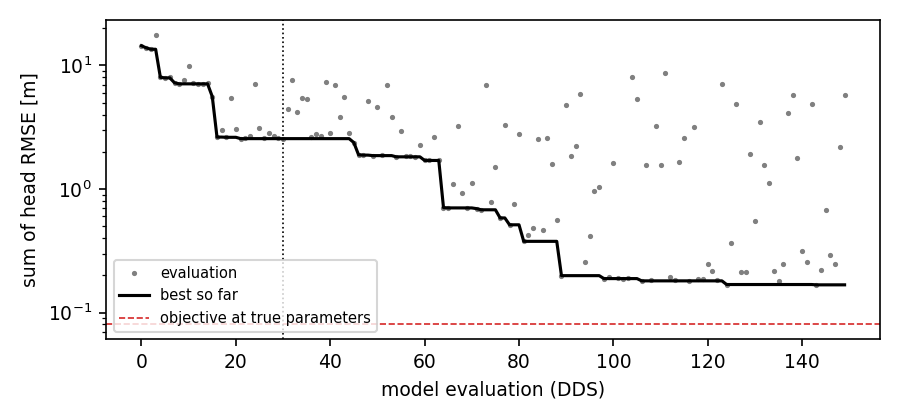
\includegraphics[width=0.8\linewidth]{figures/fig_calibration.png}
\caption{Synthetic calibration: objective against model runs.}\label{fig:calib}\end{figure}

\section{The Ostrich input file, line by line}
\begin{lstlisting}
ProgramType         DDS             # search algorithm (dynamically dimensioned search)
ObjectiveFunction   GCOP            # general constrained optimization
ModelExecutable     ./Ost-Raven.sh  # script that runs Raven in ./model
BeginFilePairs
  Liard.rvp.tpl ; model/Liard.rvp   # template -> model file with values filled in
EndFilePairs
BeginParams                         # name, start, lower, upper, transformations
  par_K_gravel   5.0  1.0  500.0  none log10 none
  par_Sy_gravel  0.10 0.05 0.35   none none  none
  par_K_till     2.0  0.01 5.0    none log10 none
EndParams
BeginResponseVars                   # values read from Diagnostics.csv
  RMSE1  model/output/Diagnostics.csv ; OST_NULL 1 5 ','
  ...
EndResponseVars
BeginTiedRespVars                   # objective = sum of the RMSEs
  SUM_RMSE 4 RMSE1 RMSE2 RMSE3 RMSE4 wsum 1.0 1.0 1.0 1.0
EndTiedRespVars
BeginGCOP
  CostFunction SUM_RMSE
EndGCOP
BeginDDSAlg
  MaxIterations 150
EndDDSAlg
\end{lstlisting}
Check the row and column of each response in your own \cmd{Diagnostics.csv}; they depend on the order of observations and on
\cmd{:EvaluationMetrics}. To combine heads and streamflow, add NSE or KGE responses of the hydrographs with suitable weights.

\section{Troubleshooting}\label{ch:trouble}
\begin{table}[!htbp]\centering
\caption{Messages and symptoms, with their causes and remedies.}
\begin{tabular}{P{0.36\linewidth}P{0.588\linewidth}}\toprule\hdr
Message or symptom & Cause and remedy\\\midrule
``cannot load MODFLOW 6 library'' & run \cmd{python tools/get\_mf6.py} in the source folder, or set \cmd{:MF6Library} or \cmd{RAVEN\_MF6\_LIB} to the full path of \cmd{libmf6}; the message lists the places searched\\
Raven stops during initialization without a Raven message & MODFLOW rejected its input; read \cmd{<output>/mf6/mfsim.lst}\\
``HRU \dots\ has an AQUIFER\_PROFILE but no polygon'' & HRU IDs in the GeoJSON do not match the \cmd{.rvh}; check the ID field name\\
``does not overlap any active groundwater cell'' & the HRU is too small for the grid or sits where bedrock is at the surface; reduce \cmd{:GridCellSize} or \cmd{:MinCellCoverage}, or check the bedrock map\\
``polygon area \dots\ differs from .rvh AREA'' & information only; volumes are always consistent\\
``process \dots\ removes water from GROUNDWATER'' & a Raven process drains \cmd{GROUNDWATER} in a coupled HRU; restrict it with \cmd{:-->Conditional}\\
``process \dots\ sends water to GROUNDWATER in HRU \dots\ which has no AQUIFER\_PROFILE'' & that water would leave the model; restrict the process\\
``MODFLOW 6 did not converge'' & start from a steady state or realistic heads; raise \cmd{:SolverMax\allowbreak OuterIterations}; increase \cmd{SEEPAGE\_SMOOTHING\_DEPTH}; check for extreme parameter contrasts\\
Well rate is zero (``no :WellRate time series'') & the \cmd{:WellRate} block is missing, or its ID does not match an ID in \cmd{:Wells}\\
``reservoir \dots\ has no :SeepageParameters'' / ``no coupled lake HRU'' & add \cmd{:SeepageParameters}; give the lake HRU an \cmd{AQUIFER\_PROFILE}\\
``running more time steps than the MODFLOW 6 simulation holds'' & \cmd{:Duration} or \cmd{:TimeStep} is inconsistent; rerun\\
Water table far above the land surface & \cmd{SEEPAGE\_LEAKANCE} too small, or $K$ too low for the recharge\\
Aquifer steadily emptying for years & initial heads too high; use a steady-state start or a longer spin-up\\\bottomrule
\end{tabular}
\end{table}

\section{Frequently asked questions}
\paragraph{Do I need MODFLOW experience?} No. Raven writes and runs the MODFLOW model. It helps to know the concepts of
Chapter~\ref{ch:c2}; the generated files can be inspected by anyone who knows MODFLOW.
\paragraph{Can only part of my watershed have groundwater?} Yes. Only HRUs with an \cmd{AQUIFER\_PROFILE} are coupled; all
others run exactly as before.
\paragraph{Can two aquifer systems exchange water?} Yes, when their cells touch: lateral flow between neighbouring profiles and
leakage between layers are computed by MODFLOW like any other flow.
\paragraph{What happens where the water table reaches the surface?} The seepage drains return the water to Raven, where it
follows Raven's processes (for example baseflow to the river).
\paragraph{Can the aquifer take more water than a river carries?} No: the supply limit caps each river cell's largest
possible loss at its share of the reach's flow.
\paragraph{How do I restart a long run?} Use \cmd{solution.rvc} of the finished run as the \cmd{.rvc} of the next, with
\cmd{:StartDate} set to the end of the first run.
\paragraph{How fine should the grid be?} Fine enough that valleys and well spacings span two or three cells
(Section~\ref{ch:grid}). Coarser grids run faster.
\paragraph{How long a spin-up do I need?} Start from a steady state with the long-term mean recharge, then check that
\emph{storage release} in \cmd{GWBudget.csv} averages near zero over the first years; large, slow aquifers may need decades.
\paragraph{Can I see the head everywhere, not only at wells?} Yes: \cmd{mf6/gwf.hds} (MODFLOW binary, readable with FloPy)
every \cmd{:HeadSaveFrequency} steps, or \cmd{GWHeads.nc} with \cmd{:WriteNetCDFHeads}.
\paragraph{Does the coupling change results for my other subbasins?} Only through the rivers: groundwater discharge or losses
in coupled subbasins change the flow passed downstream.
\paragraph{Can I use it in an ensemble or with Ostrich?} Yes; each ensemble member rebuilds and restarts MODFLOW, and aquifer
parameters are ordinary \cmd{.rvp} values.
\paragraph{What if MODFLOW stops the program?} Read \cmd{<output>/mf6/mfsim.lst}; it names the file and value MODFLOW rejected.

\chapter{Verification and code audit}\label{ch:c8}\label{ch:verification}
This chapter reports how the coupling was tested and what was found. Nine complementary approaches were used
(Table~\ref{tab:vapproach}); every problem they uncovered is listed, with its correction, in Section~\ref{sec:findings}.

\begin{plain}
Before anyone relies on a model, it must be shown to be right. The coupling was tested in several independent ways:
automatic checks that no water is created or lost, comparisons with exact textbook solutions, comparisons with independent
software, hundreds of random test set-ups, and a line-by-line review of the code. Every problem found along the way is
listed at the end of the chapter with how it was fixed.
\end{plain}

\begin{table}[!htbp]\centering
\caption{Verification approaches.}\label{tab:vapproach}
\begin{tabularx}{\linewidth}{P{0.27\linewidth}Y P{0.13\linewidth}}\toprule\hdr
Approach & What it shows & Section\\\midrule
Regression against Raven 4.15 & models without groundwater give identical results & \ref{sec:regression}\\
Automated audit of every run & exact water accounting on both sides; MODFLOW's balance & \ref{sec:audit}\\
Behaviour tests & pumping, drying, restarts, ensembles and every exchange behave as expected & \ref{sec:behaviour}\\
Grid types & geometry, format cross-checks, analytical solution, restarts and randomized tests for every grid & \ref{sec:vgrids}\\
Existing model & projections, units, round trip, overlap weights, restarts, safeguards, randomized tests & \ref{sec:vexisting}\\
Independent checks & geometry against standard libraries; flows against MODFLOW's own budget; grid and time-step invariance; faulty input & \ref{sec:independent}\\
Randomized testing & hundreds of random set-ups combining every option & \ref{sec:fuzz}\\
Release audit & five-step audit of the final package; checks of every MODFLOW input file and of faulty input without MODFLOW; one command repeats every test & \ref{sec:relaudit}\\
Code audit & line-by-line review, compiler, static analysis, memory and undefined-behaviour sanitizers & \ref{sec:codeaudit}\\\bottomrule
\end{tabularx}
\end{table}

\section{Models without groundwater are unchanged}\label{sec:regression}
The coupling was developed on Raven~4.1.1 and then carried over to Raven~4.15 (Section~\ref{sec:port}). Models without
groundwater were run with the unmodified Raven~4.15 and with the coupled code, both built with NetCDF:
\begin{itemize}
\item the Liard model: all outputs identical byte for byte;
\item the benchmark models distributed with Raven (\cmd{benchmarking/\_InputFiles}): the eleven that run give identical
      outputs, except that Lake of the Woods, whose reservoir in basin~44 dries out on 45 days, books less evaporation on
      those days (the correction of Section~\ref{sec:findings}). Its hydrographs and reservoir stages are identical; its
      cumulative balance error falls from 5.44 to 4.97~mm, and its \cmd{solution.rvc} carries the reservoir stages with 12
      digits. The other fourteen benchmark set-ups stop with the same input error in both builds (a missing \cmd{.rvt} file,
      wilting point above field capacity), as they do in the unmodified Raven~4.15.
\end{itemize}
The corrections made to Raven itself (Section~\ref{sec:findings}) affect only ensembles, reservoirs with absolute stages or
that dry out, restart files, constituent observations and the \cmd{:rvg\_Filename} command.

\subsection{Carrying the coupling over to Raven 4.15}\label{sec:port}
Between 4.1.1 and 4.15, 157 of Raven's source files changed. A three-way merge (Raven~4.1.1, the coupling, Raven~4.15) left 26
overlapping edits in 22 files; each was resolved by hand:
\begin{itemize}
\item copyright headers (13): the 4.15 year kept, with the line naming the modification;
\item observation diagnostics: 4.15's new rule for observations without a subbasin kept, with \cmd{GW\_HEAD} handled
      first (its location is a monitoring well);
\item initial conditions: the new groundwater commands of the \cmd{.rvc} file beside 4.15's new management commands;
\item ensembles: 4.15's \cmd{RebootTimeVariables} (which resets the balance arrays between members) kept beside the
      restoring of routing memory and reservoir states; the history setters now take the time step, as in 4.15;
\item reservoirs: 4.15 replaced the data-assimilation scale factor by an additive adjustment; the reservoir snapshot for
      ensemble members and the 12-digit \cmd{solution.rvc} values follow that change;
\item BMI: 4.15 had already corrected the index in \cmd{SetValueAtIndices} in the same way, so its version was taken;
\item the Visual Studio project files were rebuilt from 4.15's, with the MODFLOW-USG files replaced by the new ones.
\end{itemize}
Raven~4.15 prints its closing message (\emph{Exiting Gracefully}) to the error stream; the test scripts read both streams.
The whole test suite was then repeated on the ported code with MODFLOW~6.8.1 and~6.6.3 (Section~\ref{sec:relaudit}).

\section{Automated audit of every run}\label{sec:audit}
The tool \cmd{tools\_audit.py}, shipped with the example, checks any output folder for:
\begin{enumerate}
\item \textbf{recharge:} $\left(\sum V^{\mathrm{Raven}}-\sum V^{\mathrm{MF6}}-\Delta S^{\mathrm{delay}}-\sum V^{\mathrm{CHD}}\right)/\sum V^{\mathrm{Raven}}$;
\item \textbf{MODFLOW's balance:} cumulative imbalance relative to the gross flow, and the worst single step;
\item \textbf{convergence:} steps that failed to converge;
\item \textbf{seepage, rivers and surface stores:} the volume applied to Raven against MODFLOW's flow, including carried river losses;
\item \textbf{reservoirs:} the seepage sent to MODFLOW each step against the volume that left the lake the step before, and
      the volume MODFLOW took against the volume sent;
\item \textbf{Raven's balance:} the largest mass-balance error in \cmd{Watershed\allowbreak Storage.csv};
\item \textbf{outputs:} finite heads, contiguous end-of-step dates, a $t=0$ row for monitoring wells.
\end{enumerate}
Table~\ref{tab:audit} gives the results. They were first obtained before the release audit (Section~\ref{sec:relaudit}); with
the final code the 20-year Liard run gives outputs identical to those runs, and the reservoir and ensemble runs were repeated
(Section~\ref{sec:behaviour}).

\begin{table}[!htbp]\centering
\caption{Automated audit (\cmd{tools\_audit.py}); the reservoir and ensemble rows are from the final code's repeat (\cmd{tests/behaviour\_check.py}), the 20-year Liard run is identical with the final code. Relative errors are shares of the water moved. In every run the seepage returned to Raven equals MODFLOW\textquotesingle s seepage exactly, the surface-store bookkeeping is exact, no river loss is carried at the end and the output dates are contiguous. The one failed step is the rewetting day of the deliberately extreme drying test (Section~\ref{sec:behaviour}).}\label{tab:audit}
\footnotesize\setlength{\tabcolsep}{2.8pt}\begin{tabular}{lrrrrrrr}\toprule\hdr
Run & Steps & Recharge & \shortstack[r]{MODFLOW\\residual} & \shortstack[r]{Worst\\step [\%]} & \shortstack[r]{Failed\\steps} & River & \shortstack[r]{Raven\\balance [mm]}\\\midrule
20-year Liard & 7\,305 & 0 & $-1.0\times10^{-10}$ & $4.2\times10^{-6}$ & 0 & $1.1\times10^{-12}$ & 0.52\\
Pumping & 1\,826 & 0 & $-1.6\times10^{-10}$ & $7.1\times10^{-6}$ & 0 & $-9.6\times10^{-12}$ & 0.52\\
Fixed head, delay & 730 & $-3.2\times10^{-11}$ & $-3.9\times10^{-10}$ & $5.1\times10^{-6}$ & 0 & $7.7\times10^{-12}$ & 0.52\\
Restart & 365 & $-1.7\times10^{-11}$ & $-1.9\times10^{-10}$ & $3.2\times10^{-6}$ & 0 & $2.1\times10^{-11}$ & 0.06\\
Ensemble & 731 & 0 & $-1.7\times10^{-11}$ & $1.6\times10^{-7}$ & 0 & $9.5\times10^{-12}$ & 0.52\\
Wetlands & 730 & 0 & $-1.1\times10^{-10}$ & $1.5\times10^{-6}$ & 0 & $2.2\times10^{-11}$ & 0.52\\
Reservoir & 731 & 0 & $-1.7\times10^{-11}$ & $1.6\times10^{-7}$ & 0 & $9.5\times10^{-12}$ & 0.52\\
Soil-less HRUs & 365 & 0 & $-4.5\times10^{-11}$ & $7.4\times10^{-7}$ & 0 & $-1.2\times10^{-12}$ & 0.52\\
Drying (extreme) & 1\,826 & 0 & $-3.1\times10^{-4}$ & 43.2 & 1 & $8.1\times10^{-12}$ & 0.52\\
\bottomrule\end{tabular}\end{table}


\section{Behaviour tests}\label{sec:behaviour}
\begin{table}[!htbp]\centering
\caption{Behaviour tests.}\label{tab:behaviour}
\begin{tabularx}{\linewidth}{P{0.19\linewidth}P{0.27\linewidth}Y}\toprule\hdr
Test & Set-up & Result\\\midrule
Full Liard model & 20 years, 85 coupled HRUs, 3\,252 active columns & recharge exact; MODFLOW residual $10^{-10}$; no failed step; Raven balance 0.52 mm\\
Pumping & 100\,000 m$^3$/d well, 5 years & 93\% delivered; seasonal drawdown 0.8--8 m in the pumped cell, none 12 km away; 91--98\% of the water captured from rivers (Figure~\ref{fig:pumping})\\
Monitoring wells & synthetic heads with 5 cm noise & RMSE 4.9 cm; NSE 0.991--0.9997\\
Fixed-head lake & 9 cells & heads held exactly; recharge on them redistributed\\
Restart & 1 + 1 years against 2 years & flows within $6\times10^{-6}$ (Figure~\ref{fig:hotstart})\\
Ensembles & 2 Monte Carlo members, every option on & members identical to each other and to a single run\\
Drying and rewetting & valley aquifer starting dry & 26 wet areas merge into 2 and split with the seasons (Figure~\ref{fig:conn}); one rewetting step of 1\,826 does not converge and is flagged\\
Wetlands and lakes & 1\,903 exchange cells & water removed from Raven equals MODFLOW's leakage exactly\\
Reservoir & 50 km$^2$ lake on a coupled HRU & seepage delivered each day equals Raven's seepage of the day before\\
Soil-less HRUs & glacier HRUs coupled & seepage goes to surface water; balance unchanged\\
Other features & \cmd{:rvg\_Filename}, NetCDF, linkage cache, calibration & file found; NetCDF equals the binary heads within $10^{-4}$ m; cached run identical; DDS recovers gravel $K$ and $S_y$ within 5\%\\\bottomrule
\end{tabularx}
\end{table}

The tests on the regular-grid Liard model were first run before the release audit. With the final code (MODFLOW 6.8.1) the
20-year run gives outputs identical to that earlier run --- budget, heads, hydrographs, storage and restart file --- so these
results and the figures drawn from them stand. The two rows the audit's corrections could change were repeated with the final
code (\cmd{tests/behaviour\_check.py}): a 50~km$^2$ lake with seepage on the largest coupled HRU of subbasin~52, with a
pumping well, for two years --- the seepage MODFLOW received each day equals the volume that left the lake the day before
(difference 0), all of it delivered, MODFLOW residual $1.7\times10^{-11}$; and the same set-up as a two-member ensemble ---
both members identical to the single run (difference 0).

\begin{figure}[!htbp]\centering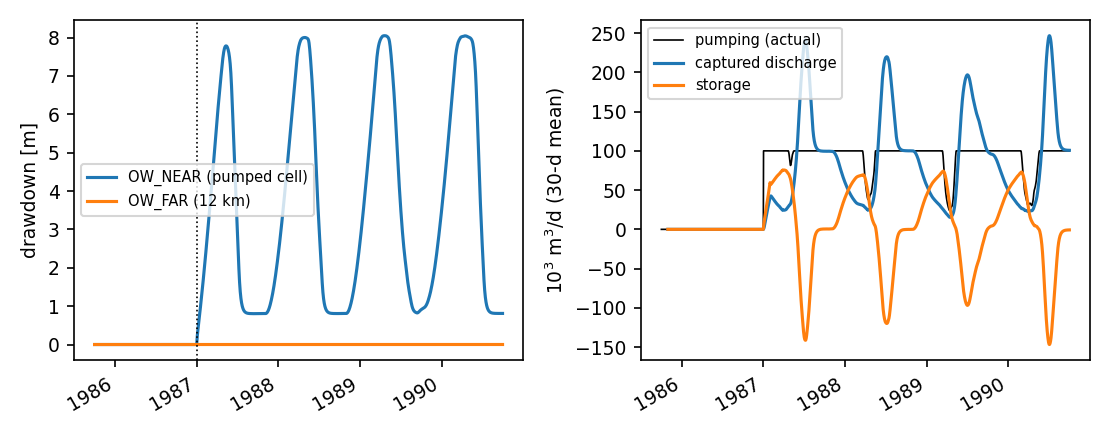
\includegraphics[width=\linewidth]{figures/fig_pumping.png}
\caption{Pumping test: drawdown at the monitoring wells (left) and where the pumped water comes from (right).}\label{fig:pumping}\end{figure}
\begin{figure}[!htbp]\centering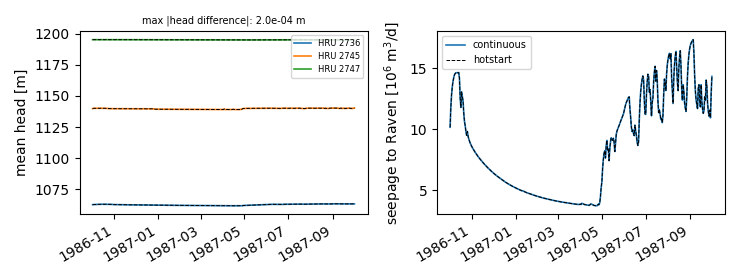
\includegraphics[width=\linewidth]{figures/fig_hotstart.png}
\caption{Restart: the second year of a continuous run (solid) and of a run restarted from \cmd{solution.rvc} (dashed).}\label{fig:hotstart}\end{figure}
\begin{figure}[!htbp]\centering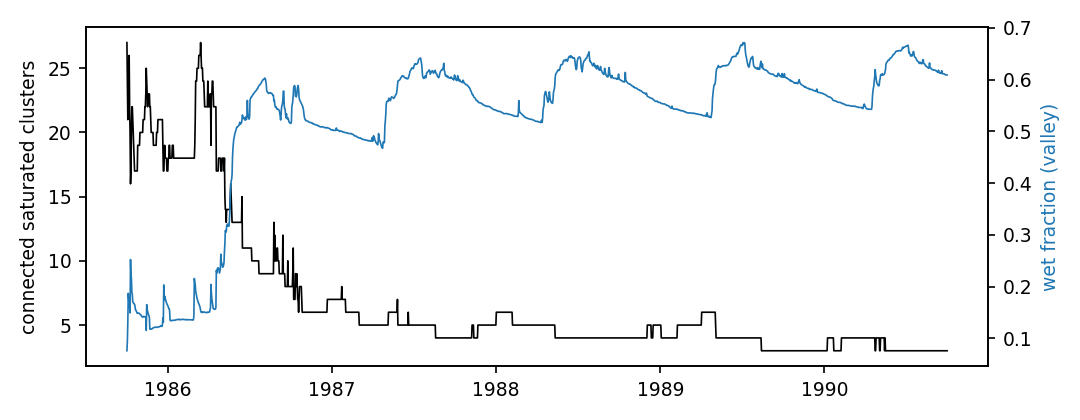
\includegraphics[width=0.9\linewidth]{figures/fig_connectivity.png}
\caption{Drying and rewetting: number of separate wet areas in the top layer (black) and wet fraction of the valley aquifer (blue).}\label{fig:conn}\end{figure}

\section{Independent checks}\label{sec:independent}
\subsection{Geometry against standard libraries}
The geometry functions were compiled into a stand-alone test and compared with widely used libraries (Table~\ref{tab:geom}).
\begin{table}[!htbp]\centering
\caption{Geometry functions against independent libraries.}\label{tab:geom}
\begin{tabularx}{\linewidth}{Y P{0.22\linewidth}P{0.2\linewidth}}\toprule\hdr
Function & Reference & Largest difference\\\midrule
Polygon clipping and area (400 random, mostly concave polygons) & shapely & $1.3\times10^{-10}$\\
Equal-area projection (300 points over the Liard region) & pyproj (same sphere) & $5\times10^{-7}$ m\\
Projection round trip & -- & exact\\
Bilinear raster sampling with a no-data cell (200 points) & independent code & $4\times10^{-7}$\\
GeoJSON and ASCII-grid variants (3-D coordinates, string IDs, holes, cell-centre headers, \dots) & shapely, reference values & read correctly\\\bottomrule
\end{tabularx}
\end{table}

\subsection{Exchanged flows against MODFLOW's own budget}
MODFLOW writes its own volume budget in its list file. For runs covering every package, every flow the coupling exchanged
was compared with MODFLOW's figure for the same step (Table~\ref{tab:listcheck}); the differences are at the printing
precision of the list file.
\begin{table}[!htbp]\centering
\caption{Coupler flows against MODFLOW's list-file budget.}\label{tab:listcheck}
\begin{tabularx}{\linewidth}{P{0.25\linewidth}Y P{0.2\linewidth}}\toprule\hdr
Run & Packages compared & Largest difference\\\midrule
20-year Liard & recharge, drains, rivers, storage & $6.2\times10^{-7}$\\
Pumping and boundaries & + wells, general-head boundaries & $6.9\times10^{-7}$\\
Fixed head and delay & + fixed heads & $6.1\times10^{-8}$\\
Wetland exchange & + store exchange & $1.1\times10^{-7}$\\
Reservoir & + reservoir seepage & $2.6\times10^{-7}$\\
Drying & + water-table ET & $4.1\times10^{-8}$\\\bottomrule
\end{tabularx}
\end{table}

\subsection{Grid size and time step}
The accounts stay exact for any cell size and time step (Table~\ref{tab:invariance}; subbasin 52, one year). These runs used
the earlier head tolerance of 0.01 m; the 0.47\% step on 4 km cells is what led to the present default of 0.00001 m.
\begin{table}[!htbp]\centering
\caption{Invariance to cell size and time step.}\label{tab:invariance}
\begin{tabular}{lrlrr}\toprule\hdr
Set-up & Active columns & Recharge & Worst step & Raven balance\\\midrule
1 km cells & 2\,147 & exact & 0.029\% & 0.456 mm\\
2 km cells & 545 & exact & 0.092\% & 0.456 mm\\
4 km cells & 142 & exact & 0.47\% & 0.456 mm\\
4 km cells, tighter tolerance & 142 & exact & 0.002\% & 0.456 mm\\
2 km cells, half-day steps & 545 & exact & 0.059\% & 0.219 mm\\\bottomrule
\end{tabular}
\end{table}

\subsection{Faulty input}
Thirty-nine faulty or unusual set-ups were run. Every error stops the run with a message that names the problem --- no crash
--- and every tolerated case runs (Table~\ref{tab:faulty}).
\begin{table}[!htbp]\centering
\caption{Response to faulty or unusual input.}\label{tab:faulty}
\begin{tabularx}{\linewidth}{Y P{0.4\linewidth}}\toprule\hdr
Input & Response\\\midrule
Missing HRU file or ID field; unknown profile or class; malformed class row & stops; names the file, field, profile or row\\
Aquiclude as top layer; zero layer thickness; value out of range ($K\le0$, $S_y>1$, negative delay, \dots) & stops; names the parameter\\
Process draining \cmd{GROUNDWATER} in a coupled HRU; no process feeding it & stops; names the process and HRU\\
Wrong library path; missing raster; well outside the model & stops; names the path, file or well\\
Duplicate IDs or names; two exchanges on one store; boundary without \cmd{HEAD} & stops; names the item\\
Malformed groundwater command in \cmd{.rvg}, \cmd{.rvt} or \cmd{.rvc} & stops; names the command\\
Hotstart heads for a different grid; cells larger than the HRUs & stops; explains the mismatch\\
Monitoring well outside the model; unknown \cmd{.rvg} command & runs with a warning\\
\cmd{TO\_BEDROCK} in a middle layer; no DEM or bedrock map; coupling switched off & runs as documented\\\bottomrule
\end{tabularx}
\end{table}

\section{Randomized testing}\label{sec:fuzz}
A test driver builds random but valid set-ups of the subbasin-52 model, drawing every option at random: cell size
(1--3 km), minimum coverage, one-day or half-day steps, conductivities, initial depth, seepage leakance and smoothing,
water-table ET, recharge delay, steady-state start, wetland exchange, 0--2 pumping wells, monitoring wells, a general-head
boundary, a fixed-head area and a coupled reservoir. Every run is checked independently of the audit tool: exact recharge,
seepage, river, store and reservoir identities; MODFLOW's balance (every converged step below 0.1\%, cumulative below
$10^{-4}$); Raven's balance below 1 mm; agreement with MODFLOW's list file; and, for about a third of the set-ups, a restart
that must reproduce the continuous run (every flow within $10^{-4}$ of its largest value in the run).

Rounds of review and randomized testing were repeated until a complete round found no model error: nine rounds and 480 random
set-ups in all. The final code, with MODFLOW 6.8.1, passes the rounds that \cmd{tests/run\_all.py} repeats: 72 of 72 set-ups
over every grid type and 24 of 24 with a reservoir and lake refinement (Section~\ref{sec:vgrids}).

\section{Grid types}\label{sec:vgrids}
\begin{plain}
Every kind of grid was checked in four ways: its cells cover the area exactly with no gaps or overlaps; two different ways of
handing the same cells to MODFLOW give the same answer; the answer matches an exact textbook solution and gets closer to it
as the cells get smaller; and a restarted run matches a continuous one. Existing models are not affected by the new options.
\end{plain}
Every grid option was verified the same way as the default grid, plus four checks specific to grids.

\paragraph{Existing models are unchanged.} With the default grid every output of the coupled Liard model (budget,
hydrographs, storage, HRU state, connectivity) and the generated MODFLOW files are identical byte for byte to those of the
code before the grid options were added.

\paragraph{Geometry of the grids.} A stand-alone test checks every generator: cells tile the domain exactly (area sums
equal to $10^{-15}$), neighbours are symmetric, each cell's perimeter equals its shared faces plus the domain edge, Voronoi
connections are exactly orthogonal, quadtree neighbours differ by one level at most, clipping handles concave cells and
lattices of cocircular seeds, and grids survive the linkage cache bit for bit.

\paragraph{Two formats, one answer.} The quadtree cells were run once as DISV (MODFLOW computes the geometry) and once
imported as DISU (the coupler computes connection lengths, face widths and directions): all flows agree to $6\times10^{-7}$ and
water tables to 0.3 mm. A regular grid written as DISU gives heads identical to DIS. Solving the coupler's DISU equations
independently in Python reproduces MODFLOW's heads to $3\times10^{-8}$ m.

\paragraph{Analytical solution.} A textbook case has an exact answer to compare with: a single well pumping from an aquifer
whose water level is held fixed all around, far away (the \emph{Thiem} solution). Close to the well the water level falls in
a known way with distance. A well pumping 5\,000 m$^3$/d from a confined aquifer ($T=500$ m$^2$/d) inside a
20 km square with fixed heads on its edge should give the Thiem profile $h=A+\frac{Q}{2\pi T}\ln r$. The slope fitted to
all cells between four cell sizes and 3 km from the well is compared with $Q/(2\pi T)$ in Table~\ref{tab:thiem}: every grid
converges to the analytical value as its cells shrink, and the solutions are symmetric around the well (slopes in the four
directions within 0.6\%).

\begin{table}[!htbp]\centering
\caption{Thiem test: error of the fitted slope $\partial h/\partial\ln r$.}\label{tab:thiem}
\begin{tabular}{lrrr}\toprule\hdr
Grid & Coarse & Medium & Fine\\\midrule
Regular, 500 / 250 / 125 m & +0.60\% & +0.04\% & +0.01\%\\
Regular 250 m, rotated 17\textdegree & & +0.03\% & \\
Regular 1 km refined to 125 m at the wells & & +1.01\% & \\
Quadtree, base 1\,000 / 500 / 250 m, 62.5 m at the wells & +0.80\% & +0.59\% & +0.26\%\\
Imported cells (the 250 m quadtree) & & & +0.25\%\\
HRU mesh, 500 / 250 m (250 m with XT3D) & +0.57\% & +0.29\% & $-$0.06\%\\\bottomrule
\end{tabular}
\par\smallskip\footnotesize Final code with MODFLOW 6.8.1 (\cmd{tests/thiem}); every run audited, none with a failed step.
\end{table}

\paragraph{Lakes.} A reservoir with seepage to the aquifer was placed on the largest coupled HRU of subbasin~52 and each
refinable grid (3~km cells) was refined around it with \cmd{LAKES}. The median size of the cells touching the lake fell from
3\,000 to 750~m (rotated regular grid), from 3\,000 to 375~m (quadtree) and from 1\,210 to 490~m (HRU mesh); a
\cmd{POLYGONS} file with the same outline gives the same mesh. The water accounts stay exact (MODFLOW residual below
$1.2\times10^{-11}$), and the reservoir's seepage reaches MODFLOW exactly one step after it leaves the lake (sent $=$
previous step's volume in transit to $1.6\times10^{-10}$; delivered $=$ sent); MODFLOW's own list-file budget shows the same
reservoir seepage. Two randomized rounds --- 20 set-ups over all grid types and 12 that always have a reservoir and lake
refinement --- all passed every check on the code before the release audit, including the reservoir identity, which the
audit tool now reports for every run with a reservoir; the final code's rounds are reported below.

\paragraph{Restarts.} For every grid type a 60-day run was compared with a 30-day run restarted from its
\cmd{solution.rvc} (final code, subbasin-52 model with 3~km cells, a pumping well and half-day steps): regular
$9.9\times10^{-7}$, rotated and refined $1.9\times10^{-7}$, quadtree $4.4\times10^{-7}$, HRU mesh $1.9\times10^{-7}$, layers by
elevation $8.3\times10^{-8}$, with exact water accounting in all.

\paragraph{Randomized testing.} The randomized set-ups of Section~\ref{sec:fuzz} were extended with a random grid (regular,
rotated and refined, quadtree, HRU mesh, imported cells, layers by elevation), random rotation, refinement and XT3D choice.
With the final code and MODFLOW 6.8.1, three rounds of 24 (72 set-ups: 10 regular, 11 rotated and refined, 16 quadtree, 15 HRU
mesh, 6 imported, 14 with layers connected by elevation; 49 with a reservoir; 20 with a restart comparison, largest deviation
$3.1\times10^{-6}$) and two rounds of 12 that always have a reservoir and lake refinement (24 set-ups, 6 with a restart) all pass
every check, including MODFLOW's list-file budget and the reservoir identity. One HRU-mesh set-up first failed the restart
test under the original criterion, which divided each day's difference by that day's flow plus 1\,000~m$^3$/d: its
storage release on the first restarted day was 36.95 instead of 37.11~m$^3$/d. The criterion now scales by the flow's largest
value in the run, as the existing-model tests always did. With this scale the largest deviation is $3.1\times10^{-6}$.

In an earlier round on the code before the release audit, of 48 set-ups (6 regular, 2 rotated and refined, 12 quadtree, 14 HRU mesh, 7 imported, 7 with layers connected by
elevation; 21 with a restart comparison, largest deviation $6\times10^{-6}$), 46 passed every check. The two exceptions had
drawn the optional fully implicit XT3D: one failed to converge on 38 of 45 days (its accounts on the converged days are
exact; on the others the safeguard limits the exchange, as designed) and one exceeded the time limit. They confirmed the
decision to leave XT3D off by default; the remaining set-ups of the round drew the default correction only.

\section{Coupling an existing model}\label{sec:vexisting}
\begin{plain}
The existing-model mode was tested on a MODFLOW model built independently of Raven. It was also tested on a copy of that
model in feet and seconds, which must give the same answers; on a model that Raven built itself and then read back in, which
must reproduce Raven's own run; with restarts; with deliberately wrong input, which must be caught; and with dozens of
random set-ups. In every run no water was created or lost.
\end{plain}
The existing-model mode was tested on the synthetic Liard model of Section~\ref{ch:existing} (a rotated UTM grid, four
layers, monthly stress periods, wells, rivers and a head boundary), built independently of Raven, and on a feet/seconds copy
of it. Every run keeps the water accounts exact: Raven's recharge reaches MODFLOW exactly, the MODFLOW residual including the
model's own packages is about $2\times10^{-11}$, seepage and river exchange balance to $10^{-11}$, and no step fails.

\begin{table}[!htbp]\centering
\caption{Existing-model mode: tests and results.}\label{tab:vexisting}
\begin{tabularx}{\linewidth}{P{0.42\linewidth}Y}\toprule\hdr
Test & Result\\\midrule
Built-in projections against PROJ (9 systems, 18\,000 points) & largest difference 3 micrometres\\
Cell outlines from MODFLOW (\cmd{:MF6CRS}) against a cell file & recharge identical; other flows within $3.5\times10^{-7}$\\
Feet and seconds against metres and days & recharge identical; other flows within $4.6\times10^{-6}$\\
Round trip: a Raven-generated model re-imported & recharge identical; outlet flow within $1.7\times10^{-6}$\\
\cmd{:OverlapWeights} (computed in UTM) against cell outlines & recharge identical; seepage within $4.5\times10^{-7}$, rivers within $4\times10^{-6}$\\
Restarts (inside a stress period; before a change of well rates) & within $1.4\times10^{-7}$; the renumbered well data switch on the right date\\
Safeguards (14 faulty set-ups) & every one stops with a message naming the problem\\
Randomized set-ups (units, link, stream mapping, seepage, ET kept or taken over, coverage, restarts); checked with the audit identities and MODFLOW's own budget file & 20 of 20 pass, 6 with a restart (within $2.7\times10^{-7}$); MODFLOW's saved flows of Raven's packages agree to $10^{-10}$\\
Sanitizers (AddressSanitizer, UndefinedBehaviorSanitizer) on the coupling's code: both units, all three links, seepage off, restarts & no error\\\bottomrule
\end{tabularx}
\end{table}
One feet/seconds set-up failed to converge on its first step (the steady-state period) while its metres/days twin converged:
the metres model needed 288 of the 300 iterations the test model allowed and the feet model a few more, and every later step
took the same number of iterations in both --- the limit of the test model, not a conversion error. With 500 iterations both
converge on every step. The weights test shows why the overlaps are normalised per HRU: the weights were computed in the model's projection, whose
areas differ from Raven's by about 0.5\% at this latitude, and the recharge volumes still agree exactly.

The tests of Table~\ref{tab:vexisting} were first run before the release audit. With the final code (MODFLOW 6.8.1) the
two-year example gives a groundwater budget and hydrographs identical to that earlier run, and the safeguards (14 of 14), the
round trip ($1.7\times10^{-6}$), the restarts ($1.4\times10^{-7}$) and the randomized set-ups (20 of 20) were repeated with the
same results. In the example the stream package loses about 3.8 million m$^3$/d to the aquifer; the small headwater reaches
cannot always supply their share, so up to 106 million m$^3$ of river loss is carried from step to step at times --- all of it
supplied by the end of the run, as the accounting requires.

\subsection{USGS example models}\label{sec:usgs}
Two models of the USGS MODFLOW~6 example collection (\cmd{mf6examples.zip}) were coupled as existing models with
\cmd{:OverlapWeights}. They are not georeferenced, so the Liard HRUs of subbasin~52 were laid over each model's active cells,
with \cmd{.rvh} areas equal to their zones so that Raven's recharge depths become the same depths on the model
(\cmd{tests/existing/usgs\_sagehen.py}, \cmd{usgs\_capture.py}).

\paragraph{Sagehen Creek} (a real watershed in the Sierra Nevada: 73$\times$81 cells of 90~m, one convertible layer,
Newton, a steady-state day and 398 daily periods, an unsaturated-zone package (UZF) whose rejected infiltration and
groundwater discharge the water mover (MVR) sends to streams (SFR), land-surface drains also moved to SFR, three specified
heads). Raven took over the UZF package, so its recharge replaced the model's infiltration, and removed the 3\,375 movers
from the working copy that named it. The recharge identity, the river bookkeeping and the seepage returned are exact in every
case. MODFLOW's cumulative residual is $8.5\times10^{-7}$ with the model's own loose solver (\cmd{OUTER\_DVCLOSE} 0.03~m,
\cmd{INNER\_RCLOSE} 1\,000~m$^3$/d), $2.8\times10^{-10}$ with a tight solver, and $1.3\times10^{-11}$ with Raven's seepage
drains beside the model's own. A restart at day~200, inside the daily periods (the mover renumbered), reproduces the
continuous run to $3.3\times10^{-8}$. Keeping the UZF package beside Raven's recharge (recharge counted twice, the user's
choice) runs with exact accounts; one day of the snowmelt peak misses the tight tolerance and is flagged. The drains as
Raven's stream package are refused, because the mover already sends their water to SFR.

\paragraph{Stream capture} (a steady-state model: 40$\times$20 cells of 250~m, time in seconds, one stress period of one
second, a river, six pumping wells, specified heads). Raven recognises the steady-state model and stretches its period over
the 60-day run, so each day is a steady-state solution; the storage column stays zero. The river carries its exchange to
Raven's reaches (subbasin of the dominant HRU); recharge identity and river bookkeeping are exact, MODFLOW's residual is
$2.8\times10^{-9}$, and a restart at day~30 reproduces the continuous run to $1.0\times10^{-7}$. With the model's own
tolerance of $10^{-8}$~m and 100 outer iterations, four days do not converge; they are flagged and the accounts on the
other days are exact. The Liard seepage leakance of 1/d let the water table of this thin, flat-topped aquifer reach the land
surface on the wettest days, where MODFLOW's Newton solver did not converge on two of them; 0.01/d, suited to its
conductivity of about $7\times10^{-5}$~m/s, converges every day.

These models found four defects of the existing-model mode, all corrected (Table~\ref{tab:findings}): the water the model's
packages pass to the mover was missing from the balance check; a mover naming a taken-over package stopped MODFLOW;
a stream package feeding the mover would have been counted twice; and steady-state models with one short stress period
could not be coupled.

\subsection{A second MODFLOW version}
Every test of \cmd{tests/run\_all.py} was run with MODFLOW~6.8.1 and~6.6.3. With 6.6.3 the default Liard grid first failed
to converge on 295 of 344 days: once the thin clay-till aquitard under the gravel began to dry, the Newton change of that
cell repeated unchanged at every iteration. The cause was the \cmd{UNDER\_RELAXATION} keyword of the \cmd{NEWTON} option,
which resets a head that falls below the cell bottom; Raven now writes \cmd{NEWTON} alone (Section~\ref{ch:mf6}). The
results with 6.8.1 are identical byte for byte, and with 6.6.3 every step passes with the same numbers: the Liard grid table
agrees to the last digit shown. For existing models Raven reads the library's version and warns when a model uses the
keyword with a version before~6.8.

\section{Release audit}\label{sec:relaudit}
\begin{plain}
Before release, the whole package was checked once more, in five steps: three independent readings of the code; builds with
two compilers and for Windows; a check of every MODFLOW input file Raven writes; a battery of wrong and unusual set-ups; and
a final comparison with Raven 4.1.1 under memory checkers. The problems found are listed at the end of this chapter under
\emph{Release audit}. The first four steps ran without the MODFLOW library. Once it was available, every coupled test of this
chapter was repeated on the final code with one command, \cmd{tests/run\_all.py}, and all of them pass.
\end{plain}
Raven writes every MODFLOW input file, and \cmd{grid\_cells.geojson}, before it loads the MODFLOW library; in the
existing-model mode it also copies the model and prepares the simulation, time and name files first. Almost everything
except the solve itself can therefore be checked without MODFLOW, by pointing \cmd{RAVEN\_MF6\_LIB} at a file that does not
exist: the run then stops, with a message, just after the files are written (Table~\ref{tab:relaudit}).

\begin{table}[!htbp]\centering
\caption{Release audit: steps and results.}\label{tab:relaudit}
\begin{tabularx}{\linewidth}{P{0.2\linewidth}Y P{0.3\linewidth}}\toprule\hdr
Step & What was checked & Result\\\midrule
Code review & three independent line-by-line reviews of the coupling and of every changed Raven file & every defect corrected (Table~\ref{tab:findings}, \emph{Release audit})\\
Builds & GCC and Clang, unoptimised and optimised; cppcheck and clang-tidy; a Windows build (MinGW) run under Wine & no warnings in the coupling's files; no defects from static analysis; Windows results equal to Linux to rounding\\
MODFLOW input files & \cmd{tests/mf6files\_check.py}: 16 set-ups over every grid type, rotation, refinement, layers by elevation, aquicludes, boundaries, wells, lakes and imported cells; FloPy reads every model; cells valid and not overlapping; grid origin and rotation against the cell file (0.5~m); DISV and DISU vertices; DISU connections symmetric; face angles against the vertices (1\textdegree); no vertical connection through an aquiclude; drains inside the top cell; boundary polygons select the right cells & 127 of 127 checks pass (the code before the audit fails five of the set-ups)\\
Wrong and unusual input & \cmd{tests/edge.py}: 36 generated-model and 17 existing-model set-ups, judged without and with MODFLOW; the valid existing-model preparations checked in detail (stress periods split at the start date, restart renumbering, the original model untouched) & 53 of 53 behave as required\\
Regression and memory & the 20-year Liard model without groundwater against Raven 4.1.1; AddressSanitizer and UndefinedBehaviorSanitizer on the two steps above, on seven reservoir and ensemble cases and on three years of the Liard model & outputs identical byte for byte; one uninitialised value (in 4.1.1's reservoir code) corrected; otherwise no error\\
Coupled tests & \cmd{tests/run\_all.py} with MODFLOW 6.8.1 and 6.6.3: unit tests, file and input checks, Thiem, restarts, lakes, the Liard grids, reservoir and ensemble behaviour, MODFLOW's list-file budget, randomized rounds, the existing-model tests and two USGS example models & every step passes with both versions (details in the sections above)\\\bottomrule
\end{tabularx}
\end{table}

All results of this chapter that the corrections could change were repeated on the final code: the HRU-mesh rows (the
corrected mesh has 14\,610 instead of 14\,398 active cells on the Liard model), the lake, reservoir and ensemble runs, the
restarts, the randomized rounds and the existing-model tests. The 20-year Liard run and the two-year existing-model example give
outputs identical to the runs before the audit, and the other grids of the Liard comparison reproduce their earlier numbers.

The coupled runs found one more defect and three faults in the test scripts, all corrected:
\begin{itemize}
\item \textbf{Raven 4.1.1 crash.} A reservoir whose \cmd{:HRUID} is an HRU of another subbasin crashed Raven. It now stops with
a message, and \cmd{tests/edge.py} has a case for it.
\item \textbf{Randomized harness on the wrong model.} The portable harness ran on the full three-subbasin model instead of the
subbasin-52 model and placed reservoirs outside subbasin~52. This exposed the crash above; the new datum check also correctly
refused lakes set below the aquifer.
\item \textbf{Budget cross-check compared nothing.} Newer FloPy names list-file budget lines by package type, so the check
matched no line and still passed. It now reads MODFLOW's list file by package name and fails if nothing is compared. The worst
difference over 45 package budgets is $1.1\times10^{-7}$, at the list file's printing precision.
\item \textbf{Existing-model harness.} It stored its pass flag as text, and it counted a restart comparison as run when only one
of its two runs had finished.
\end{itemize}

\paragraph{Reservoirs that run dry.} In a 20-year test with a reservoir deliberately drawn empty by a minimum flow, the
reservoir's balance error is now 13.7 million m$^3$ (158 with Raven 4.1.1, 114 with the code before the audit): 1\,072 of
its 1\,086 dry days balance exactly. Almost all
of the rest falls on the day after the reservoir empties, when the outflow still averages in the release rate at the end of
the previous day although the lake is empty. This lies in Raven 4.1.1's reservoir routine, not in the coupling, and is left
to the Raven developers.

\paragraph{Repeating the coupled tests.} \cmd{python3 tests/run\_all.py} runs every test of this chapter (the unit tests, the
file and input checks, the Thiem, restart, lake and grid tests, the budget cross-check, both randomized harnesses and the
existing-model tests) and writes one report; \cmd{-{}-nolib} runs only the checks that need no MODFLOW library, and
\cmd{-{}-quick} uses smaller randomized rounds.

\section{Code audit}\label{sec:codeaudit}\label{sec:sanitizer}
\begin{itemize}
\item \textbf{Review:} line-by-line reading of the new files and of every changed Raven file --- units, signs, indices, order
of operations, and that each volume is applied once on each side --- and a search for orphaned code and commands.
\item \textbf{Compiler and static analysis:} no warnings with \cmd{-Wall -Wextra -Wshadow} (with and without NetCDF) and none
from cppcheck in the new files.
\item \textbf{Sanitizers:} complete builds with AddressSanitizer and UndefinedBehaviorSanitizer, run on random set-ups covering
every option, an ensemble and a restart, and on one random set-up of every grid type: no memory error and no undefined
behaviour. One use of freed memory at program exit
was found this way early on and corrected. The only reported leaks are allocated inside the MODFLOW library.
\end{itemize}

\section{Findings and corrections}\label{sec:findings}
Every problem found during development, verification and the release audit was corrected (Table~\ref{tab:findings}); corrections from the release audit were re-tested with the checks of Section~\ref{sec:relaudit}.
\begin{longtable}{P{0.508\linewidth}P{0.44\linewidth}}
\caption{Findings and corrections.}\label{tab:findings}\\
\toprule\hdr Finding & Correction\\\midrule\endfirsthead
\caption[]{Findings and corrections (continued).}\\
\toprule\hdr Finding & Correction\\\midrule\endhead
\bottomrule\endlastfoot
\multicolumn{2}{l}{\cellcolor{rowgray}\textbf{Raven itself (present before this work)}}\\
\cmd{:rvg\_Filename}: the path was taken relative to the working folder, and a line without a file name was not caught & path relative to the \cmd{.rvi}; a missing name stops the run\\
Constituent name read after the token buffer was reused (\cmd{:ObservationData}, \cmd{:ObservationWeights}) & read before parsing\\
Ensemble members inherited balance, routing memory and reservoir state & first-run state restored before each member's \cmd{.rvc}\\
Reservoirs with absolute stages started at 0 m (209 mm balance error) & start at the crest; also on ensemble reset\\
A reservoir that dried out booked full evaporation and seepage (64--135 mm) & books only the water available\\
Reservoir stage and flows written to \cmd{solution.rvc} with 5 decimals & full precision\\
BMI \cmd{SetValueAtIndices} read the wrong element (Raven 4.1.1) & corrected; Raven 4.15 corrects it the same way\\
The old MODFLOW-USG coupling was compiled in but could not run in a standard build & moved unchanged to \cmd{legacy/mfusg/}; its \cmd{.rvg} commands give a clear error\\
\multicolumn{2}{l}{\cellcolor{rowgray}\textbf{Water accounting}}\\
Recharge on fixed-head cells lost (0.09\%) & redistributed or reported\\
River losses could exceed the river's flow; the limit used the reservoir release & conductance limited by the channel flow\\
Unsupplied river loss was created water & carried to the next step and across restarts\\
Wetland and lake stores could be over-drawn & river-type boundary; shares fixed before the solve\\
Water-table ET spread over part of the cell and counted ET-free HRUs & rate over the whole cell; ET-enabled HRUs only\\
Reservoir seepage lost on restart and leaked between ensemble members & saved; nothing in transit at a fresh start\\
Rivers of disabled subbasins exchanged water not applied to Raven & no river cells there\\
Heads of dry cells (down to $-5\times10^{8}$ m) used as water levels & physical water table; lake head never below its bed\\
\multicolumn{2}{l}{\cellcolor{rowgray}\textbf{Numerical solution}}\\
Head tolerance 0.01 m allowed 0.2--0.8\% residuals and restart differences & default 0.00001 m; inner solver ten times tighter\\
The first two-tier rule accepted damped, unconverged steps (errors up to 99\%) & MODFLOW's own convergence test at both tiers\\
Safeguard for failed steps missed some inflows and store discharge & all inflows and discharges included\\
\multicolumn{2}{l}{\cellcolor{rowgray}\textbf{Input checking}}\\
Values that create water or break MODFLOW were accepted & range checks at start-up\\
Malformed groundwater commands were ignored & stop with a message\\
An explicit \cmd{K\_VERT}${}\le0$ was silently replaced by the default & rejected\\
Duplicate IDs, double store exchanges and boundaries without \cmd{HEAD} accepted & rejected\\
Disabled HRUs coupled; seepage sent to soil in soil-less HRUs & excluded; sent to \cmd{SURFACE\_WATER}\\
Water sent to \cmd{GROUNDWATER} in uncoupled HRUs lost silently; wells in fixed-head cells & warnings\\
\multicolumn{2}{l}{\cellcolor{rowgray}\textbf{Grid options}}\\
A boundary line drawn along the edge of the active area lost its boundary where the edge cells were inactive or where it lay exactly on a cell edge (also in the original regular grid) & attached to the nearest active cell\\
Voronoi cells of cocircular seeds had near-duplicate corners, which made clipping drop whole cells (holes in HRU meshes) & corners cleaned; degenerate clip edges ignored\\
Rivers and boundary lines were sampled at a twentieth of the smallest cell, very slow on refined grids & exact clipping of each segment by each cell\\
DISU connections unsorted (MODFLOW pairs them by position); vertices missing (needed for XT3D); a partial last line in 1-D arrays & sorted; vertices written; lines ended\\
Polygon refinement (\cmd{:GridRefinement POLYGONS}) was silently ignored by the HRU mesh, although documented for it & implemented (cells of the target size in and around the polygon); \cmd{LAKES} added\\
A steady-state start that did not converge was kept as the initial heads; on layers connected by elevation with strong pumping every later day then failed to converge (found by the randomized tests) & the run falls back to the initial heads, with a warning; every day then converges\\
XT3D, first on by default for quadtree and imported grids, slowed Newton badly where cells dry and rewet (41 of 61 days failed in one random set-up; on the Liard quadtree 32 instead of 7 iterations per day, even in its right-hand-side form) & off by default (optional); no loss of accuracy in the Thiem test\\
\multicolumn{2}{l}{\cellcolor{rowgray}\textbf{Existing-model mode}}\\
A stream-cell subbasin that did not exist was not caught (Raven's ``not found'' code differs from the one checked) and crashed the run & any negative index stops the run with a message\\
Auxiliary values (subbasin IDs) of MODFLOW 6.5+ are kept in its input context, so the package's array read zero & read from the input context when present\\
Recharge rates divided by Raven's cell areas, but MODFLOW multiplies by its own; the two measures differ by 0.5\% at 58\textdegree N & rates use MODFLOW's cell areas\\
MODFLOW's recharge flow was not converted to m$^3$/d in the budget (found by the feet/seconds test) & converted\\
With \cmd{:OverlapWeights} the connectivity diagnostic had no neighbours and crashed & neighbours from MODFLOW's own connections\\
With \cmd{:SeepageToRaven OFF} the seepage package's arrays were still requested (found by the randomized tests) & requested only when the package exists\\
The hard-step tolerance was relaxed to ten times Raven's target in metres, but applied in the model's units: a model in feet got a threefold relaxation only (found by the randomized tests) & relaxed tenfold from the model's own tolerance, in its units\\
\multicolumn{2}{l}{\cellcolor{rowgray}\textbf{Build files}}\\
The Visual Studio filters file had been malformed since the first coupling files were added (entries without closing tags), and the two newest files were missing from the project & filters regenerated from 4.1.1, listing the same files as the project; new files added (4.1.1's own quirks --- \cmd{FrozenGround.h} listed but absent, \cmd{RavenMain.h} not listed --- are left as they were)\\
\multicolumn{2}{l}{\cellcolor{rowgray}\textbf{Outputs, restarts and program safety}}\\
Output dates at the start of steps; duplicate sub-daily labels & end-of-step dates with time of day\\
Hotstart data leaked between ensemble members & cleared before each member's \cmd{.rvc}\\
Recharge delay parsed but not used; linkage cache written with 15 digits & implemented with restart; 17 digits\\
Use of freed memory at exit; unchecked folder change; uninitialized pointers & corrected\\
\multicolumn{2}{l}{\cellcolor{rowgray}\textbf{Release audit (Section~\ref{sec:relaudit})}}\\
A reservoir drying under a minimum or override flow booked no evaporation (114 million m$^3$ unbalanced in a 20-year test; 158 with Raven 4.1.1) & books the evaporation the outflow formula removed, and no seepage\\
Reservoir constraint read before the first step without a value (Raven 4.1.1; found by the sanitizer) & initialised; outputs unchanged\\
A reservoir whose \cmd{:HRUID} is an HRU of another subbasin crashed the run (Raven 4.1.1; found by the randomized tests with MODFLOW) & stops with a message\\
Existing models with a water mover (MVR): the water that the model's packages pass to the mover was left out of the balance check (residual 0.1\% on the Sagehen model, up to 30\% with its UZF kept; found with the USGS examples) & counted with the package's other flows\\
Taking over a UZF package named in the model's mover stopped MODFLOW, and with it Raven, without a message & movers from or to taken-over packages removed from the working copy (reported)\\
A stream package that passes water to the mover would have been counted twice & refused with a message\\
Steady-state models with one stress period (often one second long) could not be coupled; without a storage package MODFLOW's error was reported as storage & the period is stretched over Raven's run; the residual is reported as MODFLOW's error\\
Restarts refused for models with a mover or advanced packages & MVR renumbered like list packages; SFR, LAK, MAW, UZF like arrays\\
With MODFLOW 6.6, the Newton option's \cmd{UNDER\_RELAXATION} keyword made steps with a drying cell stall (the default Liard grid failed on 295 of 344 days) & \cmd{NEWTON} written without it (identical results with 6.8.1); the library's version is reported, and existing models using the keyword with a version before 6.8 get a warning\\
\cmd{GW\_HEAD} observations bypassed Raven's observation matching (irregular series, \cmd{:EvaluationTime}) & matched like every other observation\\
Ensemble snapshot lost each subbasin's last lateral inflow & kept\\
Rotated grids without refinement: cell centres and grid origin in the unrotated frame (a boundary polygon then selected no cell) & rotated frame\\
HRU mesh: a well outside the mesh area crashed the run; the closing edge of each HRU outline got no seeds & skipped; seeded\\
DISU: vertical connections bridged aquicludes; face angles had the grid rotation added twice (30\textdegree{} off on a rotated grid) & no vertical flow through an aquiclude; angles in the vertex frame\\
Imported cells: repeated vertices, and faces between re-projected cells with T-junctions were lost & vertices de-duplicated; faces found with a tolerance relative to their length\\
Drain smoothing could reach below the top cell (2\,794 of 3\,252 drains with a thin top layer) & limited to the top layer\\
Reservoir exchange: the lake bed was set at the model top even when the lake stood below it (false gains); gains a drying cell could not supply created water; a lake below the aquifer bottom was accepted & bed at the lake level; unsupplied gains taken back from the reach (new budget column); stops with a message\\
Quadtree refinement slow on large grids; linkage cache ignored monitoring wells; GeoJSON reader could read past the end of a value & 7--68 times faster (identical cells); wells in the cache key; bounds checked\\
Existing models: ensembles and calibration with \cmd{:MF6CRS} or \cmd{:MF6GridFile} failed at the second initialisation & corrected\\
\cmd{mfsim.nam} written without \cmd{CONTINUE} and not under the name MODFLOW opens; simulations with several solutions accepted & corrected; refused\\
Recharge could fall on the model's own specified-head cells & kept off them (read from \cmd{IBOUND} every step)\\
Restarts: time series in the first period, adaptive time stepping, \cmd{TVK}/\cmd{TVS} and multi-model simulations were accepted although they cannot be shifted & refused with a message\\
Restarts: \cmd{START\_DATE\_TIME} and the time of day not set; calendars other than Gregorian accepted; monitoring wells below inactive cells & set; Gregorian required; corrected\\
\cmd{:MF6GridFile} check compared areas only & common scale allowed; cell layout checked against MODFLOW's connections (order, mirror image)\\
Settings of generated models, NetCDF forcing with overlap weights and copies inside the working folder were accepted with an existing model; file writes unchecked & refused; checked\\
Windows build failed (\cmd{GetCurrentTime} clashed with a \cmd{windows.h} macro); path checks not normalised & renamed; normalised\\
\end{longtable}

\chapter{Developer guide and limitations}\label{ch:c9}\label{ch:dev}
This chapter is for those who maintain or extend the code.

\begin{plain}
This chapter is for programmers: which file does what, how one time step passes through the code, how to add a new
exchange or grid type, and how to test changes. Users of the coupling can skip it.
\end{plain}

\section{Source files}
\begin{table}[!htbp]\centering
\caption{Source files.}
\begin{tabular}{P{0.36\linewidth}P{0.588\linewidth}}\toprule\hdr
File & Content\\\midrule
\cmd{GroundwaterModel.h/.cpp} & class \cmd{CGroundwaterModel}: parse-time setters, model builder, per-step exchange, outputs, hotstart\\
\cmd{GWExternal.cpp} & coupling to an existing MODFLOW 6 model: reads the simulation through the MF6 API, copies it, rewrites the time discretization (and renumbers periods on restarts), links HRUs (cell outlines with \cmd{:MF6CRS}, polygon file, or overlap weights), writes \cmd{RCH\_RAVEN}/\cmd{DRN\_RAVEN}, maps the stream package to reaches, collects the other packages' flows\\
\cmd{GWUtil.h} & small helpers shared by the coupling's files (absolute paths, MODFLOW array writer, number formatting)\\
\cmd{legacy/mfusg/} & L.~Scantlebury's MODFLOW-USG coupling as in Raven 4.15, preserved unchanged outside the build\\
\cmd{GWGrid.h/.cpp} & \cmd{CGWGrid}: cells of one layer as polygons with areas, centres, neighbours (face length, centre-to-face distances, face direction); generators for regular (rotation, variable spacing), quadtree, Voronoi and imported grids; point location, candidate search, exact clipping of polygons and segments; cache serialization\\
\cmd{GWGeometry.h/.cpp} & \cmd{CGWProjection} (equal-area projection), \cmd{CGWCRS} (projections of existing models: Transverse Mercator, Albers, Lambert conformal conic), \cmd{CGWRaster} (ESRI ASCII, bilinear sampling), minimal JSON/GeoJSON reader, polygon clipping and areas\\
\cmd{MF6Engine.h/.cpp} & \cmd{CMF6Engine}: loads \cmd{libmf6} at run time (\cmd{dlopen}/\cmd{LoadLibrary}); initialize, time step, Newton loop, memory access; switches to the MODFLOW folder around every call\\
\cmd{ParseGWFile.cpp} & \cmd{.rvg} parser\\\bottomrule
\end{tabular}
\end{table}

\section{Order of calls}
\begin{enumerate}
\item \cmd{CModel} constructor creates an empty \cmd{CGroundwaterModel}. The \cmd{.rvp} parser fills aquifer classes and
profiles; the \cmd{.rvh} parser stores \cmd{AQUIFER\_PROFILE} on each HRU; the \cmd{.rvt} parser stores well-rate and
boundary-head series; the \cmd{.rvc} parser stores initial or hotstart heads; \cmd{ParseGWFile} reads the \cmd{.rvg}.
\item \cmd{CModel::CalculateInitialWaterStorage} (called once, and again for each ensemble member) calls
\cmd{CGroundwaterModel::\allowbreak Initialize}: \cmd{CheckProcesses}, \cmd{BuildGeometry} (grid generation by \cmd{CGWGrid} and HRU--cell overlaps, with cache), \cmd{BuildVertical},
\cmd{BuildLinks}, \cmd{BuildRivers}, \cmd{BuildStresses} (wells, monitoring wells, GHB/CHD, surface stores, reservoirs),
\cmd{WriteMF6Files}, \cmd{ConnectEngine}, \cmd{OpenOutputs}, \cmd{WriteSummary}, \cmd{RunSteadyState}.
\item Every step, \cmd{MassEnergyBalance} (\cmd{Solvers.cpp}) calls \cmd{Exchange} after the lateral processes, then
\cmd{ApplyRiverExchange} before routing, and \cmd{TakeRiverLossFromInflow} inside the routing loop.
\cmd{IncrementCumulInput} adds \cmd{GetStepReturnVolume}; \cmd{UpdateDiagnostics} asks \cmd{GetObservationWellHead}.
\item \cmd{WriteMajorOutput} calls \cmd{WriteHotstart}; the destructor closes outputs and finalizes MODFLOW.
\end{enumerate}

\section{MODFLOW 6 memory used}
All are read or written through \cmd{get\_value\_ptr} after \cmd{prepare\_time\_step} (pointers are refreshed every step).
\begin{table}[!htbp]\centering
\caption{MODFLOW 6 memory used.}
\begin{tabular}{P{0.2\linewidth}P{0.388\linewidth}P{0.34\linewidth}}\toprule\hdr
Package (name) & Arrays & Use\\\midrule
GWF & \cmd{X} & heads\\
STO & \cmd{STRGSS}, \cmd{STRGSY} & storage flows\\
SLN\_1 & \cmd{MXITER} & iteration limit\\
RCH (\cmd{RCH\_RAVEN}) & \cmd{RECHARGE}, \cmd{HCOF}, \cmd{RHS} & recharge\\
DRN (\cmd{DRN\_RAVEN}) & \cmd{HCOF}, \cmd{RHS} (aux \cmd{DDRN} in file) & seepage\\
RIV (\cmd{RIV\_RAVEN}) & \cmd{STAGE}, \cmd{COND}, \cmd{RBOT}, \cmd{HCOF}, \cmd{RHS} & rivers\\
EVT (\cmd{EVT\_RAVEN}) & \cmd{RATE}, \cmd{HCOF}, \cmd{RHS} & water-table ET\\
WEL (\cmd{WEL\_RAVEN}) & \cmd{Q}, \cmd{HCOF}, \cmd{RHS} & wells\\
GHB (\cmd{GHB\_RAVEN}) & \cmd{BHEAD}, \cmd{COND}, \cmd{HCOF}, \cmd{RHS} & head boundaries\\
CHD (\cmd{CHD\_RAVEN}) & \cmd{HEAD}, \cmd{SIMVALS} & fixed heads\\
RIV (\cmd{SWX\_RAVEN}) & \cmd{STAGE}, \cmd{COND}, \cmd{RBOT}, \cmd{HCOF}, \cmd{RHS} & wetlands and lakes\\
WEL (\cmd{RES\_RAVEN}) & \cmd{Q}, \cmd{HCOF}, \cmd{RHS} & reservoir seepage\\\bottomrule
\end{tabular}
\end{table}
For MODFLOW versions before 6.5 the values are written to the columns of \cmd{BOUND} instead.

\section{Changes to existing Raven files}\label{sec:coreflix}
The source files are in \cmd{src/}; the changes are against Raven~4.15.
\begin{table}[!htbp]\centering
\caption{Changes to existing Raven files.}
\begin{tabular}{P{0.4\linewidth}P{0.548\linewidth}}\toprule\hdr
File & Change\\\midrule
\cmd{Solvers.cpp} & groundwater hook after lateral processes; river exchange before routing; losses from reach inflow\\
\cmd{Model.cpp/.h} & always creates the groundwater object; returned water counted as input; \cmd{GW\_HEAD} diagnostics; stored first routing state\\
\cmd{ModelInitialize.cpp} & groundwater initialized after all inputs; cumulative inputs and outputs reset per ensemble member (Raven~4.15's \cmd{RebootTimeVariables} resets the balance arrays); routing memory and reservoir states of the first run snapshotted and restored before each member's .rvc is read (\cmd{RestoreInitialDynamicState}); per ensemble member\\
\cmd{StandardOutput.cpp} & hotstart blocks in \cmd{solution.rvc}\\
\cmd{ParseInput.cpp} & \cmd{:GroundwaterModel}; \cmd{:rvg\_Filename} relative to the \cmd{.rvi}; obsolete USG commands give clear errors\\
\cmd{ParsePropertyFile.cpp} & \cmd{:AquiferClasses}, \cmd{:AquiferProfiles}, \cmd{:AquiferProfile\allowbreak Parameters}\\
\cmd{ParseHRUFile.cpp}, \cmd{HydroUnits.h} & \cmd{AQUIFER\_PROFILE} stored on each HRU\\
\cmd{ParseTimeSeriesFile.cpp} & \cmd{:WellRate}, \cmd{:BoundaryHead}; constituent name captured before parsing\\
\cmd{ParseInitialConditionFile.cpp} & \cmd{:InitialGWHeads}, \cmd{:GWHeads}, \cmd{:GWRechargeStore}, \cmd{:GWReservoirSeepage}\\
\cmd{SubBasin.cpp/.h} & channel depth at a given flow\\
\cmd{Reservoir.h/.cpp} & accessors for the seepage constant and local head; reservoirs with absolute stages start at their crest when no initial condition is given; dynamic-state get/set for ensemble members; a drying reservoir books only the water available; constraint initialised\\
\cmd{RavenInclude.h}, \cmd{CommonFunctions.cpp} & references to the MODFLOW-USG coupling removed; \cmd{RC\_UNSET} (reservoir constraint before the first step)\\
\cmd{CMakeLists.txt}, \cmd{src/Makefile}, \cmd{src/Raven.vcxproj(.filters)} & new files; link \cmd{-ldl} (CMake: \cmd{CMAKE\_DL\_LIBS})\\
\cmd{Drain.cpp}, \cmd{GWRecharge.cpp}, \cmd{GWRiverConnection.*}, \cmd{GWSWProcessABC.cpp}, \cmd{GWSWProcesses.h}, \cmd{MFUSGpp.h}, \cmd{RiverReach.*} & moved unchanged to \cmd{legacy/mfusg/} (with the old \cmd{GroundwaterModel.*} and \cmd{ParseGWFile.cpp}); not part of the build\\\bottomrule
\end{tabular}
\end{table}

\section{Building}
The source files are in \cmd{src/}. Linux/macOS: CMake (\cmd{mkdir build; cd build; cmake ..; make}; links \cmd{-ldl} and
NetCDF when found) or \cmd{make} in \cmd{src/} (links \cmd{-ldl}; for NetCDF head output add \cmd{-Dnetcdf} to
\cmd{CXXFLAGS} and \cmd{-lnetcdf} to \cmd{LDLIBS}, as the Makefile's commented lines show). Windows: Visual Studio 2022 with
\cmd{src/Raven.sln}. MODFLOW is not
needed to build; it is loaded only when a model uses \cmd{:GroundwaterModel MODFLOW6}.

\section{Getting MODFLOW 6}\label{sec:getmf6}
The MODFLOW~6 shared library (\cmd{libmf6.so}, \cmd{libmf6.dll} or \cmd{libmf6.dylib}, about 15--55~MB) is not part of
the repository. One command in the source folder downloads it:
\begin{lstlisting}
python tools/get_mf6.py                   # MODFLOW 6.8.1, the tested version, for this computer
python tools/get_mf6.py --latest          # the newest release instead (or --version 6.x.y)
python tools/get_mf6.py --zip mf6.8.1_win64.zip   # from a release zip downloaded by hand (offline)
\end{lstlisting}
The script (standard Python only) picks the release zip for the computer from
\url{https://github.com/MODFLOW-ORG/modflow6/releases} (\cmd{mf6.8.1\_linux.zip}, \cmd{mf6.8.1\_win64.zip},
\cmd{mf6.8.1\_macarm.zip}; \cmd{\_mac.zip} for Intel Macs where one is released), keeps only the library in
\cmd{lib/mf6/}, and records its version, source and SHA-256 in \cmd{lib/mf6/libmf6\_version.txt}. It does nothing when the
library is already there (\cmd{--force} replaces it). The default is the tested version rather than the newest release,
so that a new MODFLOW release cannot change a model's results unnoticed; with MODFLOW~6.6, for example, the Newton
option behaved differently (Section~\ref{sec:relaudit}).

A CMake build does the same while configuring (option \cmd{RAVEN\_GET\_MF6}, on by default; version
\cmd{RAVEN\_MF6\_VERSION}, default 6.8.1) and copies the library next to the executable. Without internet access
the build continues with a warning.

Raven looks for the library in this order: \cmd{:MF6Library} in the \cmd{.rvg} file; the environment variable
\cmd{RAVEN\_MF6\_LIB}; next to the Raven executable; \cmd{lib/mf6/} beside it or one or two folders up (so
\cmd{src/Raven.exe}, \cmd{build/Raven} and \cmd{build/Release/Raven.exe} of a source checkout all find the checkout's
\cmd{lib/mf6/}); finally the platform's name on the system library path. \cmd{GWModelSummary.txt} names the library used
and its version; when none loads, the message lists the places searched.

\section{Adding a new exchange}
\begin{enumerate}
\item Choose the MODFLOW package (a new package name, e.g.\ \cmd{XYZ\_RAVEN}) and decide which Raven quantity drives it.
\item Parse its inputs in \cmd{ParseGWFile.cpp} (or the \cmd{.rvp}/\cmd{.rvt} parsers) and store them in \cmd{CGroundwaterModel}.
\item Select its cells in \cmd{BuildStresses}; write the package file and its line in \cmd{gwf.nam} in \cmd{WriteMF6Files}.
\item Fetch its arrays in \cmd{RefreshPointers} (named arrays first, \cmd{BOUND} as fallback).
\item Set its values in \cmd{Exchange} (or \cmd{SetBoundaryArrays}) after \cmd{prepare\_time\_step}.
\item After the solve, compute its flow as $\mathrm{HCOF}\cdot h-\mathrm{RHS}$; apply the matching volume on the Raven side
and add it to \cmd{GetStepReturnVolume} if it changes Raven's storage.
\item Add the flow to the balance error $\varepsilon$, the gross-flow scale, the \cmd{GWBudget.csv} header and line, and the
non-convergence cap if it is an inflow.
\item Add a test, extend \cmd{tools\_audit.py} and the list-file cross-check.
\end{enumerate}
\section{Adding a grid type}
A grid type only has to produce cells: add a generator to \cmd{CGWGrid} that fills the cell polygons (counterclockwise, in the
grid's local frame) and, if it knows them exactly, the neighbours; \cmd{Finish} computes areas, centres, bounding boxes,
spatial bins and welded vertices, and finds neighbours from shared edges otherwise. Choose the MODFLOW format in
\cmd{Initialize} (DISU works for any cells) and the XT3D default in \cmd{UseXT3D}. Everything else --- overlaps, rivers,
boundaries, wells, outputs, restarts --- works through the cell polygons and needs no change. Add the new type to the grid unit
test (\cmd{tests/gridtest.cpp}), the Thiem test (\cmd{tests/thiem/}) and the randomized tests.

\section{Testing procedure}
\begin{enumerate}
\item Uncoupled regression: run a model without groundwater with the new build and compare \cmd{Hydrographs.csv} and
\cmd{Watershed\allowbreak Storage.csv} byte for byte with the previous version.
\item Build with \cmd{-Wall -Wextra -Wshadow} and run cppcheck on the new files.
\item Run the feature tests and \cmd{tools\_audit.py} on each output folder.
\item Compare with MODFLOW's list-file budget.
\item Build with \cmd{-fsanitize=address,undefined} and run the feature tests.
\end{enumerate}

\section{Limitations and future work}\label{ch:limits}
\paragraph{Current limitations.}
\begin{itemize}
\item Refinement of a regular grid spans whole rows and columns; use a quadtree or HRU mesh for local refinement.
\item XT3D (optional) makes each iteration more expensive and can slow the Newton method badly where cells dry and rewet; it is off by default.
\item Imported grid files must hold one single-ring polygon per cell in longitude/latitude.
\item Maps must be ESRI ASCII grids in longitude/latitude; the same vertical datum must be used for DEM, bedrock,
reservoir stages and wells.
\item Layer $\ell$ connects sideways only to layer $\ell$ of neighbouring columns.
\item River stage uses Raven's channel depth at the start of the step; reservoir seepage reaches the aquifer one step
later (both exactly accounted).
\item A layer that starts completely dry can cause isolated non-converged steps; start from a steady state or realistic
heads.
\item MODFLOW stops the program on invalid input (Fortran \cmd{stop}); the reason is in \cmd{mf6/mfsim.lst}.
\item Raven's channel-storage bookkeeping (\cmd{:ChannelStorage} in \cmd{solution.rvc}) can be negative in some subbasins; this
already happens in Raven~4.1.1 without groundwater (17 subbasins of the Liard model) and is left unchanged here, as it belongs
to Raven's routing, not to the coupling.

\end{itemize}
\paragraph{Planned extensions.}
Groundwater transport (MODFLOW~6 GWT) linked to Raven constituents; particle tracking (PRT) for well capture zones and
time-of-travel zones; wells driven by Raven water demands (irrigation); frozen-ground control of recharge from Raven's soil
temperature; importing an existing hand-built MODFLOW~6 model instead of generating one.

\appendix
\chapter{Reference tables}\label{app:tables}
This appendix collects, in the style of the Raven manual, every parameter, command, option, algorithm and output of the
groundwater coupling in one place. \emph{Default} is the value used when the item is not given; \emph{checked} is the range
Raven enforces at start-up (values outside it stop the run with a message); \emph{typical} ranges are guidance from the
literature \cite{freeze1979groundwater,domenico1998physical,johnson1967specific,calver2001riverbed}, not limits.

\begin{plain}
The tables here repeat, in one place, every parameter, command, option and output with its unit, default and allowed range
--- the same information as the chapters, arranged for looking up rather than reading.
\end{plain}

\section{Parameter classes}\label{app:classes}
As in Raven, every parameter belongs to a class, and the class decides where it is set and which part of the model it applies to.
\begin{longtable}{P{0.19\linewidth}P{0.13\linewidth}P{0.33\linewidth}P{0.25\linewidth}}
\caption{Parameter classes.}\\
\toprule\hdr Class & File & Applies to & Examples\\\midrule\endfirsthead
\caption[]{Parameter classes (continued)}\\
\toprule\hdr Class & File & Applies to & Examples\\\midrule\endhead
Aquifer class & \cmd{.rvp} & every layer made of that material & \cmd{K\_HORIZ}, \cmd{SPEC\_YIELD}\\
Aquifer profile & \cmd{.rvp} & every column whose dominant HRU has the profile; its layering & \cmd{SEEPAGE\_LEAKANCE}, \cmd{RIVERBED\_K}, layers\\
HRU & \cmd{.rvh} & one HRU & \cmd{AQUIFER\_PROFILE}, \cmd{AREA}, \cmd{ELEVATION}\\
Subbasin, channel & \cmd{.rvh}, \cmd{.rvp} & a subbasin's reach & channel profile, \cmd{Q\_REFERENCE}\\
Reservoir & \cmd{.rvh} & one reservoir & \cmd{:SeepageParameters}, \cmd{:AbsoluteCrest\allowbreak Height}\\
Groundwater option & \cmd{.rvg} & the whole groundwater model & \cmd{:GridCellSize}, \cmd{:SolverHead\allowbreak Tolerance}\\
Stress or observation & \cmd{.rvg}, \cmd{.rvt} & a well, boundary or monitoring well & \cmd{:Wells}, \cmd{:WellRate}, \cmd{:BoundaryHead}\\
Initial condition & \cmd{.rvc} & the start of a run & \cmd{:InitialGWHeads}, hotstart blocks\\
Raven state variable & (computed) & an HRU store or flux & \cmd{GROUNDWATER}, \cmd{AET}, \cmd{DEPRESSION}\\\bottomrule
\end{longtable}

\section{Aquifer class parameters (\texttt{:AquiferClasses}, \texttt{.rvp})}\label{app:class}
\begin{longtable}{P{0.17\linewidth}P{0.23\linewidth}P{0.07\linewidth}P{0.09\linewidth}P{0.11\linewidth}P{0.19\linewidth}}
\caption{Aquifer class parameters (\cmd{:AquiferClasses}, \cmd{.rvp}).}\\
\toprule\hdr Parameter & Meaning & Units & Default & Checked & Typical range\\\midrule\endfirsthead
\caption[]{Aquifer class parameters (\cmd{:AquiferClasses}, \cmd{.rvp}) (continued)}\\
\toprule\hdr Parameter & Meaning & Units & Default & Checked & Typical range\\\midrule\endhead
\cmd{K\_HORIZ} & horizontal hydraulic conductivity & m/d & required & $>0$ & $10^{-7}$ (clay) -- $10^{3}$ (gravel)\\
\cmd{K\_VERT} & vertical hydraulic conductivity & m/d & $K_h/10$ & $>0$ & $K_h/100$ -- $K_h$\\
\cmd{SPEC\_STORAGE} & specific storage $S_s$ & 1/m & $10^{-5}$ & $\ge0$ & $10^{-6}$ (rock) -- $10^{-3}$ (soft clay)\\
\cmd{SPEC\_YIELD} & specific yield $S_y$ & -- & 0.1 & $[0,1]$ & 0.01 (clay) -- 0.35 (gravel)\\
\cmd{POROSITY} & total porosity (reserved for transport) & -- & 0.3 & $[0,1]$ & 0.01 (rock) -- 0.6 (clay)\\\bottomrule
\end{longtable}

\section{Typical values by material}\label{app:materials}
\begin{longtable}{P{0.207\linewidth}P{0.17\linewidth}P{0.15\linewidth}P{0.2\linewidth}P{0.16\linewidth}}
\caption{Typical values by material.}\\
\toprule\hdr Material & $K$ [m/d] & $S_y$ [--] & $S_s$ [1/m] & Porosity [--]\\\midrule\endfirsthead
\caption[]{Typical values by material (continued)}\\
\toprule\hdr Material & $K$ [m/d] & $S_y$ [--] & $S_s$ [1/m] & Porosity [--]\\\midrule\endhead
Gravel & $10^{1}$--$10^{3}$ & 0.13--0.35 & $10^{-6}$--$10^{-5}$ & 0.25--0.40\\
Sand, clean & $10^{0}$--$10^{2}$ & 0.10--0.35 & $10^{-5}$--$10^{-4}$ & 0.25--0.50\\
Sand, silty & $10^{-2}$--$10^{0}$ & 0.08--0.25 & $10^{-5}$--$10^{-4}$ & 0.30--0.45\\
Silt, loess & $10^{-3}$--$10^{0}$ & 0.03--0.20 & $10^{-4}$ & 0.35--0.50\\
Glacial till & $10^{-6}$--$10^{-1}$ & 0.02--0.15 & $10^{-4}$--$10^{-3}$ & 0.10--0.30\\
Clay & $10^{-7}$--$10^{-3}$ & 0.00--0.05 & $10^{-4}$--$10^{-2}$ & 0.40--0.70\\
Sandstone & $10^{-4}$--$10^{0}$ & 0.02--0.30 & $10^{-6}$--$10^{-5}$ & 0.05--0.30\\
Limestone, karst & $10^{-1}$--$10^{3}$ & 0.01--0.15 & $10^{-6}$ & 0.05--0.50\\
Fractured crystalline rock & $10^{-3}$--$10^{1}$ & 0.001--0.05 & $10^{-6}$ & 0.00--0.10\\\bottomrule
\end{longtable}

\section{Aquifer profile parameters (\texttt{:AquiferProfileParameters}, \texttt{.rvp})}\label{app:profile}
\begin{longtable}{P{0.28\linewidth}P{0.23\linewidth}P{0.06\linewidth}P{0.08\linewidth}P{0.09\linewidth}P{0.12\linewidth}}
\caption{Aquifer profile parameters (\cmd{:AquiferProfile\allowbreak Parameters}, \cmd{.rvp}).}\\
\toprule\hdr Parameter & Meaning & Units & Default & Checked & Typical range\\\midrule\endfirsthead
\caption[]{Aquifer profile parameters (\cmd{:AquiferProfile\allowbreak Parameters}, \cmd{.rvp}) (continued)}\\
\toprule\hdr Parameter & Meaning & Units & Default & Checked & Typical range\\\midrule\endhead
\cmd{INITIAL\_HEAD\_DEPTH} & initial depth to water below land & m & 5 & any & site data\\
\cmd{DEFAULT\_BEDROCK\_DEPTH} & bedrock depth where no bedrock map is given & m & 50 & $>0$ & 5--300\\
\cmd{SOIL\_ZONE\_DEPTH} & model top below land surface & m & 0 & $\ge0$ & 0--3\\
\cmd{SEEPAGE\_LEAKANCE} & seepage conductance per m$^2$ of cell & 1/d & 1 & $\ge0$ & 0.1--10\\
\cmd{SEEPAGE\_SMOOTHING\_DEPTH} & depth below the top where seepage starts & m & 0.5 & $\ge0$ & 0.1--1\\
\cmd{RIVERBED\_K} & riverbed hydraulic conductivity & m/d & 0.5 & $\ge0$ & $10^{-3}$--10\\
\cmd{RIVERBED\_THICKNESS} & riverbed thickness & m & 1 & $>0$ & 0.3--3\\
\cmd{EXTINCTION\_DEPTH} & water-table ET extinction depth (0 = off) & m & 0 & $\ge0$ & 0.5--5 (root depth)\\
\cmd{RECHARGE\_DELAY} & recharge delay time constant (0 = off) & d & 0 & $\ge0$ & 0--365\\\bottomrule
\end{longtable}

\section{Layer types (\texttt{:AquiferProfiles}, \texttt{.rvp})}\label{app:layers}
\begin{longtable}{P{0.27\linewidth}P{0.3\linewidth}P{0.358\linewidth}}
\caption{Layer types (\cmd{:AquiferProfiles}, \cmd{.rvp}).}\\
\toprule\hdr Keyword & MODFLOW 6 setting & Behaviour\\\midrule\endfirsthead
\caption[]{Layer types (\cmd{:AquiferProfiles}, \cmd{.rvp}) (continued)}\\
\toprule\hdr Keyword & MODFLOW 6 setting & Behaviour\\\midrule\endhead
\cmd{AQUIFER}, \cmd{UNCONFINED\_AQUIFER} & \cmd{ICELLTYPE} 1, \cmd{ICONVERT} 1 & convertible: $S_y$ when unconfined, $S_s$ when full; transmissivity from saturated thickness\\
\cmd{CONFINED\_AQUIFER} & \cmd{ICELLTYPE} 0, \cmd{ICONVERT} 0 & always full: constant transmissivity, storage by $S_s$\\
\cmd{AQUITARD}, \cmd{CONFINING\_LAYER} & as \cmd{AQUIFER} & leaky layer with the (low) $K$ of its class\\
\cmd{AQUICLUDE} & \cmd{IDOMAIN} 0 & no flow; not allowed as top layer\\
thickness \cmd{TO\_BEDROCK} & layer bottom = bedrock & layers below it become pass-through cells\\
(automatic) pass-through & \cmd{IDOMAIN} $-1$ & layer thinner than 0.5 m or missing in the profile: connects the cells above and below\\\bottomrule
\end{longtable}

\section{Commands}\label{app:commands}
\begin{longtable}{P{0.08\linewidth}P{0.4\linewidth}P{0.448\linewidth}}
\caption{Commands of the groundwater coupling, by input file.}\\
\toprule\hdr
File & Command & Meaning (default)\\\midrule\endfirsthead
\caption[]{Commands of the groundwater coupling, by input file (continued).}\\
\toprule\hdr
File & Command & Meaning (default)\\\midrule\endhead
\cmd{.rvi} & \cmd{:GroundwaterModel NONE|MODFLOW6} & switch the coupling on (\cmd{NONE})\\
\cmd{.rvi} & \cmd{:rvg\_Filename file} & groundwater file, relative to the \cmd{.rvi} (\cmd{<model>.rvg})\\
\cmd{.rvh} & \cmd{AQUIFER\_PROFILE} column of \cmd{:HRUs} & profile name or \cmd{[NONE]}\\
\cmd{.rvh} & \cmd{:SeepageParameters k h} in \cmd{:Reservoir} & reservoir seepage constant; $h$ is replaced by the aquifer head under \cmd{:ReservoirExchange}\\
\cmd{.rvp} & \cmd{:AquiferClasses} \dots\ \cmd{:EndAquiferClasses} & material table (Section~\ref{app:class})\\
\cmd{.rvp} & \cmd{:AquiferProfiles} \dots\ \cmd{:EndAquiferProfiles} & name, number of layers, \{class, thickness or \cmd{TO\_BEDROCK}, type\}\\
\cmd{.rvp} & \cmd{:AquiferProfile\allowbreak Parameters} \dots & per-profile parameters (Section~\ref{app:profile})\\
\cmd{.rvg} & \cmd{:HRUGeometry file \{field\}} & HRU polygons, GeoJSON FeatureCollection, lon/lat (\cmd{HRU\_ID}); required\\
\cmd{.rvg} & \cmd{:RiverGeometry file \{field\}} & river lines; subbasin field optional\\
\cmd{.rvg} & \cmd{:LandSurface file} & DEM, ESRI ASCII grid in lon/lat (HRU elevations)\\
\cmd{.rvg} & \cmd{:BedrockSurface file} & bedrock elevation grid (\cmd{DEFAULT\_BEDROCK\_DEPTH})\\
\cmd{.rvg} & \cmd{:GridCellSize m} & cell size, $>0$ (1000)\\
\cmd{.rvg} & \cmd{:MinCellCoverage f} & coverage for an active column, $(0,1]$ (0.25)\\
\cmd{.rvg} & \cmd{:GridType REGULAR|QUADTREE|HRU\_MESH|FILE} & kind of grid (\cmd{REGULAR})\\
\cmd{.rvg} & \cmd{:MF6Simulation file}, \cmd{:MF6Model name} & existing model; which GWF model\\
\cmd{.rvg} & \cmd{:MF6StartDate yyyy-mm-dd} & date of the model's time zero (required)\\
\cmd{.rvg} & \cmd{:MF6CRS EPSG:code | TMERC | ALBERS | LCC \dots} & projection of the model's coordinates\\
\cmd{.rvg} & \cmd{:MF6GridFile file \{ID\}}, \cmd{:OverlapWeights} & cell polygons; or HRU--cell weights\\
\cmd{.rvg} & \cmd{:RavenTakesOver p \dots}, \cmd{:KeepPackages p \dots} & declared recharge/ET/UZF packages\\
\cmd{.rvg} & \cmd{:StreamPackage p \{AUX a | DOMINANT\_HRU\}} & RIV/DRN/GHB package to Raven's reaches\\
\cmd{.rvg} & \cmd{:SeepageToRaven ON|OFF} & \cmd{DRN\_RAVEN} at the model top (\cmd{ON})\\
\cmd{.rvg} & \cmd{:GridRotation} $\theta$ & degrees counterclockwise, $|\theta|\le360$; regular and quadtree grids (0)\\
\cmd{.rvg} & \cmd{:GridRefinement RIVERS|WELLS|LAKES s} or \cmd{LINES|POLYGONS file s} & target cell size $0<s<$ \cmd{:GridCellSize}; not for \cmd{FILE}; \cmd{LAKES}: every reservoir's lake HRU\\
\cmd{.rvg} & \cmd{:GridFile file \{ID\}} & cell polygons for \cmd{:GridType FILE} (\cmd{CELL\_ID})\\
\cmd{.rvg} & \cmd{:QuadtreeMaxLevel n} & $0\le n\le12$; \cmd{QUADTREE} only (from refinement sizes)\\
\cmd{.rvg} & \cmd{:FlowCorrection AUTO|XT3D|XT3D\_RHS|NONE} & XT3D (\cmd{AUTO}: off)\\
\cmd{.rvg} & \cmd{:LayerConnection INDEX|ELEVATION} & layers connected by number or by elevation (\cmd{INDEX})\\
\cmd{.rvg} & \cmd{:MF6Library path} & MODFLOW 6 library (else \cmd{RAVEN\_MF6\_LIB}, next to the Raven executable, then \cmd{lib/mf6/}, then the system path)\\
\cmd{.rvg} & \cmd{:SeepageReturnTo SV} & store receiving seepage (lowest soil layer; \cmd{SURFACE\_WATER} for soil-less HRUs)\\
\cmd{.rvg} & \cmd{:RiverBedDepth m|REFERENCE\_FLOW} & riverbed depth below the DEM (\cmd{REFERENCE\_FLOW})\\
\cmd{.rvg} & \cmd{:GWInitialization STEADY\_STATE r} & steady-state start, recharge $r\ge0$ mm/d (off); if it does not converge, the initial heads are used\\
\cmd{.rvg} & \cmd{:SurfaceWater\allowbreak Exchange SV group LEAKANCE L} & store--aquifer exchange, $L>0$ 1/d\\
\cmd{.rvg} & \cmd{:ReservoirExchange} & reservoir--aquifer exchange (off)\\
\cmd{.rvg} & \cmd{:Wells} \dots\ \cmd{:EndWells} & ID, \cmd{NAME, LATITUDE, LONGITUDE, SCREEN\_TOP, SCREEN\_BOT}\\
\cmd{.rvg} & \cmd{:ObservationWells} \dots & ID, \cmd{NAME, LATITUDE, LONGITUDE, SCREEN\_ELEV}\\
\cmd{.rvg} & \cmd{:GeneralHeadBoundary n file HEAD h CONDUCTANCE c \{LAYERS ALL|TOP\}} & head-dependent boundary; $c>0$ m$^2$/d per cell (\cmd{ALL})\\
\cmd{.rvg} & \cmd{:SpecifiedHeadBoundary n file HEAD h \{LAYERS ALL|TOP\}} & fixed-head boundary (\cmd{ALL})\\
\cmd{.rvg} & \cmd{:SolverHead\allowbreak Tolerance m} & Newton target tolerance, $>0$ (0.00001)\\
\cmd{.rvg} & \cmd{:SolverMax\allowbreak OuterIterations n} & Newton iteration limit, $\ge1$ (500)\\
\cmd{.rvg} & \cmd{:HeadSaveFrequency n} & steps between saved head fields, $\ge1$ (30)\\
\cmd{.rvg} & \cmd{:WriteNetCDFHeads} & write \cmd{GWHeads.nc} (off; needs a NetCDF build)\\
\cmd{.rvg} & \cmd{:LinkageCache file} & linkage cache (\cmd{<output>/mf6/linkage.cache})\\
\cmd{.rvt} & \cmd{:WellRate id units} \dots\ \cmd{:EndWellRate} & well rate series, m$^3$/d, negative = pumping\\
\cmd{.rvt} & \cmd{:BoundaryHead name units} \dots & time-varying boundary head\\
\cmd{.rvt} & \cmd{:ObservationData GW\_HEAD id units} \dots & observed heads for diagnostics\\
\cmd{.rvc} & \cmd{:InitialGWHeads FROM\_PROFILE|DEPTH\_BELOW\_SURFACE d|ELEVATION z} & initial heads (\cmd{FROM\_PROFILE})\\
\cmd{.rvc} & \cmd{:GWHeads}, \cmd{:GWRechargeStore}, \cmd{:GWReservoirSeepage}, \cmd{:GWRiverLossCarry} & hotstart blocks written by Raven (Section~\ref{app:hotstart})\\\bottomrule
\end{longtable}

\section{Options}\label{app:options}
\begin{longtable}{P{0.28\linewidth}P{0.28\linewidth}P{0.368\linewidth}}
\caption{Options of the groundwater commands.}\\
\toprule\hdr Command & Option & Effect\\\midrule\endfirsthead
\caption[]{Options of the groundwater commands (continued)}\\
\toprule\hdr Command & Option & Effect\\\midrule\endhead
\cmd{:GroundwaterModel} & \cmd{NONE} & Raven as before (identical results to Raven 4.15)\\
 & \cmd{MODFLOW6} & coupled HRUs exchange water with MODFLOW 6\\
\cmd{:InitialGWHeads} & \cmd{FROM\_PROFILE} & $z_{\mathrm{land}}-$\cmd{INITIAL\_HEAD\_DEPTH} of the column's profile\\
 & \cmd{DEPTH\_BELOW\_SURFACE d} & $z_{\mathrm{land}}-d$ everywhere\\
 & \cmd{ELEVATION z} & $z$ everywhere (at least 0.1 m above the lowest active bottom)\\
\cmd{:GWInitialization} & \cmd{STEADY\_STATE r} & steady state with recharge $r$ over covered areas before day 1; skipped on hotstart\\
\cmd{:RiverBedDepth} & value & bed = lowest DEM along the river $-$ value\\
 & \cmd{REFERENCE\_FLOW} & bed = lowest DEM $-$ Raven channel depth at the reference flow (max 20 m)\\
\cmd{LAYERS} (boundaries) & \cmd{ALL} & every active layer whose bottom is below the head\\
 & \cmd{TOP} & the first such layer only\\
\cmd{:SeepageReturnTo} & any storage state variable & e.g.\ \cmd{SOIL[2]}, \cmd{SURFACE\_WATER}, \cmd{DEPRESSION}\\\bottomrule
\end{longtable}

\section{Exchange algorithms}\label{app:algorithms}
\begin{longtable}{P{0.13\linewidth}P{0.17\linewidth}P{0.35\linewidth}P{0.26\linewidth}}
\caption{Exchange algorithms and their safeguards.}\\
\toprule\hdr Exchange & MODFLOW package (name) & Formulation & Safeguard\\\midrule\endfirsthead
\caption[]{Exchange algorithms and their safeguards (continued)}\\
\toprule\hdr Exchange & MODFLOW package (name) & Formulation & Safeguard\\\midrule\endhead
Recharge & RCH (\cmd{RCH\_RAVEN}) & $V_k=r_kA_k/1000$; optional linear delay; spread by overlap & fixed-head cells skipped; exact per HRU\\
Seepage & DRN (\cmd{DRN\_RAVEN}) & $C f(h)(h-z_{\mathrm{top}}+d_s)$, $C=L_s\Delta^2$ & returned by overlap; soil-less HRUs to \cmd{SURFACE\_WATER}\\
Rivers & RIV (\cmd{RIV\_RAVEN}) & $C(s-h)$, or $C(s-z_{\mathrm{bed}})$ below the bed; $C=K_bWL/M_b$ & $C$ limited by channel flow; unsupplied loss carried\\
Water-table ET & EVT (\cmd{EVT\_RAVEN}) & unmet PET over the cell, linear to $d_x$ & only ET-enabled HRUs; never above unmet demand\\
Wetlands, lakes & RIV (\cmd{SWX\_RAVEN}) & bed = top, stage = top + store depth & $C$ limited by stored water; one exchange per store\\
Reservoirs & WEL (\cmd{RES\_RAVEN}) & Raven seepage law, $h_{\mathrm{loc}}=\sum w_i\max(z^{\mathrm{wt}}_i,z_{\mathrm{top},i})$; one-step lag & in-transit volume reported and saved\\
Wells & WEL (\cmd{WEL\_RAVEN}) & rate split by transmissivity of screened layers & \cmd{AUTO\_FLOW\_REDUCE}\\
Head boundary & GHB (\cmd{GHB\_RAVEN}) & $C_g(h_g-h)$ & heads kept above cell bottoms\\
Fixed head & CHD (\cmd{CHD\_RAVEN}) & head held at $h_c$ & heads kept above cell bottoms\\\bottomrule
\end{longtable}

\section{Solver settings (\texttt{sim.ims})}\label{app:solver}
\begin{longtable}{P{0.34\linewidth}P{0.2\linewidth}P{0.388\linewidth}}
\caption{Solver settings written to \cmd{sim.ims}.}\\
\toprule\hdr Setting & Value & Note\\\midrule\endfirsthead
\caption[]{Solver settings written to \cmd{sim.ims} (continued)}\\
\toprule\hdr Setting & Value & Note\\\midrule\endhead
Formulation & Newton & in \cmd{gwf.nam}, without its \cmd{UNDER\_RELAXATION} keyword (Section~\ref{ch:mf6})\\
\cmd{OUTER\_DVCLOSE} & 0.00001 m & target; raised to 10$\times$ for the rest of a step after 100 iterations (or half the limit)\\
\cmd{OUTER\_MAXIMUM} & 500 & \cmd{:SolverMax\allowbreak OuterIterations}\\
\cmd{UNDER\_RELAXATION} & \cmd{DBD} & theta 0.7, kappa 0.07, gamma 0.1\\
\cmd{BACKTRACKING\_NUMBER} & 20 & tolerance 1.05, reduction 0.1, residual limit 0.002\\
\cmd{INNER\_MAXIMUM} & 500 & linear iterations\\
\cmd{INNER\_DVCLOSE}, \cmd{INNER\_RCLOSE} & $0.1\times$ outer, 1 m$^3$/d & \\
\cmd{LINEAR\_ACCELERATION} & \cmd{BICGSTAB} & ILU, 5 levels, drop tolerance $10^{-4}$\\\bottomrule
\end{longtable}

\section{Output: \texttt{GWBudget.csv} columns}\label{app:outputs}
\begin{longtable}{P{0.44\linewidth}P{0.5\linewidth}}
\caption{Columns of \cmd{GWBudget.csv}.}\\
\toprule\hdr
Column & Meaning\\\midrule\endfirsthead
\caption[]{Columns of \cmd{GWBudget.csv} (continued).}\\
\toprule\hdr
Column & Meaning\\\midrule\endhead
\cmd{time [d]}, \cmd{date} & end of the step (with time of day for sub-daily steps)\\
\cmd{Raven recharge [m3/d]} & recharge leaving Raven, before any delay\\
\cmd{MF6 recharge [m3/d]} & recharge entering MODFLOW\\
\cmd{seepage to Raven [m3/d]} & drain discharge at the model top\\
\cmd{storage release [m3/d]} & water released from aquifer storage (negative: stored)\\
\cmd{MF6 balance error [m3/d]}, \cmd{[\%]} & MODFLOW imbalance; \% of gross flow\\
\cmd{returned to Raven [m3]} & seepage added to Raven stores\\
\cmd{outer iterations}, \cmd{converged} & Newton iterations; 1 target, 2 relaxed, 0 not converged\\
\cmd{recharge delay storage [m3]} & water in delay reservoirs\\
\cmd{recharge onto CHD cells [m3/d]} & recharge of HRUs lying wholly on fixed-head cells\\
\cmd{river leakage to aquifer [m3/d]}, \cmd{aquifer discharge to rivers [m3/d]} & river exchange by direction\\
\cmd{river exchange applied to Raven [m3]} & net volume applied to Raven reaches\\
\cmd{river loss carried to next step [m3]} & unsupplied loss taken next step (normally 0)\\
\cmd{water-table ET [m3/d]} & evaporation from the water table\\
\cmd{wells specified [m3/d]}, \cmd{wells actual [m3/d]} & requested and delivered well rates\\
\cmd{GHB [m3/d]}, \cmd{CHD [m3/d]} & boundary flows (positive into the aquifer)\\
\cmd{surface-store leakage to aquifer [m3/d]}, \cmd{aquifer discharge to surface stores [m3/d]} & wetland/lake exchange\\
\cmd{surface-store exchange applied to Raven [m3]} & net volume applied to Raven stores\\
\cmd{reservoir seepage sent [m3/d]}, \cmd{delivered [m3/d]}, \cmd{awaiting delivery [m3]} & reservoir exchange\\
\cmd{reservoir gain not supplied by MODFLOW [m3]} & lake gain a drying cell could not supply; taken back from the reach (normally 0)\\
\cmd{other model packages [m3/d]} & existing models only: net flow of the model's own packages (wells, boundaries, \dots), positive into the aquifer\\\bottomrule
\end{longtable}
Other output files: \cmd{GWHRUState.csv} (water table and depth per coupled HRU), \cmd{GWHeads.csv} (monitoring wells;
$-1.2345$ when dry), \cmd{GWConnectivity.csv} (wet areas, wet fraction per profile), \cmd{GWModelSummary.txt}, \cmd{GWHeads.nc}
(optional), \cmd{mf6/} (MODFLOW model, list files, binary heads).

\section{Hotstart blocks (\texttt{solution.rvc})}\label{app:hotstart}
\begin{longtable}{P{0.3\linewidth}P{0.64\linewidth}}
\caption{Hotstart blocks written to \cmd{solution.rvc}.}\\
\toprule\hdr Block & Content\\\midrule\endfirsthead
\caption[]{Hotstart blocks written to \cmd{solution.rvc} (continued)}\\
\toprule\hdr Block & Content\\\midrule\endhead
\cmd{:GWHeads nlay nrow ncol} & MODFLOW head of every cell (raw values, 12 digits); checked against the grid\\
\cmd{:GWRechargeStore} & HRU ID, water in the recharge-delay reservoir [m$^3$]\\
\cmd{:GWReservoirSeepage} & subbasin ID, reservoir seepage in transit [m$^3$]\\
\cmd{:GWRiverLossCarry} & subbasin ID, unsupplied river loss to take next step [m$^3$] (only when non-zero)\\\bottomrule
\multicolumn{2}{p{\dimexpr\linewidth-2\tabcolsep}}{\footnotesize Each block ends with the matching \cmd{:End} line (\cmd{:EndGWHeads}, \cmd{:EndGWRechargeStore}, \cmd{:EndGWReservoirSeepage}, \cmd{:EndGWRiverLossCarry}).}\\
\end{longtable}

\section{Error messages}\label{app:errors}
All stop the run with the message shown (abbreviated) in \cmd{Raven\_errors.txt}.
\begin{longtable}{P{0.5\linewidth}P{0.44\linewidth}}
\caption{Error messages and remedies.}\\
\toprule\hdr
Message & Remedy\\\midrule\endfirsthead
\caption[]{Error messages and remedies (continued).}\\
\toprule\hdr
Message & Remedy\\\midrule\endhead
\cmd{:HRUGeometry is required in the .rvg file} & add the HRU polygon file\\
cannot open GeoJSON / raster file; missing ID field & check paths and the ID field name\\
HRU \dots\ has an AQUIFER\_PROFILE but no polygon & polygon IDs must match \cmd{.rvh} IDs\\
HRU \dots\ references unknown AQUIFER\_PROFILE & define the profile in the \cmd{.rvp}\\
HRU \dots\ does not overlap any active groundwater cell & smaller \cmd{:GridCellSize} or \cmd{:MinCellCoverage}; check bedrock\\
no HRU has an AQUIFER\_PROFILE; coupled model requires \cmd{:AquiferProfiles} & fill the \cmd{.rvh} column; define profiles\\
no process moves water into GROUNDWATER & route recharge to \cmd{GROUNDWATER}\\
process \# removes water from GROUNDWATER in HRU \dots & restrict the process with \cmd{:-->Conditional}\\
aquifer class/profile \dots\ must be positive / may not be negative / between 0 and 1 & correct the value (Sections~\ref{app:class}, \ref{app:profile})\\
top layer cannot be an AQUICLUDE; layer thickness must be positive & correct the profile\\
\cmd{:MinCellCoverage}, \cmd{:GridCellSize}, \cmd{:SolverHead\allowbreak Tolerance}, \cmd{:SolverMax\allowbreak OuterIterations}, \cmd{:HeadSaveFrequency} out of range & correct the value (Section~\ref{app:commands})\\
improper format of command \dots & correct the command syntax\\
boundary \dots\ needs a HEAD value / positive CONDUCTANCE & complete the boundary command\\
two wells / observation wells / boundaries have the same ID or name & make IDs unique\\
HRU \dots\ is in two \cmd{:SurfaceWater\allowbreak Exchange} groups for the same store & one exchange per store and HRU\\
well \dots\ is outside the active groundwater model & move the well or enlarge the coupled area\\
\cmd{:GWHeads} does not match the groundwater grid & hotstart file from a different grid\\
the model's \emph{type} package \emph{name} would add recharge or ET beside Raven's & list it in \cmd{:RavenTakesOver} or \cmd{:KeepPackages}\\
\cmd{:MF6StartDate} \dots / the model ends before Raven's run & correct the dates or \cmd{:Duration}\\
stress period \dots\ is not a whole number of Raven time steps & choose a Raven time step that divides the periods\\
cells of the grid file differ from the model's cell area & wrong projection, length unit or cell numbering in the file\\
give one of \cmd{:MF6CRS}, \cmd{:MF6GridFile} or \cmd{:OverlapWeights} & link HRUs in exactly one way\\
the period data of \emph{package} cannot be renumbered safely & start Raven at \cmd{:MF6StartDate}\\
\cmd{:GridType FILE} needs \cmd{:GridFile} (and the reverse) & give both, or neither\\
\cmd{:GridRotation} applies only to REGULAR and QUADTREE grids & remove it, or change the grid type\\
\cmd{:GridRefinement} size must be positive and smaller than \cmd{:GridCellSize}; RIVERS needs \cmd{:RiverGeometry}; WELLS needs wells & correct the refinement\\
:GridRefinement LAKES found no reservoir whose lake HRU has a polygon & give the reservoir an \cmd{:HRUID} whose polygon is in \cmd{:HRUGeometry}\\
grid cell \dots\ must be a single polygon without holes & fix the cell file\\
HRU mesh exceeds 5 million cells per layer & increase \cmd{:GridCellSize} or the refinement sizes\\
grid exceeds 5 million cells per layer & increase \cmd{:GridCellSize}\\
cannot load MODFLOW 6 library & run \cmd{python tools/get\_mf6.py}, or set \cmd{:MF6Library} or \cmd{RAVEN\_MF6\_LIB}\\
cannot enter MODFLOW 6 folder & output folder removed or not writable during the run\\
Raven is running more time steps than the MODFLOW 6 simulation holds & check \cmd{:Duration} and \cmd{:TimeStep}\\\bottomrule
\end{longtable}

\section{Parameter index}\label{app:paramindex}
Every parameter, its class, and where it is used.
\begin{longtable}{P{0.348\linewidth}P{0.22\linewidth}P{0.36\linewidth}}
\caption{Parameter index: every parameter, its class and where it is used.}\\
\toprule\hdr
Parameter & Class & Used in\\\midrule\endfirsthead
\caption[]{Parameter index: every parameter, its class and where it is used (continued).}\\
\toprule\hdr
Parameter & Class & Used in\\\midrule\endhead
\cmd{K\_HORIZ} & aquifer class & flow between cells (Sec.~\ref{ch:concepts}); well split (Sec.~\ref{ch:wells})\\
\cmd{K\_VERT} & aquifer class & vertical flow between layers (Sec.~\ref{ch:layers})\\
\cmd{SPEC\_STORAGE}, \cmd{SPEC\_YIELD} & aquifer class & storage (Sec.~\ref{ch:concepts}, \ref{ch:layers})\\
\cmd{POROSITY} & aquifer class & reserved for transport\\
layers, thickness, type & aquifer profile & layer construction (Sec.~\ref{ch:layers})\\
\cmd{INITIAL\_HEAD\_DEPTH} & aquifer profile & initial heads (Sec.~\ref{ch:layers})\\
\cmd{DEFAULT\_BEDROCK\_DEPTH} & aquifer profile & bedrock without a map (Sec.~\ref{ch:layers})\\
\cmd{SOIL\_ZONE\_DEPTH} & aquifer profile & model top (Sec.~\ref{ch:layers}); seepage (Sec.~\ref{ch:seepage})\\
\cmd{SEEPAGE\_LEAKANCE}, \cmd{SEEPAGE\_SMOOTHING\_DEPTH} & aquifer profile & seepage (Sec.~\ref{ch:seepage})\\
\cmd{RIVERBED\_K}, \cmd{RIVERBED\_THICKNESS} & aquifer profile & river conductance (Sec.~\ref{ch:rivers})\\
\cmd{EXTINCTION\_DEPTH} & aquifer profile & water-table ET (Sec.~\ref{ch:et})\\
\cmd{RECHARGE\_DELAY} & aquifer profile & recharge delay (Sec.~\ref{ch:recharge})\\
\cmd{AQUIFER\_PROFILE} & HRU & coupling of HRUs (Sec.~\ref{ch:grid})\\
\cmd{:SeepageParameters} & reservoir & reservoir seepage (Sec.~\ref{ch:reservoirs})\\
\cmd{LEAKANCE} & \cmd{:SurfaceWater\allowbreak Exchange} & wetland and lake exchange (Sec.~\ref{ch:stores})\\
\cmd{CONDUCTANCE}, \cmd{HEAD} & boundary & GHB and CHD (Sec.~\ref{ch:wells})\\
\cmd{SCREEN\_TOP}, \cmd{SCREEN\_BOT}, \cmd{:WellRate} & well & pumping (Sec.~\ref{ch:wells})\\
\cmd{SCREEN\_ELEV}, \cmd{GW\_HEAD} & monitoring well & heads and diagnostics (Sec.~\ref{ch:wells})\\
\cmd{:GridCellSize}, \cmd{:MinCellCoverage} & groundwater option & grid and active cells (Sec.~\ref{ch:grid})\\
\cmd{:GridType}, \cmd{:GridRotation}, \cmd{:GridRefinement}, \cmd{:GridFile}, \cmd{:QuadtreeMaxLevel} & groundwater option & grid types (Sec.~\ref{sec:gridtypes})\\
\cmd{:FlowCorrection}, \cmd{:LayerConnection} & groundwater option & XT3D; layer connections (Sec.~\ref{sec:gridtypes})\\
\cmd{:MF6Simulation}, \cmd{:MF6CRS}, \cmd{:MF6GridFile}, \cmd{:OverlapWeights}, \cmd{:RavenTakesOver}, \cmd{:KeepPackages}, \cmd{:StreamPackage}, \cmd{:SeepageToRaven}, \cmd{:MF6StartDate}, \cmd{:MF6Model} & existing-model option & Chapter~\ref{ch:existing}\\
\cmd{:RiverBedDepth}, \cmd{:SeepageReturnTo} & groundwater option & rivers, seepage (Sec.~\ref{ch:rivers}, \ref{ch:seepage})\\
\cmd{:SolverHead\allowbreak Tolerance}, \cmd{:SolverMax\allowbreak OuterIterations} & groundwater option & Newton solution (Sec.~\ref{ch:mf6})\\\bottomrule
\end{longtable}

\section{Notation}\label{app:notation}
\begin{longtable}{P{0.2\linewidth}P{0.6\linewidth}P{0.12\linewidth}}
\caption{Notation.}\\
\toprule\hdr Symbol & Meaning & Unit\\\midrule\endfirsthead
\caption[]{Notation (continued)}\\
\toprule\hdr Symbol & Meaning & Unit\\\midrule\endhead
$A_k$, $A_{k,i}$ & HRU area (\cmd{.rvh}); overlap of HRU $k$ and column $i$ & m$^2$\\
$C$ & conductance & m$^2$/d\\
$d_s$, $d_x$, $d_0$ & seepage smoothing depth; ET extinction depth; initial depth to water & m\\
$\Delta$, $\dt$ & cell size; time step & m, d\\
$h$, $z^{\mathrm{wt}}$ & head; water table of a column (highest wet cell) & m\\
$K$, $K_h$, $K_v$, $K_b$ & hydraulic conductivity; horizontal; vertical; riverbed & m/d\\
$k$ & reservoir seepage constant & m$^3$/s/m\\
$L$, $L_s$ & leakance (stores); seepage leakance & 1/d\\
$Q$, $q$ & flow (positive into the aquifer for boundaries) & m$^3$/d\\
$r_k$ & recharge depth of HRU $k$ in a step & mm\\
$s$, $s_k$ & river stage; store depth & m\\
$S_s$, $S_y$ & specific storage; specific yield & 1/m, --\\
$T$ & transmissivity & m$^2$/d\\
$\tau$ & recharge delay time constant & d\\
$V$ & volume & m$^3$\\
$z_{\mathrm{land}}$, $z_{\mathrm{top}}$, $z_{\mathrm{br}}$, $z_{\mathrm{bed}}$ & land surface, model top, bedrock, riverbed elevations & m\\\bottomrule
\end{longtable}

\cleardoublepage\phantomsection\addcontentsline{toc}{chapter}{Bibliography}
\bibliographystyle{plain}
\bibliography{refs}
\end{document}
